\documentclass[10pt,aps,pra,reprint,amsmath,amsfonts,amssymb,showpacs,nofootinbib,floatfix]{revtex4-1}
\usepackage{epsfig,psfrag,graphicx,bm,color}

\def\del#1{{}}
%\def\del#1{{\bf (DELETED TEXT)}}
%\def\C#1{#1}
\def\C#1{{\bf #1}}

%\voffset-.6in 
\voffset.3in 

% --- journals --- %
\newcommand{\aap}{A{\&}A}
\newcommand{\aaps}{A{\&}AS}
\newcommand{\aj}{AJ}
%\newcommand{\apj}{ApJ}
\newcommand{\apjl}{ApJL}
\newcommand{\apjs}{ApJS}
\newcommand{\apss}{Ap{\&}SS}
\newcommand{\araa}{ARA{\&}A}
%\newcommand{\prd}{Phys. Rev. D}
%\newcommand{\pre}{PRE}
\newcommand{\mnras}{MNRAS}
\newcommand{\ssr}{SSRv}
%\newcommand{\nat}{Nature}
\newcommand{\physrep}{Phys.~Rep.}
\newcommand{\jcomp}{J.~Comput.~Phys.}
\newcommand{\jcap}{JCAP}

%NEW
\newcommand{\rmn}{\mathrm}
\newcommand{\bx}{{\bf x}}
\newcommand{\fg}{{F_\gamma}}
\newcommand{\sg}{{S_\gamma}}
\newcommand{\psf}{\theta_\rmn{res}}
\newcommand{\ph}{\rmn{ph}}
\newcommand{\eph}{E_\ph}
\newcommand{\nph}{N_\ph}
\newcommand{\vir}{\rmn{vir}}
\newcommand{\gal}{\rmn{gal}}
\newcommand{\sd}{\rmn{SD}}
\newcommand{\clu}{\rmn{cl}}
\newcommand{\sfe}{\rmn{sfe}}
\newcommand{\sub}{\rmn{sub}}
\newcommand{\msun}{M_\odot}
\newcommand{\ee}{E_\rmn{e}}
\newcommand{\stars}{\rmn{stars}}
\newcommand{\dust}{\rmn{dust}}
\newcommand{\lx}{L_\rmn{X}}
\newcommand{\s}{\rmn{s}}
\newcommand{\Kp}{\rmn{K}^\prime}
\newcommand{\Ip}{\rmn{I}^\prime}
\newcommand{\Js}{\rmn{J}^*}
\newcommand{\Jp}{\rmn{J}^\prime}
\newcommand{\B}{\rmn{B}}
\newcommand{\bsub}{\B_\rmn{sub}}
\newcommand{\qCR}{q_{\rmn{CR}-\ensuremath{\pi^0}}}
\newcommand{\ds}{{\sc DarkSUSY}}
\newcommand{\mlim}{M_\rmn{lim}}
\newcommand{\sm}{\rmn{sm}}
\newcommand{\mpc}{\rmn{Mpc}}
\newcommand{\kpc}{\rmn{kpc}}
\newcommand{\mev}{\rmn{MeV}}
\newcommand{\cm}{\rmn{cm}}
\newcommand{\egt}{\tilde{E}_\gamma}
\newcommand{\eet}{\tilde{E}_\rmn{e}}
%OLD
\newcommand{\beq}{\begin{equation}}
\newcommand{\eeq}{\end{equation}}
\newcommand{\gev}{\rmn{GeV}}
\newcommand{\tev}{\rmn{TeV}}
\newcommand{\ev}{\rmn{eV}}
\newcommand{\dd}{\rmn{d}}
\newcommand{\mx}{\ensuremath{m_{\chi}}}
\newcommand{\ga}{\gamma}
\newcommand{\ngamma}{\ensuremath{N_{\gamma}}}
\newcommand{\ngammaj}{\ensuremath{N_{\gamma,j}}}
\newcommand{\sigmaannv}{\ensuremath{\langle\sigma v\rangle}}
\newcommand{\sigv}{v_\rmn{cl}}
\newcommand{\ic}{\rmn{IC}}
\newcommand{\egamma}{\ensuremath{E_{\gamma}}}
\newcommand{\dic}{\rmn{dIC}}
\newcommand{\fsr}{\rmn{FSR}}
\newcommand{\CR}{\rmn{CR}}
\newcommand{\rhos}{\ensuremath{\rho_s}}
\newcommand{\rs}{\ensuremath{r_s}}
\newcommand{\rvir}{r_{200}}
\newcommand{\mvir}{M_{200}}
\newcommand{\rhoc}{\ensuremath{\rho_c}}
\newcommand{\e}{\rmn{e}}
\newcommand{\eg}{E_\gamma}
\newcommand{\ir}{\rmn{ir}}

\begin{document}

\title{Prospects of detecting gamma-ray emission from galaxy clusters:
  cosmic rays and dark matter annihilations}

\author{Anders Pinzke$^{1}$} \email{apinzke@physics.ucsb.edu} 
\author{Christoph Pfrommer$^{2}$}\email{christoph.pfrommer@h-its.org}
\author{Lars Bergstr\"om$^{3}$}\email{lbe@fysik.su.se}


\affiliation{$^{1}$University of California - Santa Barbara,
  Department of Physics, CA 93106-9530, USA}

\affiliation{$^{2}$Heidelberg Institute for Theoretical Studies
  (HITS), Schloss-Wolfsbrunnenweg 33, DE - 69118 Heidelberg, Germany}

\affiliation{$^{3}$The Oskar Klein Centre for Cosmoparticle Physics,
  Department of Physics, Stockholm University, AlbaNova University
  Center, SE - 106 91 Stockholm, Sweden}

\date{\today}

\pacs{95.35.+d, 95.85.Pw, 98.62.Gq, 98.65.-r, 98.70.Sa}


\begin{abstract}
  We study the possibility for detecting gamma-ray emission in galaxy
  clusters. We consider 1) cosmic ray (CR) induced pion decay which is
  thought to dominate the astrophysical signal from clusters, 2)
  different representative benchmark models of supersymmetric dark
  matter (DM), and 3) leptophilic models of DM annihilation that
  recently have been proposed to explain the positron excess seen by
  PAMELA and include a Sommerfeld enhancement of the particle physics
  cross section over its standard value. To model DM annihilation, we
  consider continuum emission as a result of the hadronization of
  annihilating neutralinos, internal bremsstrahlung, and inverse
  Compton emission from the cosmic microwave background as well as
  from a realistic spatial and spectral distribution of dust and
  stellar light. We predict the Virgo and Fornax clusters to be the
  brightest DM sources and find a particularly low CR induced
  background for Fornax. For a minimum substructure mass given by the
  DM free-streaming scale, the largest DM halo mass maximizes the
  substructure boost over the smoothly distributed annihilation flux:
  for galaxy clusters as the largest collapsed objects, we find a
  boost factor of more than 1000. Since the annihilation flux of
  substructures is mostly contributed by the regions around the virial
  radius, the resulting surface brightness profiles are almost
  flat. This makes it very challenging to detect this flux with
  imaging air Cherenkov telescopes since their sensitivity drops
  linearly with radius and they typically have $5-10$ linear
  resolution elements across a cluster; the gamma-ray satellite Fermi
  is better suited. Assuming cold dark matter with a substructure mass
  distribution down to an Earth mass and using Fermi upper limits, we
  rule out the leptophilic models in their present form in 26
  clusters, and limit the boost from Sommerfeld enhancement in the
  most constraining cluster M49 to be less than 14. This corresponds
  to a Sommerfeld enhancement in the Milky Way of less than
  8. Alternatively, if the Sommerfeld enhancement factor is realized
  in Nature, this would imply a limiting substructure mass in M49 of
  $\mlim > 10\,\msun$ which would be a challenge for structure
  formation. \C{Furthermore, we find it challenging for Fermi to
    constrain our selection of DM benchmark models using clusters
    without improved modelling of extended sources in addition to a
    stacked likelihood analysis.} The Fermi upper limits are, however,
  closing in on our predictions for the CR flux using an analytic
  model based on cosmological hydrodynamical cluster simulations. Thus
  we will soon start to constrain the underlying CR physics such as
  shock acceleration efficiencies or CR transport properties.
\end{abstract}


\maketitle
\section{Introduction}

Dark matter (DM) has been searched for in direct detection experiments
\cite{Pato:2010zk}, at accelerators
\cite{Ellis:2001hv,Baer:2006ff,Khachatryan:2011tk} and also in
indirect detection experiments looking for signals in the cosmic-ray
spectra of antiprotons, positrons, neutrinos and all of the
electromagnetic spectrum from radio waves to gamma-rays
\cite{Bergstrom:2009ib}. So far, the improvements in direct detection
sensitivity have put this method into focus, but the situation may
change considerably the coming few years as the CERN LHC experiments
collect data, and new gamma-ray detectors are being planned, such as
the CTA \cite{Consortium:2010bc}. In fact, it has recently been
pointed out \cite{Bergstrom:2010gh} that a dedicated ground-based
gamma-ray detector would have potential that goes far beyond that of
the other methods, depending on presently unknown parameters in the
particle physics models for DM.

Among the astrophysical systems which will be very interesting to
detect, and study, with coming gamma-ray detectors (Fermi, HESS,
MAGIC, VERITAS, and eventually large detectors like CTA) belong galaxy
clusters. The most promising directions in which to search for a
gamma-ray annihilation signal (from the annihilation process itself,
and also the accompanying bremsstrahlung and inverse Compton (IC)
components coming from charged particles produced in the annihilations)
are basically three:

1. The galactic center (g.c.). This is where all numerical simulations
of cold dark matter (CDM) predict the highest density. However, the
detailed DM density in the very central part is difficult to predict,
due a to a possibly very complicated interplay between baryons, DM,
and the central galactic black hole. Also, it is a very crowded region
with many gamma-ray sources like pulsars and other supernova remnants,
which have to be subtracted from the data to extract the DM induced
signal. In fact, there is a recent claim of an indication of a
relatively light DM particle contribution to the gamma-ray flux from
the g.c. \cite{2010arXiv1010.2752H}, 
but other hypotheses seem to work
at least as well \cite{2010arXiv1012.5839B}.

2. The dwarf spheroidal galaxies orbiting the Milky Way (MW), like
Segue-1, Ursa Minor, Draco, Sagittarius, Sculptor, Carina or Willman-1
\cite{2009JCAP...01..016B,2010ApJ...720.1174A,2010JCAP...01..031S,2010JCAP...01..031S,2011arXiv1103.0477T,2011APh....34..608H}. The
problem here is that the nature of many of these small, dark
matter-dominated galaxies is not entirely clear, and the velocity
dispersion estimates are based on rather small numbers of stars. Tidal
disruption and confusion with star clusters are other
complications. Thus the DM density profile is very uncertain for most
of them. Nonetheless, by stacking the data together from many dwarf
spheroidals these uncertainties can be made less severe, and
preliminary results from Fermi-LAT shows this method to give quite
promising results \cite{garde}.

3. Galaxy clusters. This possibility has been less studied, however
\C{currently there is an ongoing observational campaign to detect
  gamma-ray emission from galaxy clusters
  \cite{2010ApJ...710..634A,2010JCAP...05..025A,2009A&A...495...27A,2009IJMPD..18.1627D,2009A&A...502..437A,2009arXiv0907.5000G,2009ApJ...704..240K,2009ApJ...706L.275A,2010ApJ...717L..71A}. In fact, we noted} in a previous Letter
\cite{2009PhRvL.103r1302P} that there are certain advantages that work
in favour of this possible target for gamma-ray detection of DM
annihilation. Galaxy clusters constitute the most massive objects in
our Universe that are forming today. This causes their DM subhalo mass
function to be less affected by tidal stripping compared to galaxy
sized halos that formed long ago.  The annihilation luminosities of
the DM halo component for e.g. the Virgo cluster and the Draco dwarf
scales in a way (see \cite{2009PhRvL.103r1302P}) that the ratio of
gamma-ray luminosities from the smooth components is around 4, in
favour of Virgo. In addition, there may be a further enhancement due
to substructure, which to a large extent should be unaffected by tidal
disruption, at least in the outer regions.  According to a recent
estimate \cite{2011MNRAS.410.2309G}, more massive haloes tend to have
a larger mass fraction in subhalos.  For example, cluster size haloes
typically have 7.5 per cent of the mass within $r_{200}$ in
substructures of fractional mass larger than $10^{-5}$, which is 25
per cent higher than for galactic haloes.\footnote{All halo masses and
  length scales in this paper are scaled to the currently favored
  value of Hubble's constant, $H_0 = 70\,
  \rmn{km~s}^{-1}\,\rmn{Mpc}^{-1}$. We define the virial mass $\mvir$
  and virial radius $\rvir$ as the mass and radius of a sphere
  enclosing a mean density that is 200 times the critical density of
  the Universe $\rho_{\rmn{cr}}$.}

For a satellite dwarf galaxy, however, once it is accreted by the MW,
the outer regions are severely affected by tidal stripping. The longer
a satellite has been part of our Galaxy, and the closer it comes to
the center during its pericentral passage, the more material is
removed \cite{2004MNRAS.355..819G}.

In this paper, we will investigate in some more detail the potential
of several of the most promising galaxy clusters to produce an
annihilation gamma-ray yield which could be observable with present
and planned gamma-ray detectors. For convenience, we summarize already
in Table~\ref{tab:flux_tab} our results for the gamma-ray flux from
four promising clusters with a high gamma-ray yield. We will in the
following derive the emission from two different DM models and a
hadronic CR model to show that Virgo has the highest gamma-ray flux
from annihilating DM. If the boost from Sommerfeld enhancement (SFE)
is small, however, then the gamma-ray emission induced by CRs is
dominating most clusters with the exception of a few clusters where
Fornax had the highest flux from DM. In particular, we find Fornax and
Virgo as the prime targets for DM observations, Perseus for CR induced
emission and we additionally decide in favor of the well studied
cluster Coma for comparison. While studying these four clusters in
great detail, we complement the analysis by calculating the expected
gamma-ray fluxes of a nearby X-ray flux complete sample of galaxy
clusters from the Rosat all-sky survey (extended HIghest X-ray FLUx
Galaxy Cluster Sample, HIFLUGCS,
\citealt{2002ApJ...567..716R}).\footnote{Note that we have added the
  Virgo cluster to the sample that we nevertheless refer to as
  extended HIFLUGCS catalogue in the following.}  \C{For previous work
  related to DM in clusters, see, e.g.,
  \cite{2006A&A...455...21C,2009PhRvD..80b3005J,2011arXiv1104.3530S,2011ApJ...726L...6C,2010JCAP...05..025A}
  and for recent work on CRs in clusters see
  \cite{2010MNRAS.409..449P,2011MNRAS.410..127B,2008MNRAS.385.1211P,2009JCAP...08..002K,2010MNRAS.407.1565D}.}

\begin{table*}
\begin{minipage}{2.0\columnwidth}
  \caption{Gamma-ray flux from various clusters within $\rvir$.}
\begin{tabular}{l  c c c  c  c c c c c c}
\hline
\hline
 Cluster &
\multicolumn{3}{c}{$F_{\gamma}(>100\,\rmn{MeV})$ $[\rmn{ph}\,\rmn{cm}^{-2}\,\rmn{s}^{-1}]$:} & &
\multicolumn{3}{c}{$F_{\gamma}(>100\,\rmn{GeV})$ $[\rmn{ph}\,\rmn{cm}^{-2}\,\rmn{s}^{-1}]$:} & 
$\mvir$ $^{(1)}$ & $\B_\rmn{sfe} $$^{(2)}$ &  $\B_\rmn{sub} $$^{(3)}$ \\
         & DM-LP $^{(4)}$ & DM-BM-$\Kp$ $^{(5)}$ & CR-$\pi^0$ $^{(6)}$ 
         & & DM-LP $^{(4)}$ & DM-BM-$\Kp$ $^{(5)}$ & CR-$\pi^0$ $^{(6)}$ & $[10^{14}\,\msun]$ &&  \\
 \hline
 Coma                 & $5.1\times10^{-8}$  & $8.2\times10^{-11}$ & $4.0\times10^{-9}$  
 & \,\,\,\,\,         & $7.4\times10^{-12}$ & $3.0\times10^{-13}$ & $1.5\times10^{-12}$ 
 & $13.8$ & $530/60$  & $1290$ \\
 Perseus \,\,\,\,\,\, & $4.4\times10^{-8}$  & $7.1\times10^{-11}$ & $1.4\times10^{-8}$  
 & \,\,\,\,\,         & $6.4\times10^{-12}$ & $2.6\times10^{-13}$ & $5.2\times10^{-12}$ 
 & $7.71$ & $530/70$  & $1210$ \\
 Virgo                & $9.2\times10^{-7}$  & $1.4\times10^{-9}$ & $1.1\times10^{-8}$  
 & \,\,\,\,\,         & $1.3\times10^{-10}$ & $5.4\times10^{-12}$ & $3.9\times10^{-12}$ 
 & $6.9$  & $530/105$  & $1110$  \\
 Fornax               & $7.9\times10^{-8}$  & $1.3\times10^{-10}$ & $2.2\times10^{-10}$ 
 & \,\,\,\,\,         & $1.1\times10^{-11}$ & $4.6\times10^{-13}$ & $8.3\times10^{-14}$ 
 & $1.0$  & $530/130$  & $730$  \\
\hline
\hline
\end{tabular}
\begin{quote}
  Notes: \\
  (1) \C{The mass of Fornax, Coma, and Perseus are taken from \cite{2002ApJ...567..716R}, 
  while the mass of Virgo is derived from \cite{1984ApJ...281...31T}.}\\
  (2) \C{The boost due to Sommerfeld enhancement. The first value shows the saturated 
  Sommerfeld boost realized when substructures are present, the latter is the Sommerfeld 
  boost without substructures. See Section II A 1.}\\
  (3) \C{The boost from substructures along the line of sight has been integrated 
    out to an angular size corresponding to $\rvir$.}\\
  (4) The total gamma-ray flux from leptophilic (LP) DM where both the
  boost from substructures and Sommerfeld enhancement are
  included. Note that all these values are in conflict with upper limits from
  Fermi (see the following sections for detail).\\
  (5) The total gamma-ray flux from the supersymmetric $\Kp$ benchmark (BM) 
  model where the boost from substructures is included. See Sections II A 2 and II B 3.\\
  (6) Gamma-ray flux induced by CR protons. See Section V C. 
 \label{tab:flux_tab}
  \end{quote}
\end{minipage}
\end{table*} 

This work studies the prospects for detecting extended gamma-ray
emission from galaxy clusters induced by both DM as well as CR
protons. In Section 2 we discuss the theory of DM and gamma-rays. In
particular, we focus on the leptophilic (LP) and supersymmetric
benchmark (BM) DM models in this work, and outline the framework
for estimating the gamma-ray emission from various radiative
processes. In Section 3 we calculate the gamma-ray fluxes and spectral
distributions from four clusters and compare it to upper limits set by
Fermi-LAT. For the same clusters we derive the gamma-ray surface
brightness profiles in Section 4. To extend the analysis to more
clusters and find promising targets we estimate the fluxes from DM and
CRs of all clusters in the extended HIFLUGCS sample in Section 5. In
Section 6 we conclude and discuss our results.

% --- section:  --- %
\section{Theory}
\label{sect:theory}
We start the section by discussing two different, but well motivated
DM models; LP and supersymmetric DM. We then present the framework
that is used to calculate the gamma-ray emission for these DM models
using an Einasto DM density profile and the expected enhancement from
DM substructures. This is followed by an outline of the framework of
IC emission where we take into account photon fields of the cosmic
microwave background (CMB), dust, and starlight. We end by summarizing
our formalism of calculating the CR-induced pion decay gamma-ray
emission which is thought to dominate the astrophysical gamma-ray
signal.


\subsection{Detecting Particle Dark Matter}
\label{sect:PF}
Besides the intrinsic interest in the gamma-ray flux from galaxy
clusters generated by conventional hadronic and electromagnetic
processes - which should be close to observability with the Fermi-LAT
data
\cite{1997ApJ...487..529B,2007A&A...473...41E,2010MNRAS.409..449P} -
the possible contribution from WIMP DM is of greatest interest. A WIMP
(Weakly Interactive Massive Particle) which fulfils the WMAP bounds on
the relic density of CDM of \cite{Komatsu:2010fb}
$$\Omega_{CDM}h^2=0.112\pm 0.0056,$$ will in many cases naturally give
a gamma-yield which may be observable. In addition, there are possible
enhancement effects known, such as the astrophysical boost from dense
substructure of DM halos, or the particle physics boost from the
Sommerfeld effect, which may increase the chances of detection
further.

There are three methods for detecting DM candidates which are
presently employed: First, at particle physics accelerators such as
CERN's LHC, one is now entering into a new energy regime which may
allow the production of the heavy, electrically neutral and long-lived
particles which may constitute DM. From these experiments one may get
the first glimpse of the mass scale beyond the standard model where DM
may reside. However, to really show that any of the hypothetical, new
particles created at the LHC is actually the DM, one has to rely on
the two other methods available for the DM search, namely direct and
indirect detection. Direct detection methods, which are presently
evolving rapidly use the feeble interaction between DM particles of
the galactic halo and nuclei such as Germanium, Sodium, Iodine, Argon
or Xenon to infer the scattering cross section and a rough estimate of
the mass of the DM particle (for the currently most sensitive search,
see \cite{Aprile:2010um,Aprile:2011hi}). A characteristic of this
method is that it basically only depends on the local DM density
(which is rather well determined to be around $0.4$ GeV/cm$^3$) and
the basic cross section for DM - nucleus scattering. A disadvantage is
that it does not benefit from the two enhancement mechanisms mentioned
above, boost from substructure and/or the Sommerfeld effect. Also, it
cannot be excluded - although it seems at present improbable - that
the local halo structure is such that the solar system happens to be
in an underdense region.

In indirect detection, on the other hand, in particular in the photon
channel, one searches for products of DM annihilation in the galactic
halo and beyond. Particularly interesting targets are the galactic
center (for a recent possible indication of a signal, see
\cite{2010arXiv1010.2752H}, however, see also
\cite{2010arXiv1012.5839B}), the dwarf galaxies surrounding the MW
\cite{Strigari:2006rd,Essig:2009jx,2010JCAP...01..031S}, galaxy
clusters (the focus of this work)
\cite{Ghigna:1998vn,Lewis:2002mfa,Boyarsky:2006kc,2006A&A...455...21C,2009PhRvL.103r1302P},
and even the cosmological large scale structure
\cite{Bergstrom:2001jj,Ullio:2002pj,Taylor:2002zd,Elsaesser:2004ap,2011MNRAS.tmp..503C,Abazajian:2010sq,Abdo:2010dk,Zavala:2011tt}.

There is also a possibility to search for DM annihilation indirectly
in antimatter channels, like antiprotons or positrons. Here diffusion
is, however, very efficient which means that the directional signature
which is so important for gamma-rays, is completely erased. This
method has, however, recently been much in focus due to the surprising
rise with energy of the positron-to-total lepton ratio measured by the
PAMELA satellite experiment \cite{Adriani:2008zr} and the ``bump'' in
the total electron plus positron spectrum detected by Fermi
\cite{Abdo:2009zk}. The viable particle physics models describing
these results contain some non-trivial, or even unnatural elements,
however. First of all, annihilation to quarks has to be very much
suppressed, due to the non-observation of an enhanced antiproton flux
by PAMELA \cite{Adriani:2010rc}. This means that only so-called {\em
  leptophilic} models, where the annihilation only goes to leptons
have to be considered. Here, one has to have a sizeable fraction going
to muons and tau leptons, as the shape of the spectrum disfavors
direct annihilation into electrons and positrons. To get agreement
with the measured absolute rates, one also has to have a large boost
factor (of the order of at least several hundred), which is difficult
to achieve with substructure alone. An additional enhancement of the
annihilation rate has to be invoked, for example given by the {\em
  Sommerfeld effect}. This basically means that the usual connection
between annihilation rate at decoupling (when velocities $v$ relative
to the speed of light were of order $0.2 - 0.3$), which gives the
relic density, and present-day annihilation in the halo (with relative
velocities $v\sim 10^{-3}$) is broken. This would come about because
the DM sector contains additional light particles which mediates an
interaction with almost bound states which enhance the wave function
at the relative origin, and therefore the annihilation rate (for a
pedagogical review of viable scenarios, see
\cite{ArkaniHamed:2008qn}). As a final difficulty of these models, the
lack of an IC signature from the galactic center means that only
shallow density profiles can describe the galactic DM density
distribution
\cite{Bertone:2008xr,Cirelli:2008pk,Bergstrom:2008ag}. (For a review
of the DM modelling of these effects, see \cite{Bergstrom:2009ib}. For
a recent treatment, showing still viable models, see
\cite{Finkbeiner:2010sm}.)

A more standard explanation of the PAMELA/Fermi excess would be
pulsars or other supernova remnants (e.g.,
\cite{1995PhRvD..52.3265A,Hooper:2008kg,Ahlers:2009ae}). In that case,
DM would more likely be explained by the conventional scenario of a WIMP,
for example the thoroughly studied lightest supersymmetric neutralino
(for reviews, see
\cite{Jungman:1995df,Bergstrom:2000pn,Bertone:2004pz}). We note that
the soon to be launched AMS-02 experiment on the International Space
Station \cite{ams02} may give interesting clues to the origin of the
antimatter excess.

\subsubsection{Leptophilic models}
\label{sect:LP}
The results of PAMELA \cite{Adriani:2008zr} and Fermi-LAT
\cite{Abdo:2009zk} (and to some extent ATIC
\cite{2008Natur.456..362C}, although the bump seen there at 600 GeV
has not been reproduced by other experiments) caused intense
activity in the theoretical DM community. At first, there was
scepticism whether such a large signal could be compatible with a
WIMP. However, the possibility of an enhanced annihilation rate due to
DM halo substructure has been realized for a long time
\cite{1993ApJ...411..439S,Bergstrom:1998zs,Moore:1999nt}, although it
is difficult to achieve the boost factor of the order of a few hundred
to a thousand in the solar neighborhood, as substructure according to
numerical simulations is most important in the outer portions of the
halo, due to tidal stripping of subhalos in the inner part. Another
potentially very important effect which may explain the large boost
had been found a few years earlier, namely the Sommerfeld enhancement
(SFE). This effect, was computed for electromagnetism by Arnold
Sommerfeld many years ago \cite{sommerfeld} and recently rediscovered
in the quantum field theory of DM
\cite{2005PhRvD..71f3528H,2007NuPhB.787..152C,2009PhRvD..79a5014A}.
In quantum mechanics describing electron scattering and electron
positron annihilation, it is caused by the distortion of the plane
wave describing the relative motion of the annihilating particle pair,
due to the near formation of a bound state caused by photon
exchange. In the ladder approximation for QED, one reproduces the
Sommerfeld effect, and the square of the relative wave function at the
origin (which enters into the probability for the short-distance
process of annihilation) is increased by the factor
\cite{2009PhRvD..79a5014A}
\begin{equation}
S_{QED}=\frac{|\psi(0)|^2}{|\psi^{(0)}(0)|^2}=
\left|\frac{\frac{\pi\alpha}{v}}{1-e^{-\frac{\pi\alpha}{v}}}\right|,
\end{equation}
with $\alpha =e^2/\hbar c$ the fine-structure constant, and $v$ the relative
velocity. This amounts to $S_{QED}=\pi\alpha/v$ for small velocities. For a
Yukawa-like particle of mass $m_\phi$, mediating a weak attractive force with
coupling constant $\alpha_Y$ between DM particles $\chi$ with mass
$m_\chi$, the small-velocity limit of the enhancement becomes instead
\begin{equation}
S_Y\sim\frac{\alpha_Y m_\chi}{m_\phi}.
\label{eq:saturation}
\end{equation}
In the general case, with mediators that may also excite virtual
charged particles in the DM sector, one has to solve numerically a
coupled system of differential equations using appropriate boundary
conditions
\cite{2005PhRvD..71f3528H,2007NuPhB.787..152C,2009PhRvD..79a5014A}. In
some cases, the enhancement factor $S$ can be as high as several
hundred to a few thousand, depending however on the exact parameters
of the theory. The effect is usually strongly velocity-dependent,
depending on velocity as $1/v$ or, in the fine-tuning case of being
very near resonance, as $1/v^2$. This means that in a virialised
system (such as a galaxy cluster) with large velocity dispersion
$\sigv$ the SFE will be smaller than the one expected in a single
galaxy such as the MW, roughly by a factor $v_{\rm MW}/\sigv$. \C{Note
  that the $1/v$-scaling is valid only for $(v/c) \gtrsim
  (m_\phi/m_\chi)$; at smaller velocities and outside resonances, the
  $1/v$-enhancement saturates at $m_\phi/m_\chi$
  \cite{2008PhRvL.101z1301K}.}

As LP models, apart from being slightly contrived from the particle
physics point of view, are also rather limited by several sets of
astrophysical data. We take advantage of the recent reanalysis
\cite{Finkbeiner:2010sm} to define a benchmark LP model that is still
viable.  It is found that the bounds from WMAP5 approximately imply a
Sommerfeld boost factor $S$ which has to satisfy $S(v\to
150\,\rmn{km}/\rmn{s})\lesssim 250/f\ (m_\phi/1$ GeV$)$, where $f$ is
the fraction of energy from DM annihilation that ionizes the
intergalactic medium, $f\sim 0.7$ for annihilation to electrons and a
factor of a few smaller for all other standard model final states.

Taking into account the whole cosmic history of LP models, also
utilizing limit on spectral and polarization distortions of the CMB,
the maximal value for the boost factor for a 1 to 2~TeV particle and
sub-GeV force carriers is found to be \cite{Finkbeiner:2010sm} between
400 and 800. Although lower than the first estimates (e.g.,
\cite{Bergstrom:2009fa,Meade:2009iu}) this is still enough to explain
the PAMELA and Fermi excess, given other astrophysical uncertainties.

We adopt our benchmark LP model from \cite{Finkbeiner:2010sm} where we
use a DM mass $m_\chi=1.6$~TeV and a branching ratio of
($1/4:1/4:1/2$) into
($\mu^+\mu^-:\e^+\e^-:\pi^+\pi^-$). \del{\footnote{This is an
    approximation to the model found in \cite{Finkbeiner:2010sm} that
    has a branching ratio of ($1/4:1/4:1/2$) into
    ($\mu^+\mu^-:\e^+\e^-:\pi^+\pi^-$).}} \C{Furthermore, since most
  of gamma-ray flux is expected from come from dense subhalos at which
  the velocity dispersion is close to the velocity limit $v_\rmn{sat}$
  where the SFE saturates, we use $S=\B_\sfe(\sigv=v_\rmn{sat})\approx
  530$ \footnote{Note that, $S$ is strictly speaking the Sommerfeld
    enhanced annihilation cross-section, but here we have in addition
    included the order unity constraint that make sure that the relic
    density is not over-depleted at freeze-out.} for the cluster
  halos. However, for those cluster halos without a boost from
  substructures, we adopt a velocity dependent SFE that is normalized
  to fit the electron and positron excess at Earth observed by the
  PAMELA and Fermi satellites,}
\begin{equation}
\B_\sfe(\sigv) = 0.266\, \frac{c}{v_\rmn{sat}}\, \frac{v_\rmn{MW}}{\sigv} = 
121 \left(\frac{\mvir}{10^{15}\,\msun}\right)^{-1/3}\,.
\label{eq:B_sfe}
\end{equation}
Here the velocity dispersion for the MW $v_\rmn{MW} \approx
220\,$~km/s and the velocity dispersion $\sigv$ for clusters is
derived in \cite{2005RvMP...77..207V}. Clusters have a larger velocity
dispersion and an accordingly smaller Sommerfeld boost factor.

\subsubsection{Supersymmetric dark matter}
The most studied models for DM are supersymmetric ones, especially
models where the lightest supersymmetric particle, in most models the
lightest neutralino, is stable. The stability is assured in viable
supersymmetric models due to a discrete symmetry, $R$-parity. This
symmetry is needed from the particle physics point of view to avoid
fast proton decay, and automatically makes the lightest supersymmetric
particle stable, and therefore a good candidate for DM. In addition,
as the coupling to ordinary matter is given by gauge couplings, the
neutralino is automatically a WIMP candidate. Unfortunately, the
breaking of supersymmetry (which has to be there since otherwise,
e.g., there would exist a scalar electron with the same mass as the
electron) means that a large number of essentially free parameters
enter actual calculations.  The neutralino is then a linear
combination of the supersymmetric partners of the U(1) gauge boson,
$\tilde B$, one of the SU(2) gauge bosons, $\tilde W_3$, and the two
Higgs doublets in the Minimal Supersymmetric extension of the Standard
Model (the MSSM), $\tilde H_1^0$ and $\tilde H_2^0$, with mixing
coefficients which depend on the supersymmetric breaking parameters
\cite{1984NuPhB.238..453E}. The parameter space is very large, too
large in general to scan efficiently even with the most powerful
computers. Therefore, often simplifying assumptions are made to limit
the number of free parameters. Even then, a large number of viable
models is found which give a relic density consistent with the WMAP
data. This means that they are indeed very good templates for WIMP DM,
something that explains their popularity besides the subjective
statement that few more well-motivated models for DM have been put forward
so far.

The wave function of the lightest neutralino can be written
\begin{equation}
\tilde\chi_1=a_1\tilde B+a_2\tilde W_3+a_3 \tilde H_1^0+a_4\tilde H_2^0\,,
\end{equation}
with 
\begin{equation}
\sum_{i=1}^4 |a_i|^2=1\,,
\end{equation}
where the gaugino fraction of a given neutralino is $|a_1|^2+|a_2|^2$
whereas $|a_3|^2+|a_4|^2$ is the higgsino fraction.

We use the \ds package \cite{ds} to compute the mass, couplings and
relic density for a given set of parameters.  Actually, we take
advantage of so-called benchmark (BM) models, which have been proposed
in different contexts (in particular in \cite{Bringmann:2008kj} giving
predictions for imaging air Cherenkov telescopes, like MAGIC II and
CTA). They give a good representation of models with high enough
gamma-ray rates to become the first candidates for DM indirect
detection in imaging air Cherenkov telescopes. We use the following
supersymmetric BM models:

\begin{itemize}
\item
 $\Ip$: This model was introduced in \cite{2004EPJC...33..273B}, where
  its phenomenology at colliders was studied. Annihilation directly
  into lepton pairs is suppressed for neutralinos due to their
  Majorana nature and therefore helicity suppression for annihilation
  in the galactic halo \cite{1983PhRvL..50.1419G}. The higher order
  process (inner bremsstrahlung, IB) $\tilde\chi_1\tilde\chi_1\to
  \ell^+\ell^-\gamma$, which does not suffer from helicity suppression
  \cite{1989PhLB..225..372B,2008JHEP...01..049B}, gives a considerable
  contribution due to light sleptons in this model.

\item $\Jp$: This model, also from \cite{2004EPJC...33..273B} is in the
  so-called coannihilation tail. The sleptons are nearly degenerate
  with the neutralino, which causes the large IB from the leptonic
  final states to give a high enhancement of the flux.

\item $\Kp$: A representative model for the funnel region, where the
  annihilation dominantly occurs in the $s$-channel through exchange
  of the pseudoscalar Higgs boson \cite{2004EPJC...33..273B}. Here IB
  contributions are not important.

\item $\Js$: Annihilation in the so-called coannihilation region,
  introduced in \cite{2008JHEP...01..049B} as BM3, with a particularly
  large IB contribution.

\end{itemize}

The details for the DM BM models are summarized in Table~\ref{tab:BMpara}.

\begin{table}
\begin{tabular}{cccc}
\hline\hline
      BM &  $m_{\chi}$     & $\Omega_{\chi} h^2$ & $\sigmaannv$\\
         &  $[\rmn{GeV}]$ &                    & $[\rmn{cm}^3\,s^{-1}]$\\
\hline
$\Ip$  & 140 & 0.09 & $4.0\times 10^{-27}$ \\
$\Jp$  & 315 & 0.12 & $3.3\times 10^{-28}$ \\
$\Kp$  & 570 & 0.10 & $4.4\times 10^{-26}$ \\
$\Js$  & 234 & 0.09 & $8.9\times 10^{-29}$ \\
\hline\hline
\end{tabular}
 \caption{Relevant parameters for the four benchmark models. The mass
   of the DM particles are given denoted by $m_{\chi}$, the relic
   density by $\Omega_{\chi} h^2$ and the annihilation rate today by
   $\sigmaannv$.\label{tab:BMpara}}
\end{table}


\subsubsection{Final state radiation}
There are two types of radiative processes which are important for our
BM models, first the usual QED final state radiation for both the LP
model and for supersymmetric models with charged final states. In
addition, there may be direct emission from a virtual, charged,
exchanged particle (such as a spin-0 slepton or squark), internal
bremsstrahlung, IB. The latter is essentially only important when
there is a helicity suppression for the lowest order annihilation
process, which is the case for neutralinos, whose Majorana nature make
the annihilation rate in the $s$ wave proportional to $m_f^2$, for
final state fermion $f$. Interestingly, both the gamma-ray and fermion
energy spectra are peaked at the highest energy for this process,
which can in some models cause a rather spectacular bump in the
spectra for these models.

The photon spectrum resulting from final state radiation is universal
with only a weak dependence of the underlying particle physics
model. The photon yield from this process is given by (see
e.g. \cite{2008JHEP...01..049B})
\begin{equation}
\frac{\dd N_{X \bar{X}}}{\dd x} \approx \frac{\alpha Q_X^2}{\pi}
\mathcal{F}_X(x) \log\left[\frac{4 m_\chi^2\left(1-x\right)}{m_X^2}\right]\,.
\end{equation}
Here, the normalized photon energy $x=\eg/m_\chi c^2$, 
$\alpha =e^2/\hbar c$ is the fine-structure constant, 
$Q_X^2$ and $m_X$ the
charge and mass of the final state particle $X$, respectively. The function
$\mathcal{F}_X(x)$ depends on the spin of the final state and is given
by
\begin{equation}
\mathcal{F}_\rmn{fermion}(x) = \frac{1+\left(1-x\right)^2}{x}\,
\end{equation}
for fermions. 

The differential energy spectrum for the IB process is more
complicated (see \cite{1989PhLB..225..372B,2008JHEP...01..049B}), but
can be computed using {\sc DarkSUSY}. The differential photon energy
spectra for all our BM models are shown in Fig.~\ref{fig:q_DM}.  The
peaking at high photon energy and the resulting bump caused by inner
bremsstrahlung is clearly seen for BM models $\Ip$, $\Jp$, and
$\Js$. Despite the different particle masses and cross sections, the
spectrum of the continuum emission shows a remarkably similar shape
which suggests that a simple rescaling of particle masses (responsible
for the exponential cutoff in the spectrum) and cross sections
(spectral amplitude) should yield a roughly scale-invariant continuum
emission spectrum except for the presence of the final state emission
feature which depends on the details of the specific decay
channels. The right panel of Fig.~\ref{fig:q_DM} shows the cumulative
number of leptons (electrons and positrons) above a given energy for
our different DM models which is of interested for the high-energy IC
emission of those leptons. Only LP models have energetic enough
electrons such that the IC emission is powerful enough to either be
constrained or detected at GeV energies and higher.


\begin{figure*}
\begin{minipage}{2.0\columnwidth}
 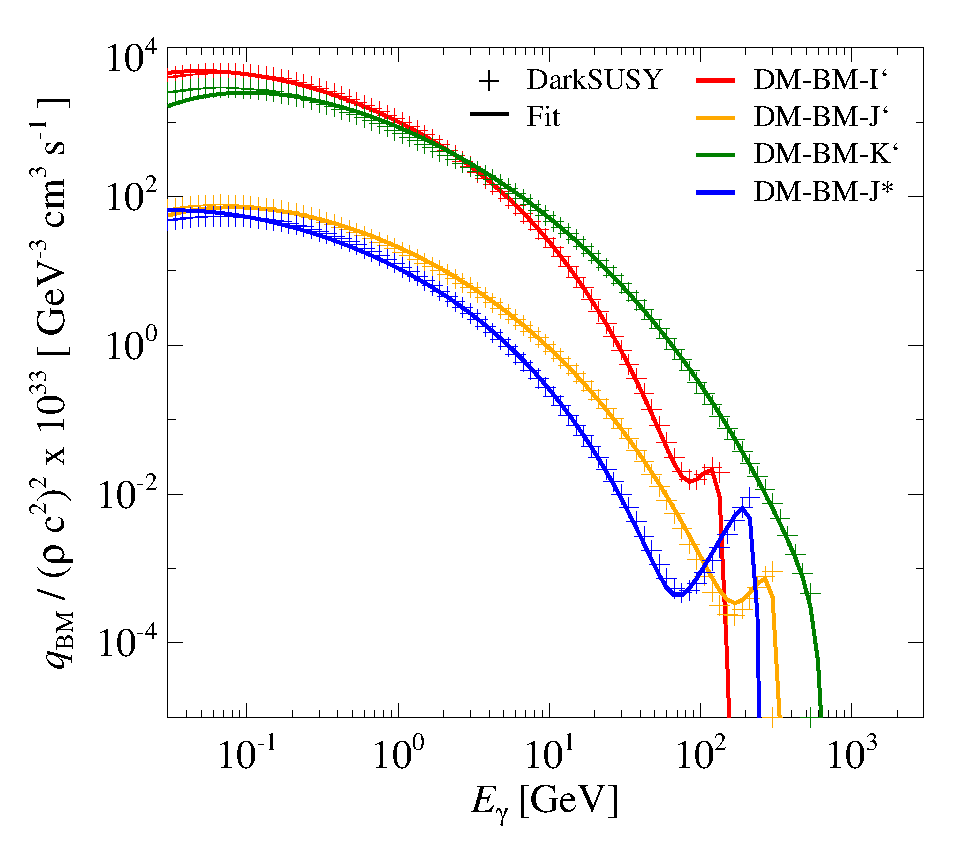
\includegraphics[width=0.49\columnwidth]{figures/fit.ds.flux.eps}
 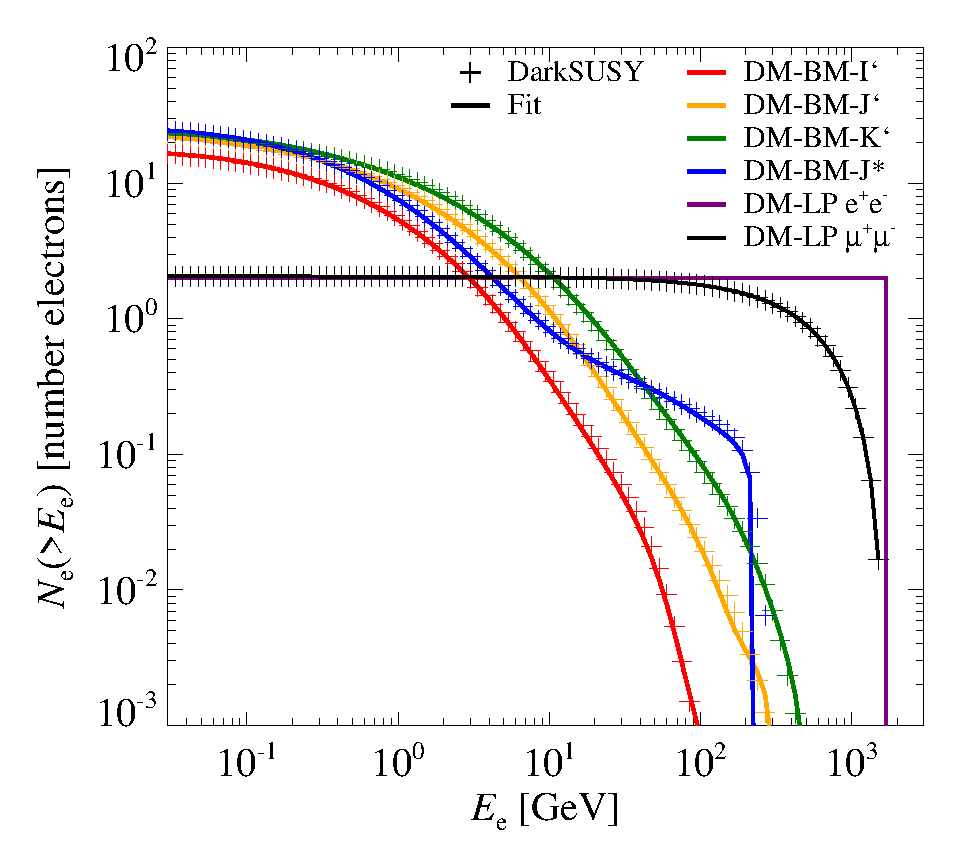
\includegraphics[width=0.49\columnwidth]{figures/fit.epflux.int.eps}
 \caption{\it Source functions for different dark matter (DM)
   models. Crosses show the simulated data from {\sc DarkSUSY}
   \cite{ds}, \C{$\times$ show the data generated by
     \protect\cite{2011JCAP...03..019C,2011JCAP...03..051C}} and the
   solid lines show the fit to the data. LEFT PANEL: normalized
   differential continuum spectra for four different DM benchmark (BM)
   models; $\Ip$ model (red), $\Jp$ (orange), $\Kp$ (green), and $\Js$
   (blue). We use Eq.~(\ref{eq:bm_cont}) to fit the continuum
   spectra. RIGHT PANEL: number of electron and positron per DM
   annihilation above the electron energy $\ee$ for different DM
   models; $\Ip$ BM model (red), $\Jp$ BM model (orange), $\Kp$ BM
   model (green), and $\Js$ BM model (blue), \C{leptophilic (LP) DM
   annihilating indirectly into electrons and positrons (purple) and
   into muons (black) without considering Sommerfeld boosts.} We use
   Eq.~(\ref{eq:bm_elec}) and Eqs.~(\ref{eq:lp_mu}-\ref{eq:lp_ep}) to
   fit the spectra of electrons and positrons from BM and LP models,
   respectively.}
 \label{fig:q_DM}
\end{minipage}
\end{figure*}


\subsection{Astrophysical modeling of DM induced emission}
\label{sect:AP}

We now turn to the detailed modeling of the surface brightness
profiles of DM annihilation emission and discuss the DM profiles for
the smooth distribution and substructures.

\subsubsection{General equations}

The differential photon flux within a given solid angle $\Delta
\Omega$ along a line-of-sight (los) is given by
\begin{equation}
\label{eq:dflux}
\frac{\dd \fg}{\dd \eg} \equiv \frac{\dd^3 \ngamma}{\dd A \,\dd t\, \dd
  \egamma} = \frac{1}{2}\int_{\Delta\Omega} \dd\psi \sin\psi \frac{\dd \sg}{\dd \eg}(\psi,\eg)\,,
\end{equation}
where
\begin{equation}
\label{eq:dtildeflux}
\frac{\dd \sg}{\dd \eg}(\psi,>\eg) = \int_{\Delta\Omega} \dd\Omega \int_{\rm los}
\dd l\, q_{\rm sum}\left(\eg,r\right)\Lambda(\theta)\,,
\end{equation}
and $\sg(\psi, >\eg)$ denotes the surface brightness above the photon
energy $\eg$.  The integration along the line-of-sight $l$, in the
direction $\psi$ that the detector is pointing, is parametrized such
that the radius of the source $r=\sqrt{l^2+D_\clu^2-2 D_\clu
  l\cos\Psi}$, where $D_\clu$ is the distance from the Earth to the
center of the cluster halo and
$\cos\Psi\equiv\cos\theta\cos\psi-\cos\varphi\sin\theta\sin\psi$. The
angular integration $\dd \Omega= \sin\theta\dd \theta \,\dd \varphi$
is performed over a cone centered around $\psi$ and the opening angle
$\Delta \Omega$ is typically taken to be a few times the point spread
function (PSF) $\psf$. The limited angular resolution results in a
probability that a photon coming from a direction $\psi$' is instead
reconstructed to a direction $\psi$, where the underlying probability
distribution follow a Gaussian:
\begin{equation}
\Lambda(\theta)=\frac{1}{2\pi\psf^2}
\,\rmn{exp}\left[-\frac{\theta^2}{2\psf^2}\right]\,,
\quad \rmn{where}\quad \theta=\psi'-\psi \,.
\end{equation}
We denote the total differential source function by $q_{\rm
  sum}(\eg,r)$, where we include contributions from five main
processes; leptophilic DM annihilating \C{through
  $\chi\,\chi\to\phi\,\phi\to\{4e,\,4\mu\to4e,\,4\pi\to4e\}$ where the
  $\rmn{e}^+/\rmn{e}^-$ pairs} IC upscatter background photons
(LP-IC), leptophilic DM emitting final state radiation (LP-FSR),
supersymmetric DM BM models where annihilating neutralinos generate
$\rmn{e}^+/\rmn{e}^-$ pairs that upscatter background photons (BM-IC)
and emit a continuum as well as final state radiation (BM-Cont), and
CR proton induced $\pi^0$ that decays into gamma-rays
(CR-$\pi^0$). The source function is given by
\begin{equation}
q_\rmn{sum} (\eg,r) = \qCR(\eg,r)+
\sum_i \,q_{\rmn{sm},i}(\eg,r)\,\B_{\rmn{tot},i}(\sigv,r)
\end{equation}
where the differential CR to gamma-ray source function is denoted
by $\qCR(\eg,r)$ (see Sect.~\ref{sect:CRs} and
\cite{2010MNRAS.409..449P} for further details). The subscript $i$
runs over the gamma-ray producing DM channels and the total
differential boost factor for DM is given by:
\begin{eqnarray}
\B_{\rmn{tot},i}(r,\sigv) = \left\{\begin{array}{cc}
\B_\sfe(\sigv)\,\B_{\sub,i}(r) &\rmn{for\,\,LP}\\
\B_{\sub,i}(r) &\rmn{for\,\,BM\,.}\end{array}\right.
\end{eqnarray}
It is the product of enhancement factors from SFE $\B_\sfe(\sigv)$
(see Eq.~\ref{eq:B_sfe} and Sect.~\ref{sect:LP}) and from substructure
enhancement over the smooth halo contribution $\B_{\sub,i}(r) =
1+\rho_{\sub,i}^2(r)/\rho^2(r)$ \C{\footnote{Note that if the boost
    from substructures is $\gg 1$, then the Sommerfeld enhancement
    approaches the constant saturated boost of 530.}} (see
Eqs.~\ref{eq:rho_sub}-\ref{eq:xvir} and Sect.~\ref{sect:subst}).  The
DM source function from the smooth halo for each process is written in
the form:
\begin{equation}
\label{eq:q_sm}
q_{\rmn{sm},i} (\egamma,r) = \sum_j
\frac{\dd \ngammaj}{\dd E_\gamma} \Gamma_j(r)\,,
\end{equation}
where the annihilation rate density is given by 
\begin{equation}
\label{eq:ann_rate}
\Gamma_j(r) = \frac{1}{2} \left[\frac{\rho(r)}{\mx}\right]^2 
\, \sigmaannv_j\,.
\end{equation}
Here, the subscript $j$ runs over all kinematically allowed gamma-ray
producing channels, each with the spectrum $\dd
  \ngammaj /\dd\eg$ and annihilation cross section $\sigmaannv_j$.
We denote the DM mass with $\mx$ and the smooth DM density profile
with $\rho(r)$.


\subsubsection{The smooth DM density profile}
\label{sect:smooth}

 Typically the universal Navarro-Frenk-White (NFW) density
profile provides a good fit to both the observed and simulated
clusters. It can be considered as a special case of the more general
5-parameter profile:
\begin{equation}
\rho(r) = \frac{\rhos}{\left(r/r_\s\right)^\beta
  \left[1+\left(r/r_\s\right)^\alpha\right]^\delta}\,,\quad
\delta=\frac{\gamma - \beta}{\alpha}\,.
\label{eq:rho_nfw}
\end{equation}
Here, $\beta$ denotes the inner slope, $\gamma$ is the outer slope,
and $\alpha$ is the shape parameter that determines the profile shape
at the scaling radius $r_\s=\rvir/c$ that characterizes the transition
between the different power-law slopes. A cuspy NFW profile is given
by $(\alpha,\beta,\gamma)=(1,1,3)$. The characteristic overdensity for
an NFW profile is given by
\begin{equation}
\rhos(c)=\frac{200\,\rhoc}{3}\,\frac{c^3}
{\log\left(1+c\right)-c/(1+c)}\,,
\label{eq:rho_s}
\end{equation}
 where the halo mass dependent concentration parameter $c$ is derived
 from a power-law fit to cosmological simulations with $\mvir \gtrsim
 10^{10} \msun$ \cite{2008MNRAS.391.1940M},
\begin{equation}
\label{eq:cfit}
  c=3.56 \times \left(\frac{\mvir}{10^{15}\,\msun}\right)^{-0.098}\,.
\end{equation}
This mass scaling agrees well with \cite{2009ApJ...707..354Z} for
cluster-mass halos after converting the concentration definitions
according to \cite{2003ApJ...584..702H}. In this work we choose to
model the DM density by an Einasto density profile
\begin{equation}
\label{eq:dens_ein}
\rho_{\rm ein}(r) = \rho_{-2}\,\exp\left\{-\frac{2}{\alpha}
  \left[\left(\frac{r}{r_{-2}}\right)^\alpha -1 \right] \right\},\,
\alpha=0.17 \,,
\end{equation}
that is slightly shallower in the center than the conventional
Navarro-Frenk-White (NFW) profile, but provides a better fit to recent
simulated high resolution DM halos
\cite{2006AJ....132.2685M,2010MNRAS.402...21N}. It should also be
noted that recent observations of the Abell 383 galaxy cluster find a
density profile with a shallower inner slope of $\beta=0.6$ compared
to an NFW profile, and $\beta\gtrsim 1$ can be ruled out with $>95$\%
confidence \cite{2011ApJ...728L..39N}. These observations are based on
lensing and X-ray measurements as well as the stellar velocity
dispersion of the central galaxy. In Eq.~(\ref{eq:dens_ein}) we denote
the density where the profile has a slope of $-2$ by $\rho_{-2}$, and
the radius by $r_{-2}=\rvir/c$. We use that the density
$\rho_{-2}(c)=\rho_\s(c)/a(c)$ and determine $a(c)$ through $\mvir$:
\begin{equation}
\int_0^{\rvir}\dd V \rho_{\rm ein} = \mvir = 
200\,\rho_{\rmn{cr}} \frac{4\pi\,\rvir^3}{3} \,.
\end{equation}
Here $a=(4.16-4.30)$ for $c=(3-10)$ and since $a$ is a slowly
increasing function with concentration $c$, we fix it for simplicity
to $a(c)\approx a \approx 4$.

In the recent dark matter simulation literature, it has become
standard to characterize halos by the value, $V_\rmn{max}$, where the
circular velocity $V_\rmn{circ}(r)=\sqrt{GM(<r)/r}$ attains its
maximum:
\begin{eqnarray}
V_\rmn{max} &=& V_\rmn{circ}(\rvir) 
\left[\frac{0.216\,c}{\log(1+c)-c/(1+c)}\right]^{0.5}\propto \mvir^{0.32}.\nonumber\\
\end{eqnarray}
Especially for subhalos, this quantity seems to be more stable
compared to the virial mass that is subject to tidal stripping. For
comparison, we quote typical values for a large galaxy cluster and a galaxy group:
\begin{eqnarray}
M_{200} = 1\times10^{15}\,\msun:\quad &&V_\rmn{max}=1480\,\rmn{km/s}, \nonumber\\
                                     &&R_\rmn{max}=0.61\,\rvir, \\
M_{200} = 4\times10^{13}\,\msun:\quad &&V_\rmn{max}=~520\,\rmn{km/s}, \nonumber\\
                                     &&R_\rmn{max}=0.44\,\rvir.
\end{eqnarray}


\subsubsection{Substructures}
\label{sect:subst}
High-resolution dissipationless DM simulations of MW type halos find substantial
amount of substructures in the periphery of DM halos, while the
substructures in the center suffer from dynamical friction and tidal
effects depleting their central number densities. Since the DM
annihilation rate depends on the density squared, the resulting flux
from substructures is boosted compared to the smooth density
distribution. Recent high resolution simulations suggest a flux
enhancement from substructures of more than 100
\cite{2008MNRAS.391.1685S, 2010ApJ...718..899A} for a MW size halo. We
adopt a boost from substructures of 230 which is the enhancement found
in one of the highest resolved MW halos ever simulated.\footnote{Note
  that these high values for boost factors are now consistently found
  in high-resolution simulations of dark matter halos \protect
  \cite{2008MNRAS.391.1685S, 2010ApJ...718..899A} after accounting for
  the tidal mass loss of subhalos. This effect causes a significantly
  flatter subhalo distribution compared to the smooth distribution and
  erroneously assuming an identical mass density distribution of smooth
  DM and substructure biases the subhalo boost factor too low
  \cite{2008JPhCS.125a2008K, 2008JPhCS.125a2008K}.} We use a double
power-law function to fit\footnote{Our approach of fitting the
  scaling behavior of $L_\sub(<r)$ directly from numerical
  simulations self-consistently accounts for the radial dependence of
  the substructure concentration \protect \cite{2008MNRAS.391.1685S}.}
the luminosity from the smooth component of substructures
(i.e. substructures within substructures are not included) inside
radius $r$ which is determined for the Aquarius simulations
\cite{2008MNRAS.391.1685S,2008Natur.456...73S}. Our best fit is given
by
\begin{eqnarray}
  L_\sub(<x) &=& a_0\,C(\mvir)\,L_{200\sm}(\mvir)\,x^{a_1
    \displaystyle{x}^{a_2}}\,,\label{eq:Lsub}\\
   a_0 &=& 0.76\,,\quad a_1 = 0.95\,,\quad  a_2 = -0.27\,, \quad 
 \nonumber\\
  C(\mvir) &=& \left(\frac{\mvir\,M_{\rm res,sim}}
{M_{\rm 200sim}\,M_{\rm lim}}\right)^{\alpha_C}
=0.023\,\left(\frac{\mvir}{M_{\rm lim}}\right)^{\alpha_C}.\nonumber\\
\label{eq:Csub}
\end{eqnarray}
Here, $\alpha_C=0.226$, $a_i$ denote our fit variables, $L_{200\sm}$
is the luminosity from the smooth halo without substructures within
$\rvir$ and $x= r/\rvir$.  We derive the normalization function
$C(\mvir)$ in Eq.~(\ref{eq:Csub}) from the simulations in reference
\cite{2008Natur.456...73S} using a value of $M_{\rm
  200sim}=1.9\times10^{12}\msun$ for the mass of the MW halo in the
simulation and $M_{\rm res,sim}=10^5\msun$ for the mass of the
smallest resolved subhalos in the MW simulation.  The smallest mass of
subhalos in reality, $M_{\rm lim}$, is determined from the free
streaming length of DM at decoupling---an effect that erases structure
on scales smaller than the free streaming length. In applying
Eq.~(\ref{eq:Csub}), we implicitly assume that the mass power-law
scaling relation is valid down to the free streaming mass of DM
halos. In the CDM universe, this is conventionally taken to be
$10^{-6}\msun$ \cite{2001PhRvD..64h3507H, 2005JCAP...08..003G} (see
\cite{2009NJPh...11j5027B} for a discussion of the range expected in
various DM models). Note that potentially the power-law could flatten
towards smaller mass scales although current simulations show no hints
of such a behavior and since Einstein's gravity is a scale-free
theory, we do not expect such a behavior on theoretical grounds
either.  For DM halos more (less) massive than the MW we expect a
larger (smaller) boost from substructures, simply because of the
larger (smaller) mass range down to the minimum mass $M_\rmn{lim}$.

\C{To motivate the scaling of the substructure luminosity boost with
  limiting substructure mass in Eqs.~(\ref{eq:Lsub}-\ref{eq:Csub}),
  we show how it derives from the substructure mass function, $\dd
  N_\sub/\dd M \propto M^{-1.9}$
  \cite{2008MNRAS.391.1685S,2008Natur.456...73S} and substructure
  luminosity scaling, $L_\sub \propto M^A$. The total luminosity of
  substructures scales as
\begin{eqnarray}
  L_\rmn{sub,tot} &=& L_\sub\,N_\sub = L_\sub 
\int \dd M \frac{\dd N_\sub}{\dd M} \nonumber\\
 &\propto& M^{A-0.9} \propto M^{-0.226}\,,\quad
\rmn{for}\quad A=0.674\,. \nonumber\\
&&
\end{eqnarray}
Tidal truncation is responsible in shaping the substructure luminosity
scaling parameter $A$. Here we only sketch out qualitative arguments
and leave the details to future work. First, tidal effects truncate
the subhalo profile primarily in the outer regions. As a result of
this, the subhalo acquires a steeper logarithmic slope than the
canonical 3 from the NFW-profile. Second, tidal stripping imposes a
mass-dependency and should be stronger for smaller substructure. While
the stripping efficiency (for an effective cross section $\sigma$)
only depends on the density since the mean free path scales as
$x_\rmn{mfp} \propto 1/(n_\rmn{dm} \sigma)$, there is less mass at any
given density for smaller substructures. Hence, modest density
inhomogeneities in the host halo seen by the orbiting substructures
cause a stronger mass loss of these smaller satellites. Third, the
tidal truncation radius should be a function of host halo radius due
to the increasing smooth density profile for smaller radii.  If we
pick an effective host halo radius which dominates the luminosity
contribution of the substructures and were to fit the tidally
truncated subhalo density profile with an NFW-profile, the resulting
$\rs$ would be biased toward lower values implying a higher
concentration compared to an isolated halo. In order to reproduce our
value of $A$, we would need a concentration mass relation of $c\propto
M^{-0.14}$.  As expected, this is steeper than the concentration-mass
relation found for isolated halos on dwarf galaxy scales, $c \propto
M^{-0.06}$ \cite{2011arXiv1101.2020I}, as well as galaxy and cluster
scales, $c \propto M^{-0.098}$ \cite{2008MNRAS.391.1940M}.}

We now derive the squared density profile for the substructures
using
\begin{eqnarray}
\rho_\rmn{sub}^2(r) &=& \frac{\dd L_\rmn{sub}}{\dd V} \frac{1}{A_{\rmn{dm}}}\,,\label{eq:rho_sub}\\
L_{200\sm} &=&  A_{\rmn{dm}} \int_{\rvir} \dd r' 4\pi r'^2 \rho^2(r')\,,\label{eq:Lsm}\\
 \frac{\dd L_\rmn{sub}}{\dd V} &=& a_0\,a_1\,C(\mvir)\,x^{a_2+a_1\,x^{a_2}}\,
\left[\frac{1+a_2\log(x)}{4\pi\,r^3}\right]\,,\nonumber\\
\\
x &=& r/\rvir\,.\label{eq:xvir}
\end{eqnarray} 

The different density profiles have some impact on the luminosity from
annihilating DM, although the details of the density profile can be
neglected compared to the dominating boost from substructures
(assuming DM to be cold). In Fig.~\ref{fig:radial_lum} we compare the
radial dependence of the accumulative luminosity from different smooth
cluster density profiles to the boosted luminosity due to substructure
for different mass scales. We recalculate the overdensity, $\rhos$,
for the shallower density profile with $\beta=0.6$ and rescale the
concentration parameter in Eq.~(\ref{eq:cfit}) with $300/160$
\cite{2011ApJ...728L..39N} to account for the more centralized scale
radius in cluster with a shallow inner slope. The emission of this
profile with $\beta=0.6$ is about 30\% larger within $\rvir$ compared
to a cuspy NFW ($\beta=1.0$).  This difference is built up within
$0.1\rvir$ (i.e. close to $r_\s$). Hence the slope of the central part
of a cluster has little influence for the DM luminosity within $\rvir$
as long as the degeneracy in the lensing mass measurements with $r_\s$
(which decreases for decreasing inner slope) has been taken into
account. The emission from an Einasto density profile is about 50\%
larger than the cuspy NFW profile in the periphery of the cluster,
where the difference is mainly built up at a few percent of
$\rvir$. The increase in luminosity due to substructures is neglible
in the center of halos, but integrated out to $\rvir$ the boost
relative to the smooth emission profile amounts to approximately 20
for dwarf galaxies, $200$ for galaxies, and $10^3$ for galaxy
clusters. These boost factors are only realized for direct
annihilation emission (continuum emission or final state radiation) or
IC scattering off homogeneous seed photon fields (CMB). For IC
scattering of SD photons, the overlap of final state leptons and SD
photons is smaller which causes the substructure boost over the smooth
emission to be reduced by roughly two orders of magnitudes. \C{It
  should also be noted that the substructure boosted fluxes from
  clusters are much more extended than for dwarf galaxies, hence more
  difficult to detect with Cherenkov telescopes. In fact, it was shown
  in Sanchez-Conde et al. \cite{2011arXiv1104.3530S} that inside
  $0.1$~deg, where the sensitivity of Cherenkov telescopes is
  maximized, the expected DM flux including substructures from the
  brightest dwarf galaxy is about an order magnitude higher than the
  brightest cluster. However, that work assumed a substructure boost
  of about 50 in the most massive cluster halos which is more than an
  order magnitude smaller than what we use in this work, hence in
  projection we expect this difference to be a factor few smaller.}

\begin{figure}%[t]
 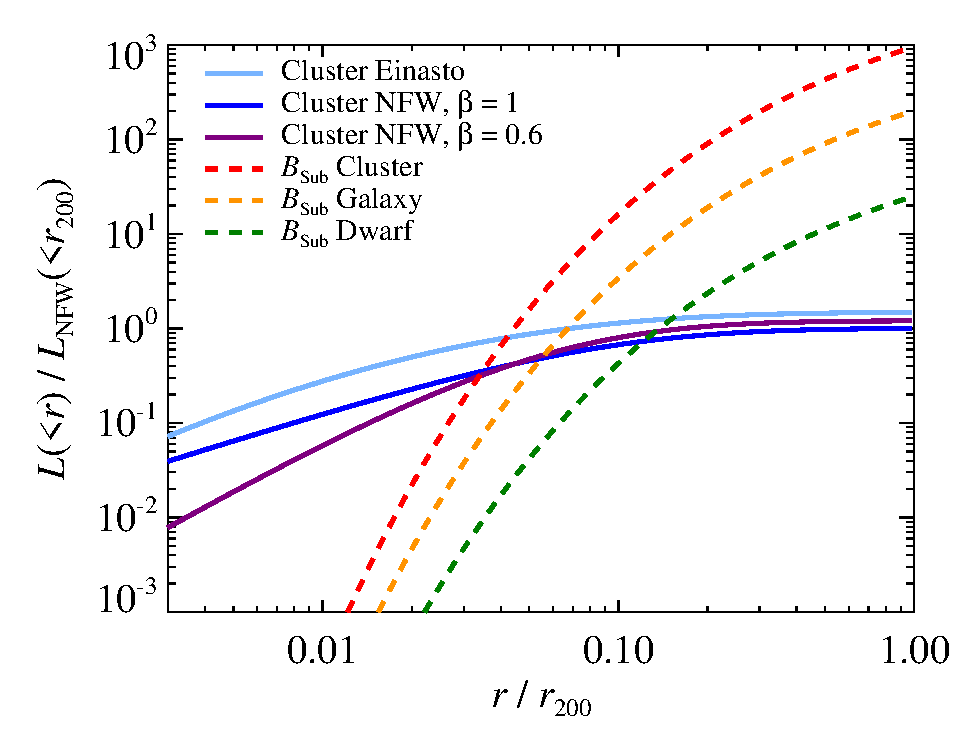
\includegraphics[width=0.99\columnwidth]{figures/dens.prof.eps}
 \caption{\it Radial dependence of DM annihilation luminosity of
   smooth halo and substructures. The solid lines show the
   accumulative smooth luminosity from a cluster with the mass
   $\mvir=10^{15}\,\msun$ for three different density profiles; an
   Einasto profile with $\alpha=0.17$ (light blue), a cuspy NFW
   profile with $\beta=1.0$ (dark blue), and a core NFW profile with
   $\beta=0.6$ (purple). The dashed lines show the accumulative
   luminosity from substructures for three different mass scales; an
   $\mvir=10^{15}\,\msun$ galaxy cluster (red), an
   $\mvir=10^{12}\,\msun$ galaxy (orange), and an
   $\mvir=10^{8}\,\msun$ dwarf galaxy (green). All luminosities have
   been normalized with the luminosity within $\rvir$ from a cuspy NFW
   profile. We have assumed the standard value for the limiting
   substructure mass of $M_\rmn{lim}=10^{-6}\,\msun$. Note the large
   expected boost from substructures in clusters ($\sim1000$), and the
   relative small boost in dwarf galaxies ($\sim20$).}
 \label{fig:radial_lum}
\end{figure}

In Fig.~\ref{fig:radial_emis} we show the radial regions that dominate
the DM annihilation luminosity, in particular we show the differential
contribution to the DM luminosity per logarithmic interval in radius
for three different mass scales. Solving for the maximum of this
curve, $\dd^2L_{200\sm}/\dd (\log x)^2=0$ in combination with
Eq.~(\ref{eq:Lsm}), we find that the luminosity from the smooth NFW
profile peaks at $r \simeq \rvir/3c$. Despite the cuspy nature of the
density profile, the luminosity is not dominated by the central region
but by the transition region where the profile steepens because of the
larger volume available there. For large clusters with typical
concentrations of $c = \rvir/r_\s \simeq 4$, the luminosity from the
smooth profile is focused to the regime around 10\% of $\rvir$.  In
contrast, emission from substructures is mainly contributed by the
outer parts of DM halos. As shown in Fig.~\ref{fig:radial_emis}, the
product of annihilation emissivity and emission volume increases
towards $\rvir$ and only starts to drop outside this radius.  Note
that, even though most of the substructure mass density has been
erased in the central regions of DM halos, a cluster in projection has
a significant enhancement due to substructures at a radius of just a
few percent of $\rvir$. 
\begin{figure}
  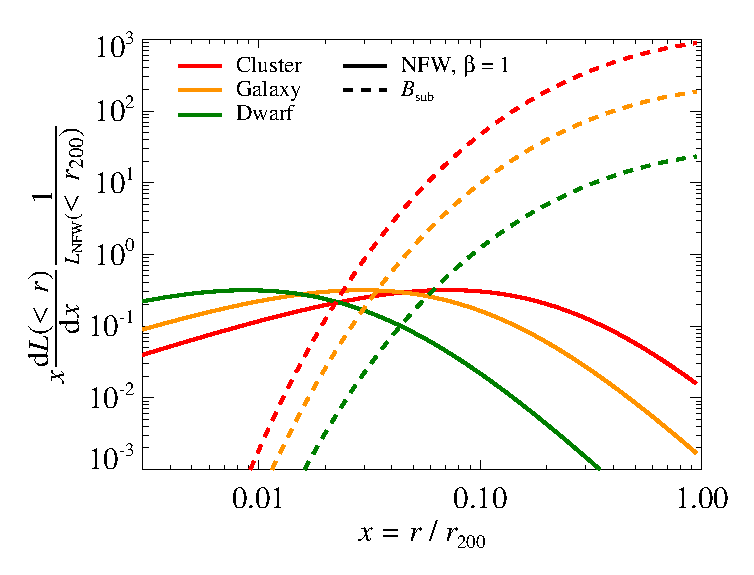
\includegraphics[width=0.99\columnwidth]{figures/emissiv.sub.eps}
  \caption{\it Plot that shows where most of the DM annihilation
    luminosity originates.  We show the differential contribution to
    the DM annihilation luminosity per logarithmic interval in radius
    which corresponds to $x^3\rho^2/\rho^2_{200}$ where $\rho_{200}$
    is the density at $\rvir$. The solid lines represent cuspy
    $\beta=1.0$ NFW density profiles for three different mass scales;
    an $\mvir=10^{15}\,\msun$ galaxy cluster (red), an
    $\mvir=10^{12}\,\msun$ galaxy (orange), and an
    $\mvir=10^{8}\,\msun$ dwarf galaxy (green). The dashed lines show
    the contribution from substructures for the same three mass
    scales. All luminosities have been normalized with the luminosity
    within $\rvir$ from a cuspy NFW profile. We have assumed the
    standard value for the limiting substructure mass of
    $M_\rmn{lim}=10^{-6}\,\msun$. For the smooth profile, the majority
    of the flux is delivered by a region around $r_\s/3$ as indicated
    by the maximum value of the curves. In contrast, for substructures
    the emission is dominated by regions around $r_{200}$.}
  \label{fig:radial_emis}
\end{figure}


\subsection{Inverse Compton emission}
\label{sect:IC}

In this section we outline the basics of inverse Compton (IC)
emission. As target radiation fields we consider  cosmic microwave
background (CMB) photons, and the light from stars and dust (SD). We
derive an analytic model from which we can estimate the spectral
and spatial distributions of SD as a simple function of cluster mass.

The standard IC source function is given by
\cite{1979rpa..book.....R}:
\begin{eqnarray}
  q_{\rmn IC}(\eg, r) &=&  \frac{\dd^3 N_\gamma}{\dd V\,\dd t\,\dd \eg} = 
 \frac{3}{4}c\,\sigma_\rmn{T}
\int\dd \eph \frac{n_\rmn{ph}(\eph)}{\eph}\nonumber\\
&\times& \int \dd \ee\,\frac{\dd n_\e}{\dd \ee}(\ee,r)\,
 \frac{\left(m_\e c^2\right)^2}{\ee^2}G(\Gamma_\e,q)\,,\nonumber\\
  \label{eq:ICemiss}
\end{eqnarray}
where $\ee$ is the energy of the upscattering electrons and $\eph$ is
the energy of the background photon field. We represent the Thomson
cross section with $\sigma_\rmn{T}$ and the full differential
Klein-Nishina (KN) cross section is captured by
\cite{1970RvMP...42..237B}:
\begin{equation}
\label{eq:KN_spec}
G(\Gamma_\e,q) = 2q\ln{q}+(1+2q)(1-q)+ 
\frac{1}{2}\frac{\left(\Gamma_\e q\right)^2\left(1-q\right)}
     {1+\Gamma_\e q}\,,
\end{equation}
where
\begin{equation}
\Gamma_\e=\frac{4\eph \ee}{\left(m_\e c^2\right)^2}\,,\qquad \rmn{and} \qquad  
q=\frac{\eg}{\Gamma_\e\left(\ee-\eg\right)}\,.
\end{equation}
The full KN cross section accounts for the less efficient energy
transfer between the photon and electron once the energy of the
Lorentz-boosted photon in the electron rest frame comes close to $m_\e
c^2$ such that the scattering electron experiences a significant
recoil. This results in a steepening of the IC gamma-ray spectrum. In
the low energy Thomson regime the IC spectrum $F_\gamma\sim
E_\gamma^{-(\alpha_\e-1)/2}$, however when $\Gamma_\e \gg 1$ the IC
spectrum steepens due to the KN suppression to
$\eg^{-\alpha_\e}\log(\eg)$. Here we denote the steady state electron
spectrum by $\alpha_\e$.

We account for two major contributions to the number density of
radiative background fields $n_\ph$; the CMB photons and the infra-red
(IR) to ultra-violet (UV) light emitted by SD. The number density for
the SD is given by $n_\ph\equiv\dd^2 N_\ph/ (\dd V \,\dd \eph)
(\eph,r)= u_\sd(\eph,r) /\eph^2$ where the specific SD energy
density $u_\sd(\eph,r)$ is given in the Appendix,
Eq.~(\ref{eq:u_SD_er}). We model the CMB photon spectrum as a photon
gas that is isotropically distributed and follows a black body
spectrum with the temperature $T=2.73\,$~K:
\begin{equation}
\label{eq:photon_gas}
  n_\rmn{ph}(\eph) = \frac{\dd^2 N_\ph}{\dd V \,\dd \eph} =
  \frac{1}{\pi^2(\hbar c)^3}\frac{\eph^2}{\exp(\eph/k_\B T)-1}\,.
\end{equation}
Note that the typical energy of a black body photon before scattering
is given by $\langle\eph\rangle=\epsilon_\ph/\tilde{n}_\ph\approx\,2.7\, k_\B T$,
where $\tilde{n}_\ph$ and $\epsilon_\ph$ are the number- and
energy-density derived by integrating $n_\ph(\eph)$ and $\eph
n_\ph(\eph)$ over the photon energy $\eph$, respectively.

The electrons injected from annihilating DM also suffer from diffusive
and radiative losses. Hence we have to calculate the equilibrium
spectrum of the electrons plus positrons denoted by $\dd n_\e/\dd \ee$
in Eq.~(\ref{eq:ICemiss}). We derive this stationary solution using
the cosmic ray transport equation (neglecting convection and
re-acceleration effects):
\begin{eqnarray}
\label{eq:CRdiffusion}
\frac{\partial}{\partial t}\left(\frac{\dd n_\e}{\dd \ee}\right) = 
&\nabla& \left[D\left(\ee,\bx\right)\nabla\frac{\dd n_\e}{\dd \ee}\right] + 
\frac{\partial}{\partial \ee}
\left[b\left(\ee,\bx\right) \frac{\dd n_\e}{\dd \ee}\right]
 \nonumber \\
&+& q_\e(\ee,\bx)\,,
\end{eqnarray}
where $D(\ee,\bx)$ denotes the diffusion coefficient and $b(\ee,\bx)$
the energy loss term. The source function $q_\e(\ee,\bx)$ yields the
number of electrons and positrons produced per unit time, energy and
volume element at the position $\bx$:
\begin{equation}
q_\e(\ee,r)=\sum_f\frac{\dd N_\e^f}{\dd \ee}(\ee) B_f \Gamma_f(r) \,,
\end{equation}
where the annihilation rate density $\Gamma_f(r)$ is defined in
Eq.~(\ref{eq:ann_rate}). The sum runs over the kinematically allowed
annihilation final states $f$, each with a branching ratio $B_f$ and a
differential spectrum $\dd N_\e^f/\dd \ee$ that represents the number
of electrons plus positrons resulting from an annihilation
event. \del{For neutralinos annihilating directly into electrons and
  positrons we model the spectral distribution with $\dd N_\e^f/\dd
  \ee= 2\delta(\ee-m_\chi c^2)$.} \C{We use the differential spectra
  derived from high-statistics simulations in
  \cite{2011JCAP...03..019C,2011JCAP...03..051C} to compute the
  cumulative number of electrons and positrons resulting from
  neutralinos annihilate indirectly into $e^+/e^-$ pairs as well as
  $\mu^+/\mu^-$ pairs in the LP model. We use \ds to compute the
  $e^+/e^-$ spectra from our four BM models where only a fraction of
  the annihilating neutralinos is converted into electrons and
  positrons (see Sect.~\ref{sect:PF} and Fig.~\ref{fig:q_DM} for
  further details).}
%(see \cite{2009JCAP...01..016B} and references therein,
%also see fit).  

The electrons and positrons loose their energy on a timescale that is
shorter than the diffusive timescale in the ICM of galaxy clusters for
cosmic ray electrons which is larger than the Hubble time in our
energy range \cite{1997ApJ...487..529B,2011A&A...527A..99E}. Hence, we
neglect the first term of the r.h.s. in Eq.~(\ref{eq:CRdiffusion}),
and derive an expression for the equilibrium number density:
\begin{eqnarray}
{\frac{\dd n_\e}{\dd \ee}}\left(\ee, r \right) &=&
 \frac{1}{b(\ee, r)} \int_{\ee}^{\mx c^2} \dd \ee' \, 
  q_\e(\ee', r),
\label{eq:nds}\\
b(\ee,r) &=& \tilde{b}
\left[\frac{B^2_{\rm CMB}}{8\pi}+\frac{B^2(r)}{8\pi}+u_\sd(r)\right] \ee^2\,,
\\\tilde{b}&=&\frac{4\sigma_{\rm T}c}{3(m_{\rm e}c^2)^2}\,.
\end{eqnarray}
Here we include the three main radiative loss processes for the cosmic
ray electrons and positrons: (1) IC losses on CMB photons with the
equivalent field strength of the CMB of $B_{\rm
  CMB}=3.24\mu\rmn{G}\,(1+z)^2$, where $z$ is the cosmological
redshift. (2) Synchrotron losses on ambient magnetic fields where we
parameterize the magnetic field in the galaxy cluster by $B(r) =
3\mu\rmn{G} \,[n_{\rm e}(r)/n_{\rm e}(0)]^{\alpha_\B}$. We adopt a
magnetic decline of $\alpha_\B=0.7$ in this work which follows from
flux frozen magnetic fields. (3) IC losses on starlight and dust with
an energy density $u_\sd(r)$ given by Eq.~(\ref{eq:u_SD_r}), where
  we outline the derivation in the following.

The emission of galaxy clusters at infra-red (IR) and ultra-violet
(UV) wavelengths emerges from dust and starlight in both the galaxies
and the ICM (e.g. \cite{2006ApJ...648L..29P} and
\cite{2009MNRAS.399.1694G}). Three distinctive components dominate
these wavelengths: a central galaxy, the intra-cluster light (ICL),
and individual cluster galaxies. We decided to use the accurately
measured spectral shape of dust and starlight in the interstellar
medium of our Galaxy to model the emission from clusters. We then
normalize the two spectral components -- far IR dust and starlight at
wavelengths ranging from the near IR to UV -- individually by using
stacked cluster data and employ a measured mass-to-starlight
luminosity scaling relation derived from observations of the brightest
cluster galaxy (BCG) \cite{2010ApJ...713.1037H}.

In Fig.~\ref{fig:SD_spectra} we characterize the spectral shape
through a fit to the galactic spectra presented in
\cite{2006ApJ...648L..29P}.  The figure is showing the spectra at
$r=0.03\rvir$, which is the radius there the SD energy density of a
galaxy cluster equals the energy density of the CMB black-body
distribution. Inside this central radius the SD component is
dominating, which is shown in Fig.~\ref{fig:SD_Edens} where we compare
the energy densities from different radiation fields in a galaxy
cluster with the mass $\mvir=6.0\times10^{14}\msun$. For this figure we
use two different profiles for the SD energy density, where the total
profile includes the contribution from the ICL, the BCG and all the
galaxies, while the galaxies are excluded in the smooth profile. To
compute the IC emission from SD, we require a non-negligible overlap
of the relativistic lepton distribution resulting from DM annihilation
and SD.  In fact, one can show with a simple order of magnitude
calculation that the overlap, $f_\rmn{IC-ol}$, of the photon field of
individual galaxies (starlight and dust emission) and the smooth DM
density is very small so that we can neglect the starlight
contribution from galaxies to the IC emission for the reminder of this
work,
\begin{eqnarray}
\label{eq:SD_overlap}
f_\rmn{IC-ol} = \frac{N_\rmn{gal} V_\rmn{gal} f_\rmn{light}}{V_\rmn{clu}}
\lesssim  \frac{N_\rmn{gal} M_\rmn{gal}}{M_\rmn{clu}\,c_\rmn{gal}^{3}}=10^{-4}.
\end{eqnarray}
Here we assume that the exponential scale height of the stellar light
is less than the scale radius of the galaxy halo, $f_\rmn{light}
\lesssim (r_\rmn{s} / r_{200,~\rmn{gal}})^3 \sim c_\rmn{gal}^{-3} \sim
10^{-3}$ and $N_\rmn{gal} M_\rmn{gal} \sim 0.1 M_\rmn{clu}$. We denote
the number of galaxies within $\rvir$ with $N_\rmn{gal}$ and the
concentration of a galaxy DM halo with $c_\rmn{gal}$.

We find that even for a cluster with a relative small mass the energy
density of the SD components dominates over the CMB and the magnetic
fields (with a central B field of 3~$\mu G$) within about 10\% of
$\rvir$. Outside this radius the CMB is dominating the energy density
of the cluster.  Note that while the magnetic field is always
subdominant in the cluster for our assumptions, we keep its
contribution to the total energy density for consistency. Also note
that we extract the spatial distribution of the SD light in clusters
from a stacked emission analysis of Sloan Digital Sky Survey (SDSS)
data at the redshift $\sim 0.25$ \cite{2005MNRAS.358..949Z} and do not
attempt to correct for a potential evolution in this component
(c.f. Fig.~\ref{fig:SD_spatial}).

The spatial distribution of light emitted by SD is quite different
from what is expected for the IC upscattered SD photons. We illustrate
this in Fig.~\ref{fig:SD_lum}, where the accumulative luminosity from
SD is compared to the IC SD photons for a
$\mvir=6.0\times10^{14}\,\msun$ cluster where the boost from
substructures is excluded. The gamma-ray luminosity from IC
upscattered SD photons is dominated from the inner parts where there
is the largest overlap of the cuspy DM profile and the peaked SD
distribution. This is in marked contrast to the accumulative SD
luminosity in the optical that is dominated by the outer parts of the
cluster. Interestingly, it rises as a function of radius and follows
the distribution of an NFW mass profile outside $0.1\rvir$.  In the
center, the electrons and positrons mainly cool by IC upscattering SD
photons, hence the spatial dependence of the cooling cancels the
distribution of the SD source function, which results in a
distribution that approaches a density square profile in the center.
We also find that the luminosity within $\rvir$ from the total SD
model is a factor three larger compared to the more realistic smooth
SD model.

\begin{figure}%[t]
 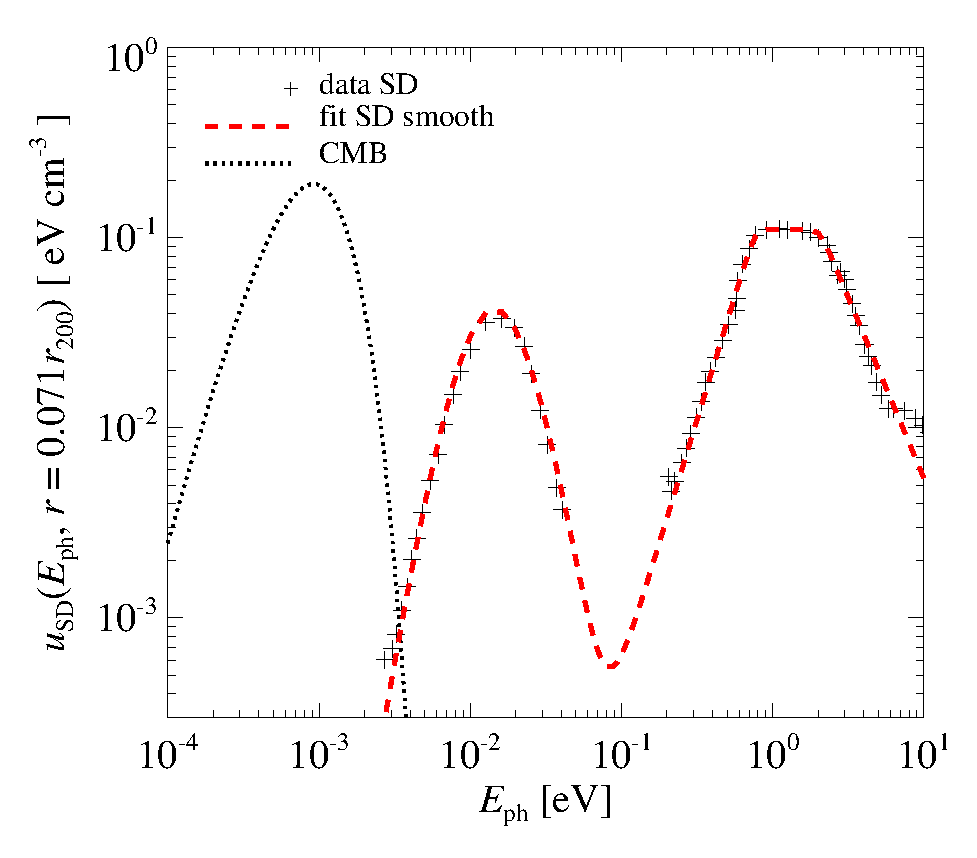
\includegraphics[width=0.99\columnwidth]{figures/fit.porter.v2.eps}
 \caption{\it Spectral dependence of radiation fields in a cluster of
   galaxies. The black dotted line of the left peak show the spectrum
   of CMB photons using a black body with a temperature of
   $2.73$~K. The crosses of the middle and right peaks represent the
   measured spectra from stars extending from the near IR to UV and
   dust at far IR wavelengths (SD), respectively, and are derived in
   \protect \cite{2006ApJ...648L..29P} for a galaxy. We normalize the
   individual SD spectrum separately using the observed luminosity
   from SD in clusters. The SD luminosity is related to the cluster
   mass through Eqs.~(\ref{eq:E_SD}-\ref{eq:N_dust}), where we use
   have used the mass $\mvir=6.0\times10^{14}\msun$ in this figure. We
   renormalize the SD spectra to the radius $r=0.03\rvir$, where the
   smooth energy density of the SD light (see Fig.~\ref{fig:SD_Edens})
   equals the energy density of the CMB. The red dashed lines show the
   fitted SD spectral model.}
 \label{fig:SD_spectra}
\end{figure}
\begin{figure}%[t]
 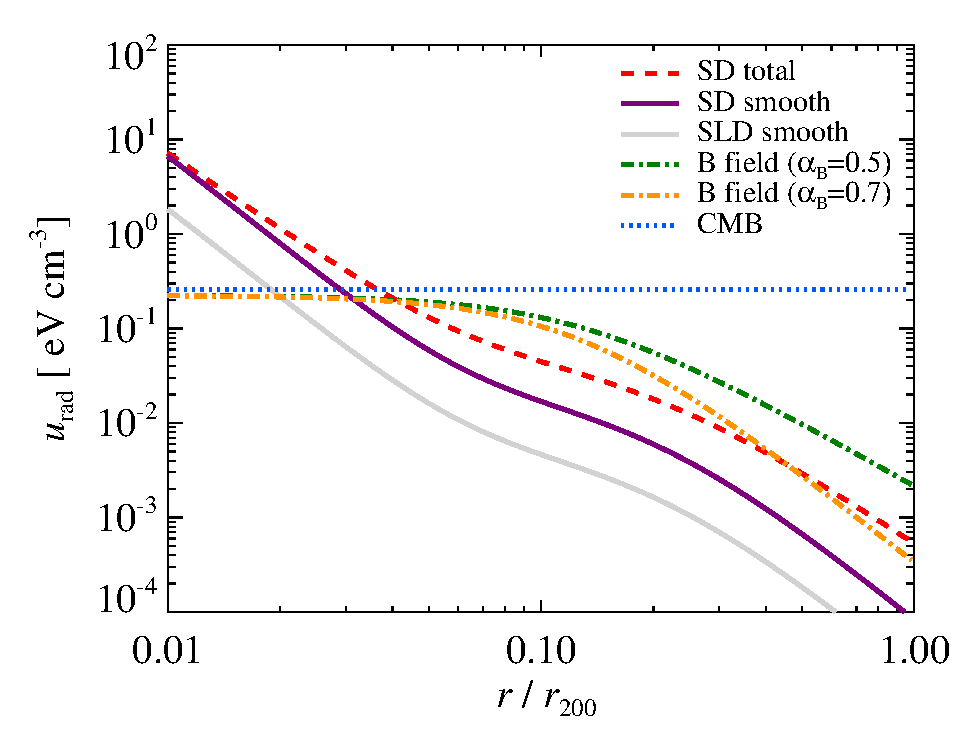
\includegraphics[width=0.99\columnwidth]{figures/ucool.eps}
 \caption{\it Spatial dependence of the energy density of radiation
   fields in a cluster of galaxies. The energy density of the CMB
   (blue dotted line) is isotropic with
   $u_\rmn{cmb}=0.26\,\rmn{eV}\,\rmn{cm}^{-3}$. The energy density of
   the light from stars and dust (SD) is denoted by the red dashed
   line and the solid purple line for the total SD light and the
   smooth SD light, respectively. For comparison we show the energy
   density of the stars and a low dust model (SLD) with the light grey
   line. The SD light has been renormalized to a cluster with the mass
   $\mvir=6.0\times10^{14}\msun$. Finally we show the energy density of two
   magnetic field models with a central magnetic field of 3~$\mu
   G$. The magnetic field scales with the gas density to the power
   $\alpha_\rmn{B}$; green dash-dotted line ($\alpha_\rmn{B}=0.5$) and
   orange dash-dotted line ($\alpha_\rmn{B}=0.7$). Note that the SD
   radiation is dominating the energy density inside
   $\sim0.03\,\rvir$.}
 \label{fig:SD_Edens}
\end{figure}

\begin{figure}%[t]
 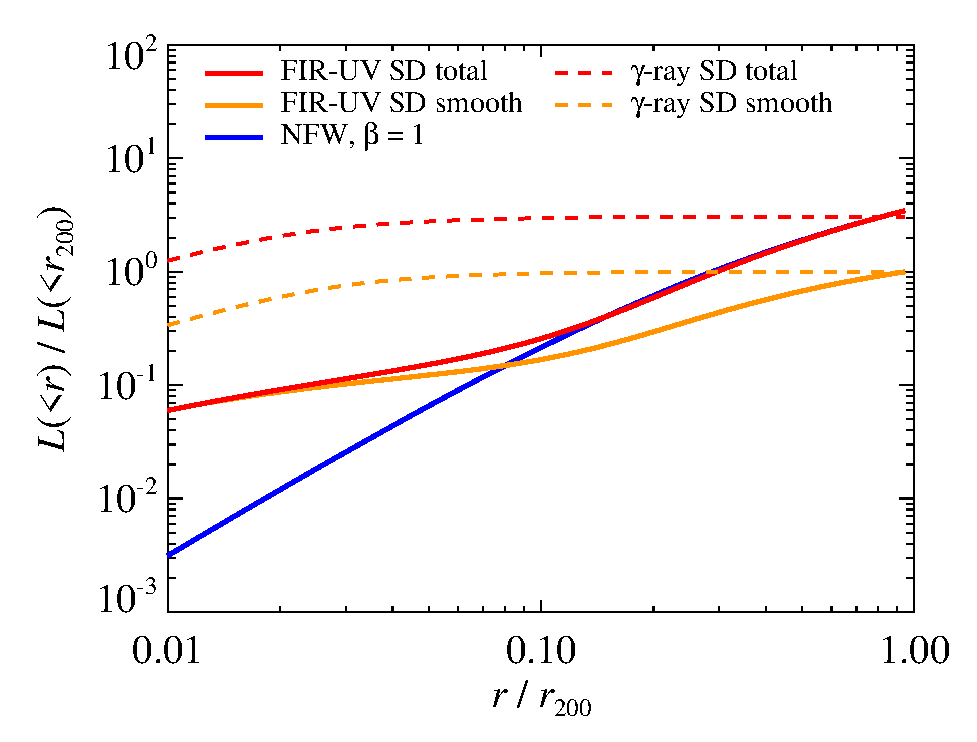
\includegraphics[width=0.99\columnwidth]{figures/lum.stars.eps}
 \caption{\it Accumulative luminosity as a function of radius. We show
   the luminosity without substructures inside radius $r$. The solid
   lines show the optical/IR emission from stars and dust (SD) and the
   IC upscattered SD light is shown by the dashed lines. The red lines
   show the total emission including the brightest cluster galaxy, the
   intra-cluster light and the additional intra-cluster galaxies,
   while these galaxies have been cut out in the smooth component
   shown by the orange lines. We normalize the SD light and the IC
   upscattered SD with the smooth luminosity within $\rvir$ for each
   component. We find that the gamma-ray IC luminosities are dominated
   by the central regime, while the SD light is mainly build up in the
   outer parts of the cluster. For comparison, we show that the SD
   light traces the NFW mass profile (blue) outside $0.1\rvir$.}
 \label{fig:SD_lum}
\end{figure}


\subsection{Cosmic-ray induced gamma-ray emission}
\label{sect:CRs}

In supernovae remnants and on scales of galaxies, there are convincing
evidences of non-thermal populations. Especially, in the MW, the
cosmic rays are observed directly as well as indirectly through radio,
X-ray, and gamma-ray emission. On larger scales of the order of few
100~kpc up to Mpc, there are currently a vast number of observations
of radio emission coming from radio mini halos in the center of
cooling flow clusters, radio relics in the periphery of clusters
\cite{2004rcfg.proc..335K} as well as smooth giant radio halos that
have been observed in more than 50 clusters
\cite{2003ASPC..301..143F,2008SSRv..134...93F}. This type of emission
is expected in clusters since the formation process of a galaxy
cluster is a very energetic processes that induces both turbulence as
well as frequently occurring merging and accretion shocks which both
are thought to accelerate relativistic non-thermal protons and radio
emitting electrons to high energies. Thus most of the observed radio
emission in clusters is expected to emerge from cosmic-ray electron
induced radio synchrotron emission. The precise origin of these
electrons, in especially relics and giant radio halos, is still not
settled. One possible scenario for the production of these electrons
are hadronic CR interactions with ambient gas protons which results in
the production of both charged and neutral pions that decay into
electrons, neutrinos, and gamma-rays (see
\cite{1980ApJ...239L..93D,1982AJ.....87.1266V,1999APh....12..169B,2000A&A...362..151D,2001ApJ...559...59M,2003MNRAS.342.1009M,2004A&A...413...17P,2004MNRAS.352...76P,2008MNRAS.385.1211P,2008MNRAS.385.1242P,2009JCAP...09..024K,2010MNRAS.401...47D,2010MNRAS.407.1565D,2010ApJ...722..737K,2011A&A...527A..99E}
).\footnote{An alternative scenario is the second order turbulent
  re-acceleration through the interaction of a previously injected
  relativistic population of electrons by supernova driven winds or
  active galactic nuclei with plasma waves and
  magneto-turbulence. \protect
  \cite{1987A&A...182...21S,1993ApJ...406..399G,2004MNRAS.350.1174B,2005MNRAS.363.1173B,2007MNRAS.378..245B,2011MNRAS.410..127B,2009A&A...507..661B}}
Supporting evidence comes from the smoothness of the extended radio
emission that often resembles that observed in thermal X-rays. This
can be easily achieve in the hadronic model since the long cooling
time of cosmic ray protons (CRs) allows for an extended and large
population of CRs to build up over the cluster history
\citep{1996SSRv...75..279V, 1997ApJ...477..560E,
  1997ApJ...487..529B}. The production of these secondaries depend
both on the gas and CR densities in the cluster, where the CR
density roughly traces the gas outside the core regime and is slightly
enhanced in the center.  This density scaling implies that clusters
are great targets for Cherenkov telescopes with a high sensitivity for
the central parts of nearby clusters. Detecting the cluster gamma-ray
emission is crucial in this respect as it potentially provides the
unique and unambiguous evidence of CR populations in clusters through
observing the $\pi^0$ bump at about 100~MeV in the spectra. 

We adopt the universal spectral and spatial gamma-ray model developed
by Pinzke \& Pfrommer \cite{2010MNRAS.409..449P} to estimate the
emission from decaying $\pi^0$:s that dominates over the IC emission
from primary and secondary electrons above 100~MeV in clusters. The
gamma-ray formalism was derived from high resolution simulations of
clusters of galaxies that included radiative hydrodynamics, star
formation, supernova feedback, and followed CR physics using a novel
formulation that trace the most important injection and loss processes
self-consistently while accounting for the CR pressure in the
equation of motion
\cite{2008A&A...481...33J,2007A&A...473...41E,2006MNRAS.367..113P}.
We note that the overall normalization of the CR and gamma-ray
distribution scales with the maximum acceleration efficiency at
structure formation shock waves. Following recent observations at
supernova remnants \cite{2009Sci...325..719H} as well as theoretical
studies \cite{2005ApJ...620...44K}, we adopt a realistic value of this
parameter and assume that 50\% of the dissipated energy at strong
shocks is injected into CRs while this efficiency rapidly decreases
for weaker shocks \cite{2007A&A...473...41E}. As a caveat we note that
the analytic model is based on simulations that only considered
advective transport of CRs by turbulent gas motions which produces
centrally enhanced profiles. However active CR transport such as CR
diffusion and streaming tends to drive the CR radial profiles towards
being flat, with equal CR number density everywhere. While the CR
streaming is then usually larger than typical advection velocities and
becomes comparable or lower than this only for periods with trans- and
supersonic cluster turbulence during a cluster merger. As a
consequence a bimodality of the CR spatial distribution results with
merging (relaxed) clusters showing a centrally concentrated (flat) CR
energy density profile \cite{2011A&A...527A..99E}.  This translates
into a bimodality of the expected diffuse radio and gamma-ray emission
of clusters, since more centrally concentrated CR will find higher
target densities for hadronic CR proton interactions
\cite{2011A&A...527A..99E}. As a result of this, relaxed clusters
could have a reduced gamma-ray luminosity by up to a factor of five.
 

\section{Gamma-ray spectra}
\label{sect:spectral}
Spectrally resolved indirect DM searches have the advantage of probing
different DM models through their characteristic spectral
distributions. To make current and future DM searches more effective
it is important to know in which energy band to focus the efforts in
order to maximize potential DM signals over the expected background.

We focus in this section on the spectral distribution of gamma-rays
from clusters. In the LP model, DM annihilation radiation includes
final state radiation and gives rise to substantial amounts of
electrons and positrons that IC upscatter background radiation fields
to high energies. We also consider a four supersymmetric DM models with
a high gamma-ray yield in the form of continuum emission and IC
induced emission. In addition to the annihilating DM, we estimate the
gamma-ray flux induced by shock accelerated CRs.

\C{We compare the calculated fluxes to gamma-ray upper limits (95\%
  c.l.) set by Fermi-LAT after 18 months of observations
  \cite{2010ApJ...717L..71A}. In particular, to achieve a more
  reliable comparison we adopt, if nothing else is stated, the maximal
  spatially extended limits since the gamma-ray flux from our
  brightest clusters all have an angular extent above 1 degree on the
  sky when the boost from substructures is included. In fact, current
  Fermi flux upper limits are not derived for the kind of extended
  emission that we get with our treatment of substructures, hence the
  Fermi limits may not be adequate for some of these clusters. This
  and other recent work highlights that the improved substructure
  models imply that Fermi limits will have to be re-calculated to
  accommodate for the large source extensions. Note, however, that for
  most clusters the assumption of a point source is well justified.}

 \C{Also note that the flux upper limits that we compare to are in
   reality a function of spectral indices $\alpha$. However, in the
   relevant energy range $0.1-100$~GeV these spectral indices are
   approximately $1.5 < \alpha < 3.0$, where the change in photon flux
   upper limits is less than 50\%, with the Fermi-LAT being more
   sensitive to the hard spectrum \cite{2010ApJ...717L..71A}. For
   simplicity of the analysis in our paper we adopt the upper limits
   calculated for a spectral index $\alpha=2$.  For consistency we
   estimate the change in the differential upper limits for each
   gamma-ray model and energy range using:
\begin{eqnarray}
\frac{\dd F_\gamma}{\dd \eg} &=& K\,\eg^{-\alpha}\,,\quad F_\gamma = 
K\,\eg^{1-\alpha}\,,\nonumber\\
<\eg \,F_\gamma> &=& K\,\frac{\sum \dd \eg^{2-\alpha}}{\sum \dd \eg}
= K\,\frac{\sum \dd \eg^{2-\alpha}}{E_{\gamma,2}-E_{\gamma,1}}\,,\nonumber\\
\label{eq:spec_ind_UL}
\end{eqnarray}
where $E_{\gamma,1}$ and $E_{\gamma,2}$ are the upper and lower energy
limits, respectively. In the 1-10~GeV energy range we find that the
upper limits for $($LP,BM,CR$)$ change by a factor
$(1.10,\,0.71,\,1.15)$ where we have used the spectral indices
$(2.20,\,1.22,\,2.24)$, respectively. See
Tab.~\ref{tab:spectral_index} for additional spectral indices.}

In Fig.~\ref{fig:diff_BM} we show the differential flux from the
Fornax cluster which is one of the best clusters for indirect DM
searches due to its high DM annihilation fluxes and low CR induced
fluxes. We show the emission of four different supersymmetric BM
models and contrast it to the emission induced by CRs. Comparing this
emission to the differential gamma-ray upper limits set by Fermi-LAT
\del{after 18 months of observations \cite{2010ApJ...717L..71A}}, we
find that the upper limits are not violated. The predicted DM flux
that is dominated by the continuum emission from $\Kp$ and $\Ip$
models (shown in the left panels) \C{are about an order of magnitude
  below the upper limits, making it hard for Fermi to probe these kind
  of DM models without a significant improvement in the analysis from
  e.g. stacking of clusters and improved methods for analyzing
  extended sources.}  Furthermore, the gamma-ray signal induced by CRs
is expected to be about a factor 5--10 below the DM continuum flux
from the $\Kp$ and $\Ip$ BM models at 10~GeV. However, the IC emission
from upscattered CMB and SD photons is at least a factor of a few
lower for $\Kp$ and a factor 1000 lower for $\Ip,\Jp,\Js$, than the
expected flux from CRs above 100~MeV, making it very hard to
distinguish such a signal from the foreground due to the similar
spectral index. For energies below 100~MeV we expect IC emission by
primary shock accelerated electrons to be dominating
\cite{2010MNRAS.409..449P} over the supersymmetric DM induced
leptons. Hence in clusters, the IC emission from supersymmetric DM BM
models can be neglected compared to the CR pion and DM continuum emission.

\begin{figure*}
\begin{minipage}{2.0\columnwidth}
 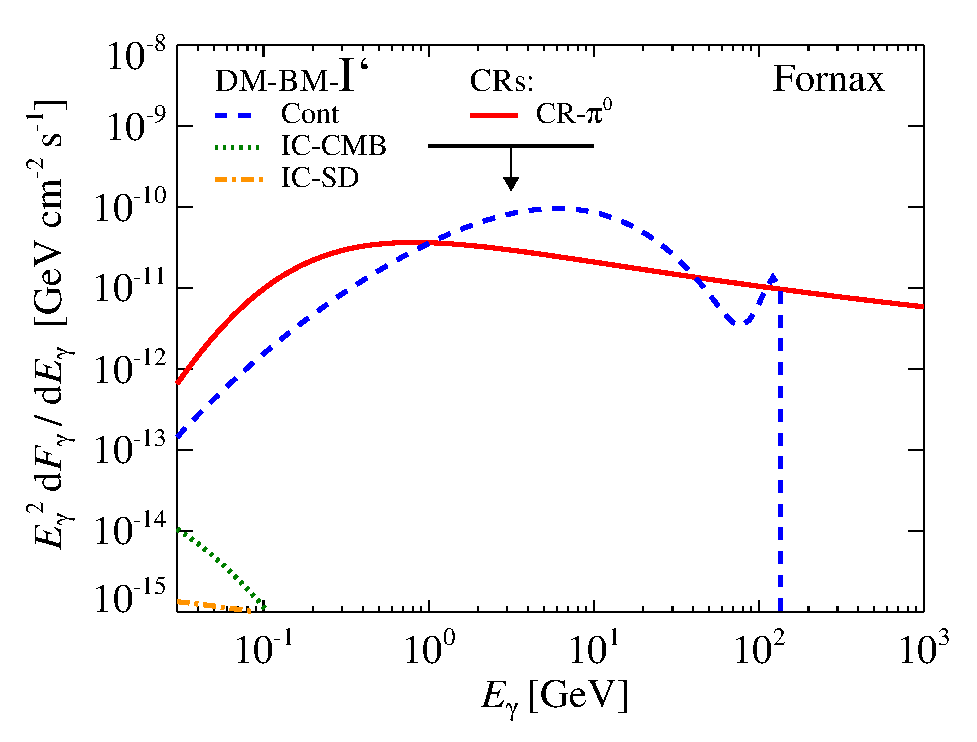
\includegraphics[width=0.49\columnwidth]{figures/flux.BMcompI.v13.0.1deg.1.6T.SubMass.IR2.noMW.woGal.eps}
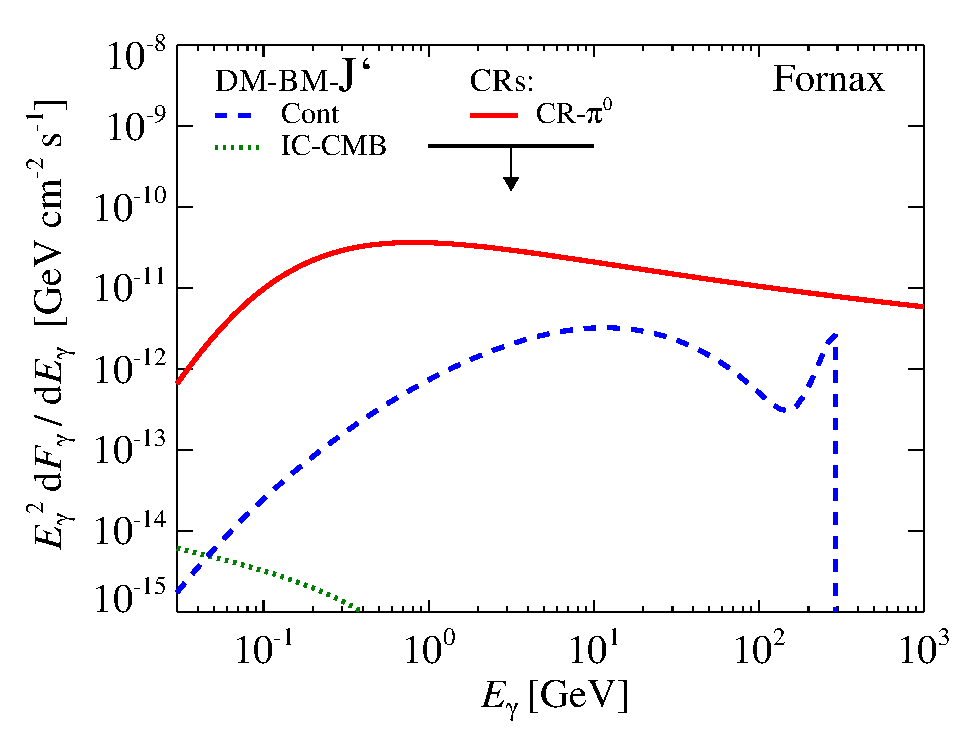
\includegraphics[width=0.49\columnwidth]{figures/flux.BMcompJ.v13.0.1deg.1.6T.SubMass.IR2.noMW.woGal.eps}
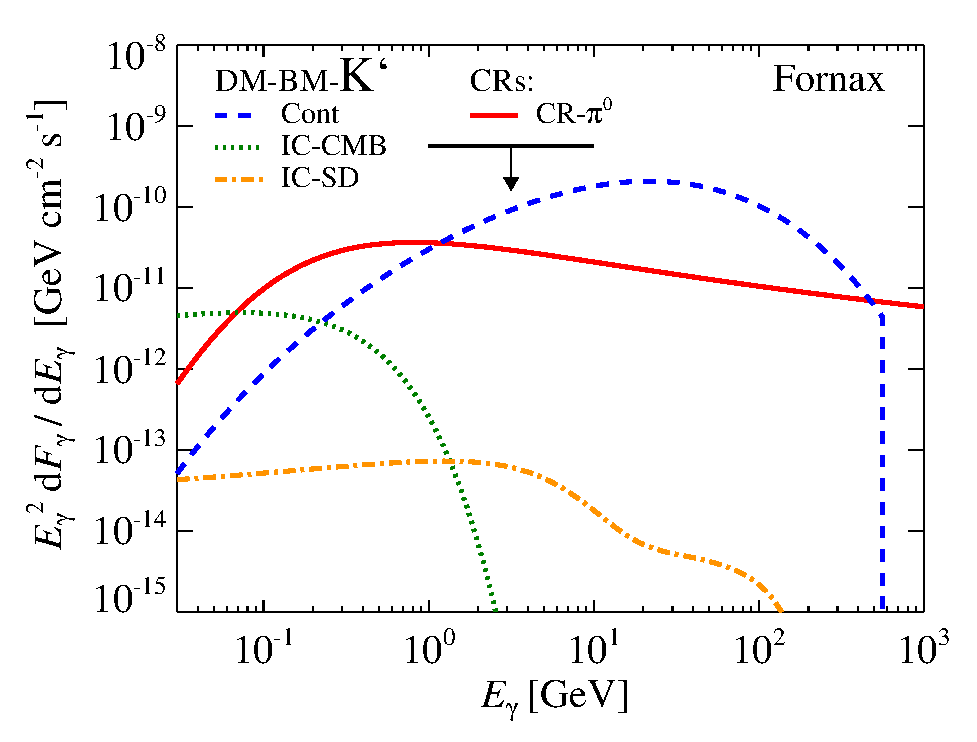
\includegraphics[width=0.49\columnwidth]{figures/flux.BMcompK.v13.0.1deg.1.6T.SubMass.IR2.noMW.woGal.eps}
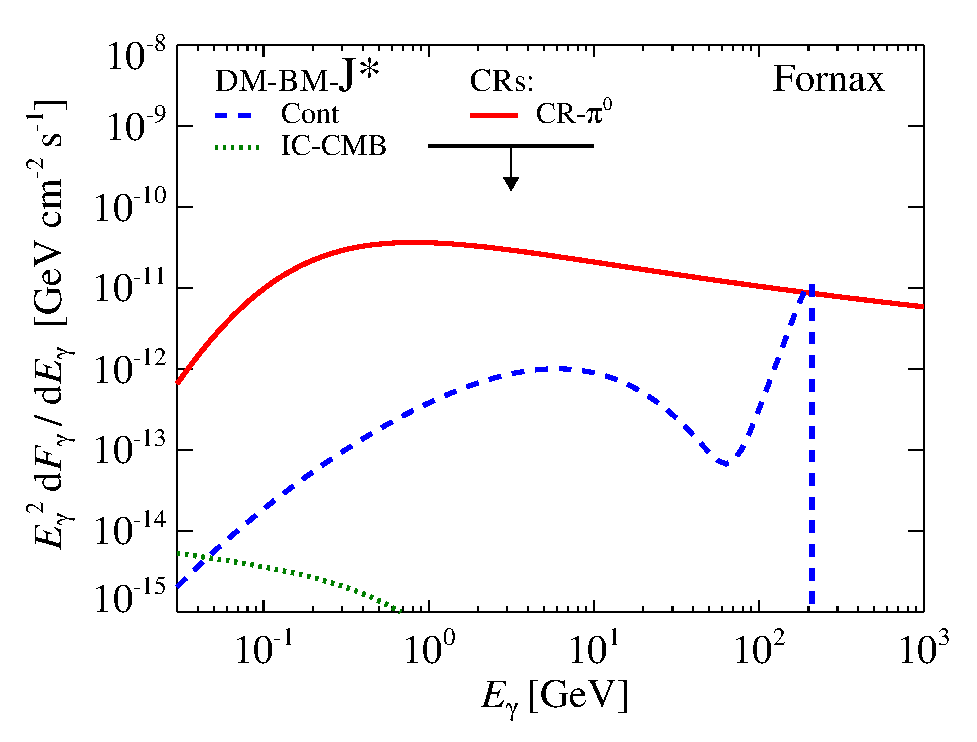
\includegraphics[width=0.49\columnwidth]{figures/flux.BMcompJs.v13.0.1deg.1.6T.SubMass.IR2.noMW.woGal.eps}
\caption{\it Comparing the differential flux from different models: we
  show the continuum emission from DM benchmark (BM) models (blue
  dashed), electrons and positrons from DM BM models that
  Compton-upscatter CMB photons (green dotted) as well as dust and
  star photons (orange dash-dotted), and CR induced gamma-ray emission
  (red solid). Each panel is associated with an individual DM BM
  model; upper left $\Ip$, lower left $\Kp$, upper right $\Jp$, and
  lower right $\Js$. The emission is calculated for the Fornax cluster
  using a point spread function of $0.1\deg$. The substructures boost
  the gamma-ray flux from IC upscattered CMB and continuum emission by
  a factor of 730 while the IC upscattered SD photons are only boosted
  by 20. Extended upper limits from Fermi-LAT after 18 months \protect
  \cite{2010ApJ...717L..71A} are also shown. \C{We find it hard to
    detect even the brightest BM models, $\Ip$ and $\Kp$, where the
    continuum emission is dominating the total emission in the
    GeV energy range.}}
 \label{fig:diff_BM}
\end{minipage}
\end{figure*}

For the LP DM models, however, the main contributions
to the expected extended gamma-ray flux is coming from the IC
upscattered photons on various photon background fields. Depending on
the spatial and spectral distribution of electrons and positrons as
well as the photon background fields, the resulting spectral
distributions of gamma-rays can differ greatly. Hence it is interesting
to understand which spectral features and energy regimes are
dominating.

If the enhancement due to substructures in clusters is significant,
then the distribution of electrons and positrons follows the radial
profile of substructures outside the cluster center where the smooth
DM density profile is dominating. In addition, the cooling of the
steady state electron and positron distribution is dominated by SD
photons in the center. Especially since the SD distribution is
centrally peaked and the substructure distribution peaks in the
outskirts around $\rvir$, the overlap between electrons/positrons and
SD photons is small. This results in a suppression of the IC
upscattered SD photons relative to the IC upscattered CMB photons, the
final state radiation, and the continuum emission. However, if
substructures are only marginally dominating over the smooth
distribution in a cluster, the SD component becomes relatively more
important.

In Fig.~\ref{fig:IR_comp} we show the total IC emission as well as its
individual contributions from different IC upscattered radiation
fields. The left panel shows the gamma-ray emission from the LP model
and the right panel from the $\Kp$ BM model, and for comparison we
overplot the emission expected from the CRs. Due to the flat electron
and positron spectrum resulting from the LP DM model and the smaller
mean energy of the CMB compared to the SD, we find that the
upscattered CMB photons dominate the total DM IC emission in the
energy regime below 100~GeV, while the SD dominate above this
energy. For the BM models, this transition energy is shifted towards
smaller energies since the electron and positron spectrum has a
steeper spectral distribution (see Fig.~\ref{fig:q_DM}). At the
highest gamma-ray energies of about 100~GeV and above, the IC from
starlight steepens because it probes the high energy tail of the
electrons and more importantly, it suffers from the Klein-Nishina
suppression. When substructures are present, most of their flux
resides in the outer parts of clusters. However, if we remove the
boost from substructures, the density profile of electrons and
positrons is more centrally peaked, and the relative importance of the
IC upscattered SD increases by a factor $\sim 30$ \footnote{\C{Note
    that for the leptophilic DM model this increase is much smaller
    since Sommerfeld enhancement is no longer dominated by the low
    velocity DM particles living in the subhalos (see
    Sect.~\ref{sect:LP} for more details.}}.  A larger fraction of
electrons (in the core) will now also cool by Compton-upscattering SD
photons which suppresses the IC-upscattered CMB light.  For
comparison, we include the contribution of IC upscattered SD photons
and to bracket the uncertainty in the SD model, with a smaller amount
of dust. In this low-dust model, we have reduced the energy in dust by
a factor 10. However, the resulting flux from the IC upscattered dust
in this model only decreases with a factor that is slightly smaller
than 10 since the IC cooling of the electrons and positrons also
decreases.

Because of the large total boost factor for the LP model ($\sim5\times
10^5$), we overproduce the upper gamma-ray limit in the $1-10$~GeV
energy interval set by Fermi-LAT by about a factor 50. This strongly
constrains the boost from both substructures and the
SFE. Additionally, these constraints might improve with future more
sensitive Cherenkov telescopes such as CTA. However, considering that
an indirect detection of DM in clusters relies on the boost from
substructures whose main contribution comes from the periphery, we
conclude that the wide angular extent of clusters on the sky in
gamma-rays suggest that these sources are not ideal for Cherenkov
telescopes since their sensitivity drops linearly with source
extension.

\begin{figure*}
\begin{minipage}{2.0\columnwidth}
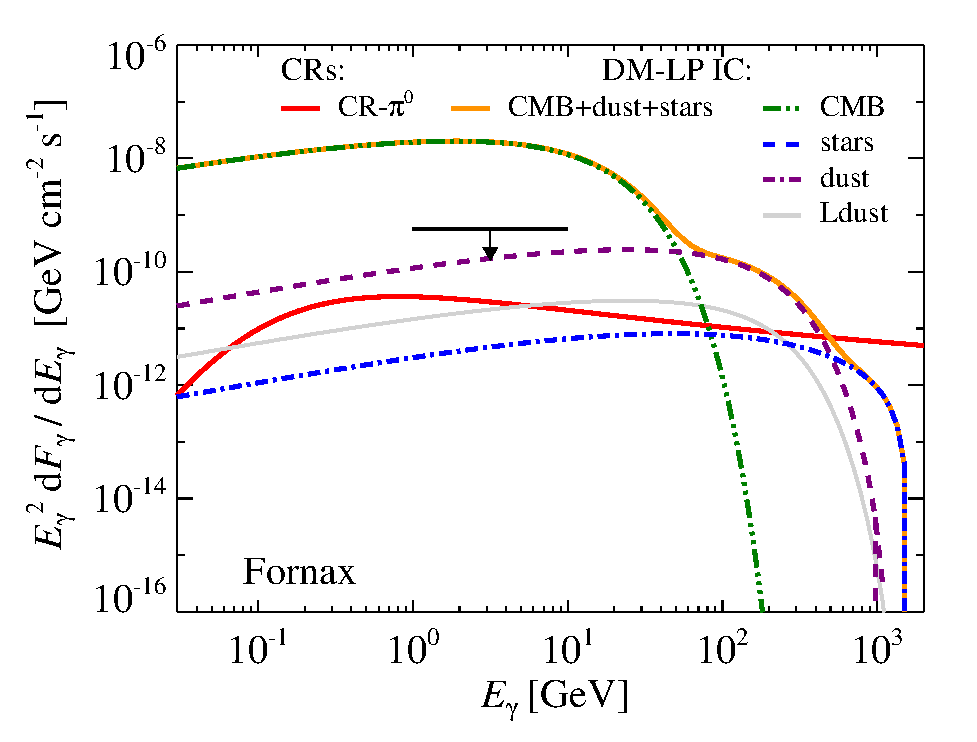
\includegraphics[width=0.49\columnwidth]{figures/flux.IRcomp.v13.0.1deg.1.6T.SubMass.elmu.SF700.noMW.woGal.eps}
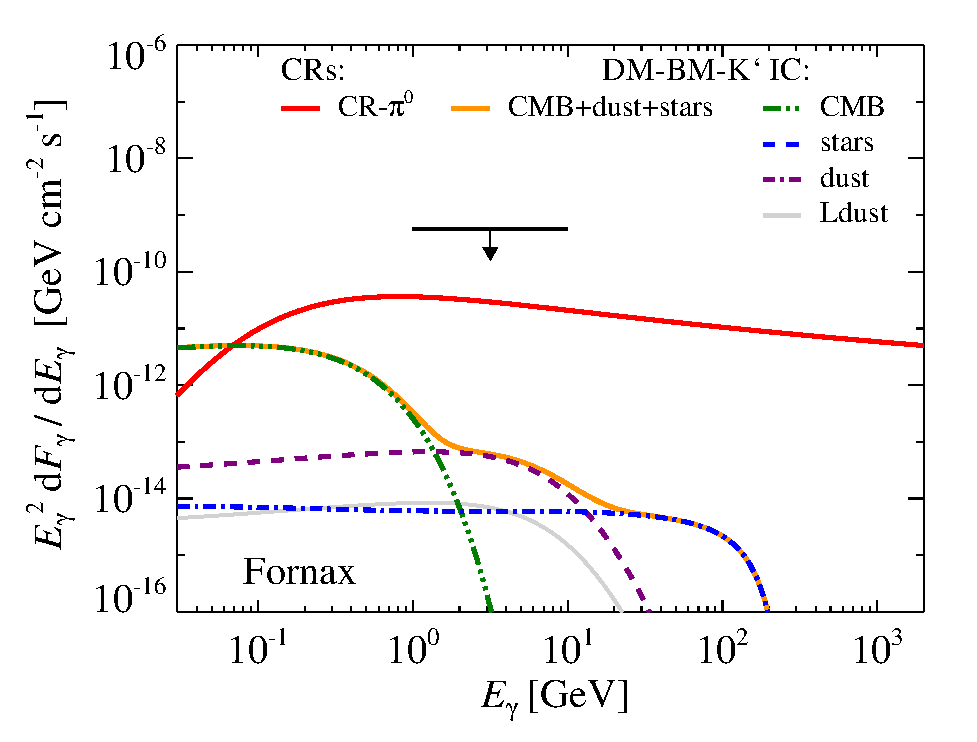
\includegraphics[width=0.49\columnwidth]{figures/flux.IRcomp.BMv13.0.1deg.SubMass.noMW.woGal.eps}
\caption{\it Comparing the flux from different inverse Compton
  upscattered radiation fields. We show the differential inverse
  Compton emission induced by leptophilic DM in the left panel and by
  the $\Kp$ benchmark model in the right panel. The contribution from
  each individual radiation field from top line to bottom line; CMB
  (green dashed-triple-dotted), dust (purple dashed), stars (blue
  dashed-dotted). The sum of the three components are shown with the
  orange solid line. The red solid lines show the CR induced gamma-ray
  flux. The black arrow shows the spatially extended differential
  upper limit from Fermi \protect \cite{2010ApJ...717L..71A}
  indicating that the LP model assumptions such as Sommerfeld and/or
  substructure boost are in conflict with the upper limit. \del{We
    also show projected CTA point source sensitivities ($5\sigma$,
    50h).}  All fluxes are calculated for the Fornax cluster within
  $\rvir$ using a point spread function of $0.1\deg$. \C{For this
    cluster, the enhancement due to substructures from IC upscattered
    CMB and SD photons is 730. The Sommerfeld boost is 530.}}
 \label{fig:IR_comp}
\end{minipage}
\end{figure*}

It is also interesting to compare the total contribution from the LP
model, the brightest BM model ($\Kp$), and the CR induced emission. In
Fig.~\ref{fig:flux_int} we show the integrated flux from Fornax for
our different gamma-ray models and compare it to the unresolved
integrated flux upper limit on Fornax set by Fermi-LAT where they
averaged the flux over the energy range $0.2-100\,\gev$ assuming a
spectral index of 2. Again, the annihilation flux in the LP model is
in conflict with the upper limits by Fermi-LAT, although only by a
factor of 10 which is about a order magnitude less constraining than
the differential flux in the energy range $1-10$~GeV. As shown in this
figure, the LP model is dominating the entire gamma-ray energy range
up to the DM rest mass energy in this model of about 1~TeV. Finally,
we note that the flux the DM BM $\Kp$ model is larger than the
predicted emission from the CRs in the $1-100$~GeV energy
regime. \C{Hence, for an experiment with a high sensitivity even for
  for extended sources, the prospects for detecting the $\Kp$ BM model
  over the expected gamma-ray background induced by CRs looks
  promising in clusters. Present day Cherenkov telescopes, however,
  have a trigger region that is smaller than the size of clusters,
  hence it has to be increased to several degrees to overcome problems
  with background estimation. In addition, even though the projected
  CTA point source sensitivity ($5\sigma$, 50h) shows the potential of
  this experiment in constraining leptophilic models as well as BM
  models with a very large neutralino mass $m_\chi c^2 \gtrsim 1$~TeV,
  we find that analysis techniques have to be developed that enable
  the detection of extended sources without too much degradation of
  sensitivity.}

\begin{figure}
 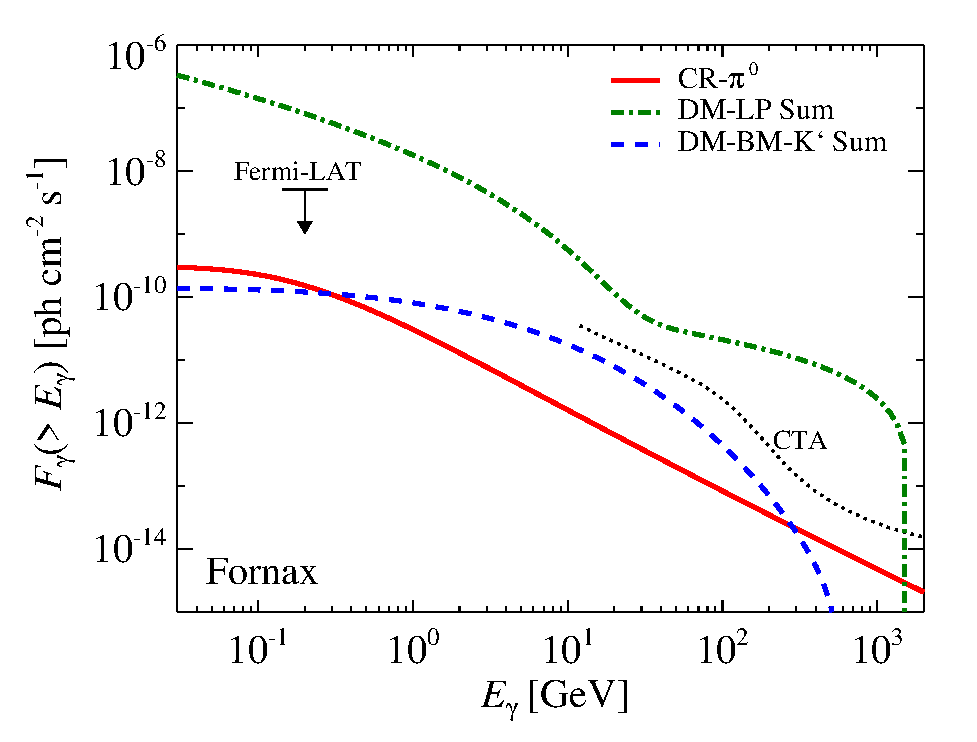
\includegraphics[width=0.99\columnwidth]{figures/flux.int.v13.0.1deg.1.6T.SubMass.SF700.IR2.noMW.woGal.eps}
 \caption{\it Comparing the energy integrated flux from different
   models. We show the emission from CR induced emission (red solid),
   a leptophilic (LP) model that includes both final state radiation
   and IC upscattered CMB, dust and starlight (green dash-dotted), and
   the benchmark $\Kp$ model (BM) that includes continuum emission,
   and IC upscattered CMB, dust and starlight (blue dashed). The black
   arrow shows the spatially extended integrated flux upper limit set
   by Fermi-LAT again indicating challenges for the assumptions
   underlying the LP model. We also show projected CTA point source
   sensitivities ($5\sigma$, 50h). The emission is calculated for the
   Fornax cluster using a point spread function of $0.1\deg$. The
   boost from Sommerfeld and substructures is about 530 and 730,
   respectively.}
 \label{fig:flux_int}
\end{figure}

We continue by comparing the estimated differential flux from Fornax
to three other clusters in Fig.~\ref{fig:clu_comp}; the close-by and
well studied Virgo cluster, the X-ray bright Perseus clusters, and the
massive merging Coma cluster. We find high DM induced gamma-ray fluxes
from the Fornax and Virgo clusters, which highlight them as promising
targets for indirect DM searches. \C{Especially in the $1-10$~GeV
  energy range it is quite striking how constraining the upper limits
  are for some of the clusters. At these energies, Fermi-LAT has its
  peak sensitivity due to a combination of increasing effective area
  and decreasing source spectra as a function of energy. The upper
  limits for Virgo and Perseus are unfortunately background
  contaminated by AGN activity from M87 and NGC 1267, respectively,
  and do not gain much from the increased sensitivity. In addition,
  the angular radius of Virgo is about 6 degrees, while the extended
  upper limit from Fermi-LAT is calculated assuming a $\sigma=1.2$
  degree radius. In fact, the ratio of the virial radius to the
  assumed extension for the upper limits $\rvir/\sigma$ for $($Fornax,
  Coma, Virgo$)$ are $(2.8,\,1.6,\,5.3)$, respectively. Similarly, it
  is interesting to compare the radius that contain 68\% of the flux
  to the assumed extension, $r_{68}/\sigma$, which is given by
  $(1.7,\,1.0,\,3.3)$ for $($Fornax,Coma,Virgo$)$, respectively. This
  further motivates a re-calculation of the Fermi upper limits to
  account for the full extension of the galaxy clusters.}  \del{Note,
  however, that we have used spatially unresolved upper limits, which
  is quite optimistic for the Virgo cluster which has an angular
  extended of 7 degrees. It is quite striking how constraining the
  upper limits are for the Fornax cluster are compared to the other
  clusters, especially in the $1-10$~GeV energy regime.}  \C{We also
  find that the high CR-induced flux in Coma and Perseus is making it
  difficult for indirect DM searches in those clusters if the boost
  factors are much lower than assumed in this work.} \del{is of the
  same magnitude as the DM flux from LP models, making it difficult
  for indirect DM searches in those clusters.} Conversely, the Fornax
cluster is a great target for indirect DM studies because the relative
low gamma-ray flux from CRs, absents of an active AGN, and high DM
gamma-ray flux. \del{The Fermi-LAT three-year data will be able to
  constrain the smallest mass of substructures using the DM BM
  models.}

What is the figure of merit for selecting the most promising cluster
targets for indirect DM searches? To this end, we employ the
luminosity-to-mass scaling relations. The gamma-ray luminosity from
the smooth density profile is given by \cite{2009PhRvL.103r1302P}
\begin{equation}
L_{\gamma,\sm} \propto \int \dd V \rho(r)^2 \propto \frac{M_{200}\,c^3}
{\left[\log\left(1+c\right)-c/(1+c)\right]^2} \propto \mvir^{0.83}\,,
\end{equation}
\del{and the total DM luminosity that includes boost factors for the LP and
the BM models are given by}
%\begin{eqnarray}
%\label{eq:LP_scaling}
%L_{\gamma,\rmn{LP}} &=& L_{\gamma,\rmn{smLP}} \B_\rmn{LP} \propto \frac{\mvir^{0.73}}{D_\rmn{lum}^2},\\
%\label{eq:BM_scaling}
%L_{\gamma,\rmn{BM}} &=& L_{\gamma,\rmn{smBM}} \B_\rmn{BM} \propto  \frac{\mvir^{1.06}}{D_\rmn{lum}^2},\\
%\B_\rmn{LP}&=&\B_\sfe \B_\sub \propto \mvir^{-1/3}\mvir^{0.23} \propto
% \mvir^{-0.1}\,,\\
%\B_\rmn{BM}&=&\B_\sub \propto \mvir^{0.23}\,.
%\end{eqnarray}
\del{Hence, increasing the cluster mass in the BM model by a factor two
more than doubles the luminosity, but increasing the luminosity
distance, $D_\rmn{lum}$, by a factor two decrease the flux by a factor
four. We note that the IC from upscattered SD photons scales slightly
softer with mass, hence gives rise to a larger fraction of gamma-rays
in low mass clusters compared to the total gamma-ray flux.}
\C{and the total DM luminosity that includes boost factors for the LP and
the BM models is given by
\begin{eqnarray}
\label{eq:DM_scaling}
L_{\gamma} &=& L_{\gamma,\rmn{sm}} \B_\rmn{sub} \propto \frac{\mvir^{1.06}}{D_\rmn{lum}^2},\\
\rmn{where} & &\B_\sub \propto \mvir^{0.23}\,.
\end{eqnarray}
Hence, increasing the cluster mass by a factor two more than doubles
the DM luminosity, but increasing the luminosity distance,
$D_\rmn{lum}$, by a factor two decrease the flux by a factor four. We
note that the IC from upscattered SD photons scales slightly softer
with mass, hence gives rise to a larger fraction of gamma-rays in low
mass clusters compared to the total gamma-ray flux. Also note that we
have not included the SFE for the LP model in
Eq.~(\ref{eq:DM_scaling}) since it saturates to a constant value in
the substructures. However, if only a small fraction of the DM resides
in the subhalos, the scaling of the LP DM becomes slightly steeper due
to the mass dependence inferred from the velocity dispersion:
\begin{eqnarray}
L_{\gamma,LPnosub} &=& L_{\gamma,\rmn{sm}} \B_\rmn{sfe} 
\propto \frac{\mvir^{0.5}}{D_\rmn{lum}^2},\\
\rmn{where} &\quad&\B_\rmn{sfe} \propto \mvir^{-1/3}.
\end{eqnarray}}


\begin{figure*}
\begin{minipage}{2.0\columnwidth}
 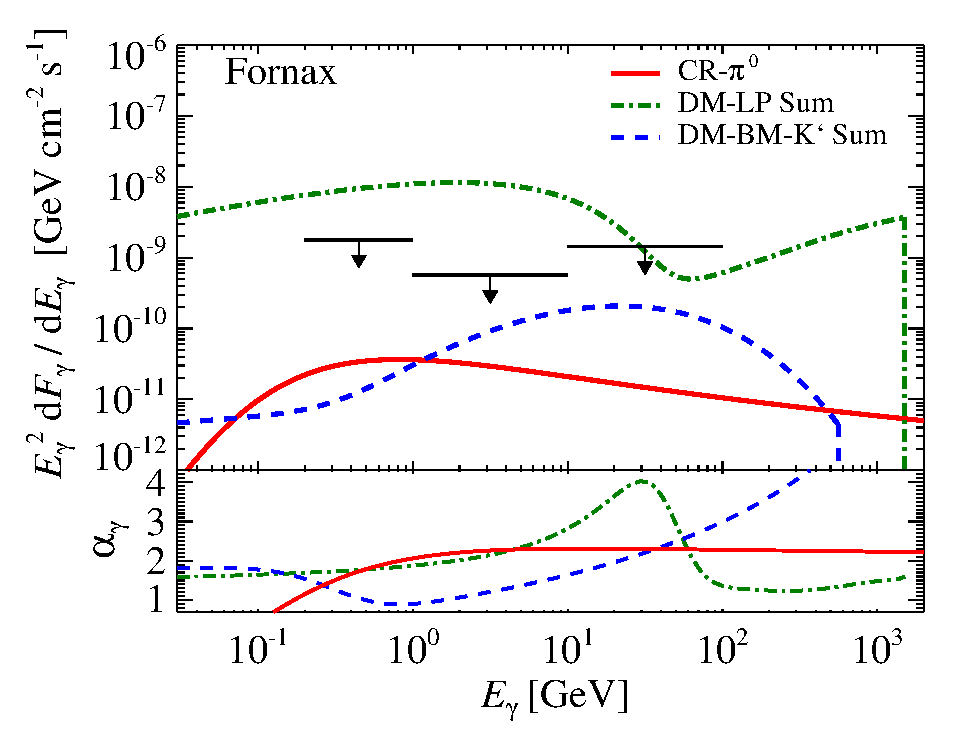
\includegraphics[width=0.49\columnwidth]{figures/flux.cluster.Fornax.v13.0.1deg.1.6T.SubMass.SF700.IR2.noMW.woGal.eps}
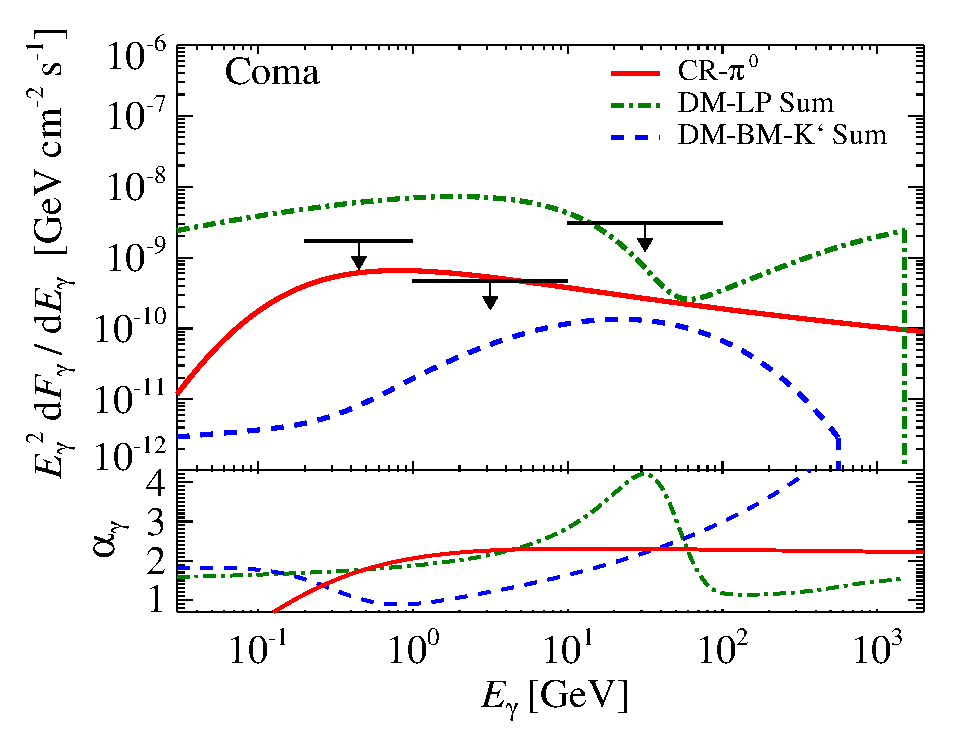
\includegraphics[width=0.49\columnwidth]{figures/flux.cluster.Coma.v13.0.1deg.1.6T.SubMass.SF700.IR2.noMW.woGal.eps}
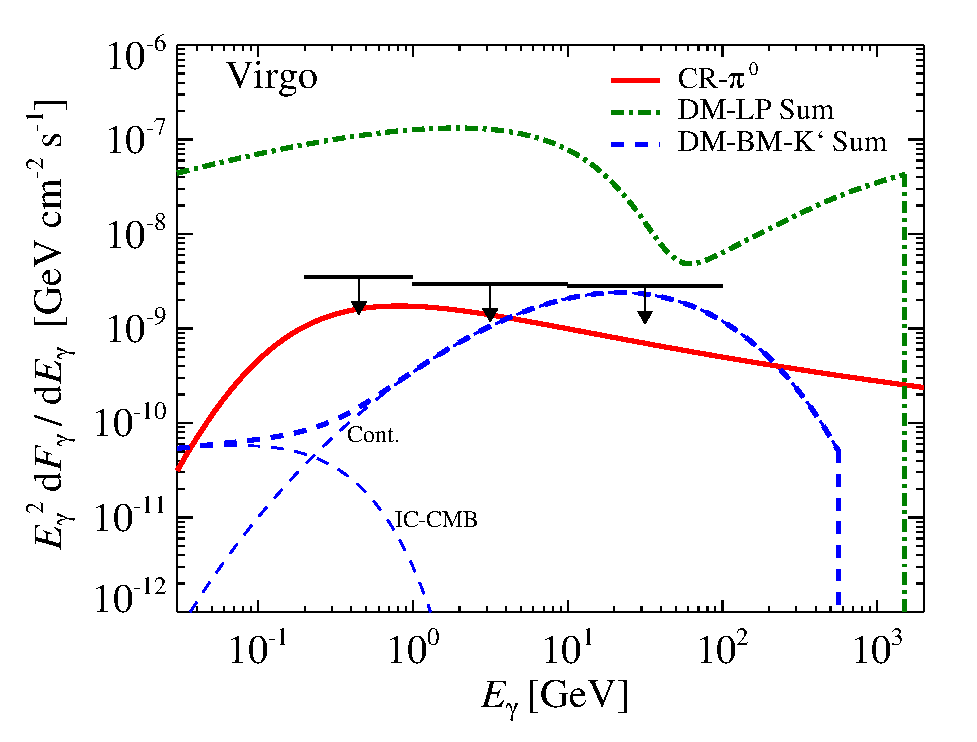
\includegraphics[width=0.49\columnwidth]{figures/flux.cluster.Virgo.v13.0.1deg.1.6T.SubMass.SF700.IR2.noMW.woGal.eps}
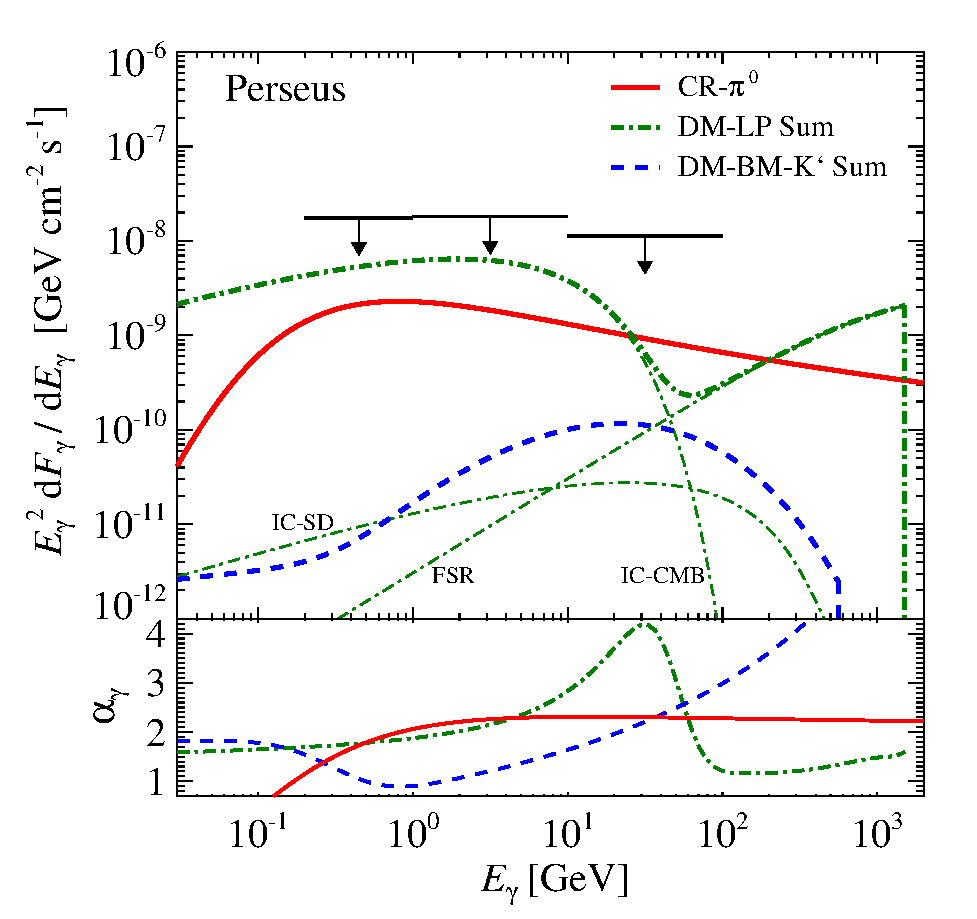
\includegraphics[width=0.49\columnwidth]{figures/flux.cluster.Perseus.v13.0.1deg.1.6T.SubMass.SF700.IR2.noMW.woGal.eps}
\caption{\it Comparing the gamma-ray emission from different
  clusters. We show the differential flux of clusters \C{in the upper
    panel of each figure}: Fornax (upper left), Coma (upper right),
  Virgo (lower left), and Perseus (lower right). We show CR induced
  emission (red solid), a leptophilic (LP) model that includes both
  final state radiation and IC upscattered CMB, dust and starlight
  (green dash-dotted), and the benchmark $\Kp$ model (BM) that
  includes continuum emission, and IC upscattered CMB, dust and
  starlight (blue dashed). The arrows show the spatially extended
  differential upper limits set by Fermi-LAT in the energy ranges
  $0.2-1$~GeV, $1-10$~GeV, and $10-100$~GeV from left to right. We
  show the individual components for the BM model and LP model for
  Virgo and Perseus, respectively. \C{In the lower panel of each
    figure we show differential spectral indices, $\alpha_\gamma$,
    where $\dd F_\gamma/\dd E_\gamma \sim E_\gamma^{-\alpha_\gamma}$.}
  The flux from the clusters is integrated out to $\rvir$ using a
  point spread function of $0.1\deg$ and includes the boost from
  substructures. We find that the lower GeV energy regime is most
  constraining due to the peak sensitivity of Fermi at these energies
  and use this regime to get upper limits on boost factors.}
 \label{fig:clu_comp}
\end{minipage}
\end{figure*}

\C{For consistency we provide in addition the differential spectral
  indices $\alpha_\gamma=-\frac{\dd \log(\dd F/\dd E)}{\dd \log(E)}$
  for the different emission models in the lower panels of
  Fig.~\ref{fig:clu_comp}. We find very similar spectral indices for
  different clusters when the boost from substructures is substantial,
  while for models without substructures the relative contribution
  from the upscattered dust and starlight breaks the spectral
  universality for the DM models. In the $1~\gev-1~\tev$ energy regime
  the CR spectral index is approximately constant $\sim (2.1-2.3)$,
  while the spectral index for the LP model has a large spread and
  varies between $1.2-4.0$, hence implying that gamma-ray upper limits
  are more sensitive to the specific energy regime for these
  models. Similarly, the index for the BM $\Kp$ model is about 1.0 at
  1~GeV and increases monotonically for higher energies, which also
  suggests that the flux upper limits contrasted to this model are
  sensitive to the specific energy range, and where a small energy
  range would be preferred. In experiments is the spectral index often
  fixed over an energy range, hence we show in
  Tab.~\ref{tab:spectral_index} the indices for our emission models in
  four different energy bands. We find that these spectral indices
  have a much smaller spread, hence reducing the importance of the
  specific energy regimes. For further discussion about the impact of
  different spectral indices on the gamma-ray upper limits see
  Eq.~(\ref{sect:spectral}) and related text.}

\begin{table}
\begin{tabular}{ccccc}
\hline\hline
      Model & $\alpha_{100\,\rmn{MeV}}^{1\,\rmn{GeV}}$  & 
              $\alpha_{1\,\rmn{GeV}}^{10\,\rmn{GeV}}$   & 
              $\alpha_{10\,\rmn{GeV}}^{100\,\rmn{GeV}}$ &
              $\alpha_{100\,\rmn{GeV}}^{1\,\rmn{TeV}}$  \\
\hline
CR-$\pi^0$      & 1.44 & 2.24 & 2.30 & 2.26 \\
DM-LP Sum       & 1.74 & 2.20 & 3.06 & 1.30 \\
DM-BM-$\Kp$ Sum  & 1.28 & 1.22 & 2.23 & -    \\
\hline\hline
\end{tabular}
 \caption{\C{Gamma-ray spectral indices $\alpha_{E_1}^{E_2}$ between
     energies $E_1$ and $E_2$. We show the spectral index for three
     different emission models where the boost from substructures is
     included; the CR induced emission, the leptophilic (LP) model
     that includes both final state radiation and IC upscattered CMB,
     dust and starlight, and the benchmark (BM) $\Kp$ model that
     includes continuum emission, and IC upscattered CMB, dust and
     starlight. The indices are derived for the Fornax cluster,
     although the variance between clusters is very small when the
     enhancement from substructures is included which suppresses the
     relative contribution from the upscattered dust and starlight
     component that is cluster dependent. \label{tab:spectral_index}}}
\end{table}

In this section, we have found that the LP DM models overproduces both
the spatially extended differential and integrated gamma-ray flux
upper limits set by the Fermi-LAT 18 month data for several
clusters. We can use these upper limits to constrain the boosts due to
SFE and substructures. Furthermore, as more sensitive experiments and
better upper limits emerge, we can start ruling out models that give
rise to boost factors that are manifested in the gamma-ray flux. It is
especially interesting to constrain the SFE, where a boost of the
particle physics cross section of 300 is required to explain the
excess of electrons and positrons observed in the vicinity of Earth by
PAMELA/Fermi/HESS. In Fig.~\ref{fig:boost_const} we use the estimated
flux \C{within $\rvir$ of four bright and maximal constraining
  clusters (Fornax, M49, Norma, and Coma, where we have excluded Virgo
  due to its large angular extent) to limit} the SFE as well as the
minimum mass of substructures where
$M_\rmn{lim}\propto\mvir^{0.226}$. We find that M49 and the Fornax
cluster are the most constraining clusters, although the current upper
limits are not good enough to rule out the boost from substructures or
SFE. Assuming that the PAMELA positron excess is due to SFE DM, then
in order not to overproduce the differential upper limits set by
Fermi-LAT in the energy range\footnote{We average the LP DM flux in
  the energy range $1-10$~GeV before we compare it to the upper
  limits.}  $1-10$~GeV, we can constrain the smallest mass of
substructures to $M_\rmn{lim}\gtrsim 10\,\msun$. Instead assuming the
standard mass of the smallest substructures of $M_\rmn{lim}\approx
10^{-6}\,\msun$, we can constrain the \C{saturated boost from SFE to
  about 14 in M49 and 22 in Fornax, which corresponds to a maximum SFE
  in the MW of about 8 and 13, respectively. Hence, we conclude that
  without substantial improvement in the modelling of these extended
  sources, Fermi-LAT will not be able to rule out LP models in their
  current form using clusters.} \del{Note that after about six years
  of observations with Fermi-LAT, we will be able to rule out the LP
  model assuming a substructure boost with a smallest mass of
  $M_\rmn{lim} \approx 10^{-6}\,\msun$.}

\begin{figure}%[t]
 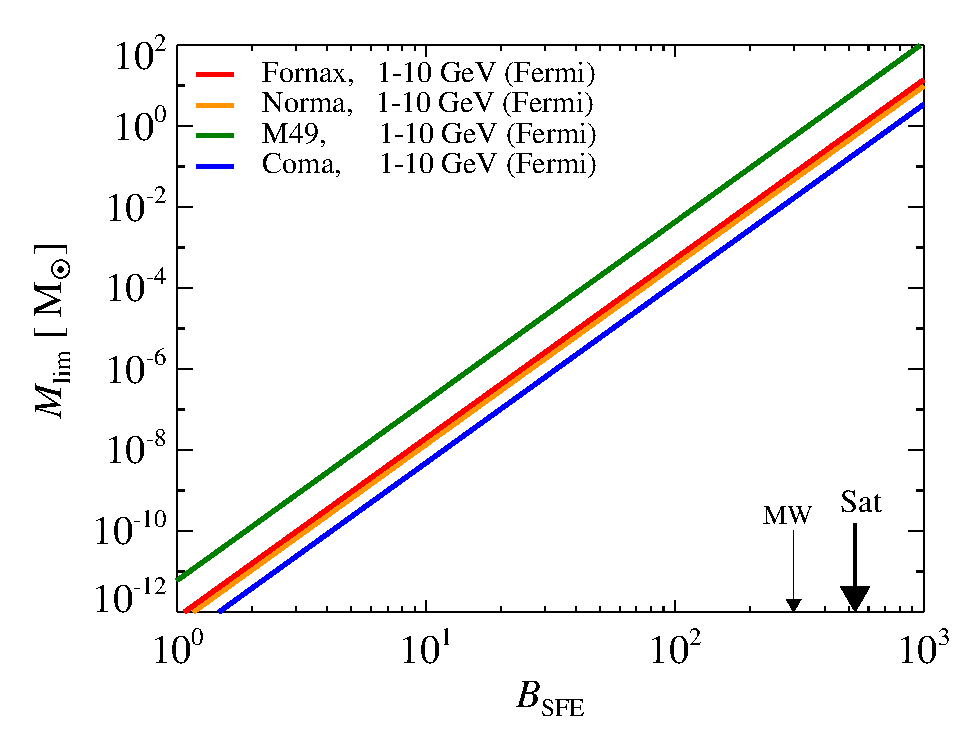
\includegraphics[width=0.99\columnwidth]{figures/LP.const.diff.v13.0.1deg.1.6T.SubMass.SF700.IR2.noMW.woGal.eps}
 \caption{\it Constraining boost factors using flux upper limits. The
   leptophilic (LP) gamma-ray emission is derived within $\rvir$ using
   a point spread function of $0.1\deg$. In order not to overproduce
   the Fermi-LAT differential flux upper limits in the energy interval
   $1-10$~GeV the boost from substructures and Sommerfeld enhancement
   (SFE) is constrained for four clusters; Fornax (red), Norma
   (orange), M49 (green), and Coma (blue). \C{We indicate both the
     saturated SFE of 530 (right black arrow) as well as the the local
     boost in the Milky Way of 300 (c.f. Eq.~\ref{eq:B_sfe}) that is
     required to explain the electron and positron excess observed at
     Earth with LP DM (left black arrow). If the DM interpretation is
     correct, we can constrain the smallest size of halos to be larger
     than $10\,\msun$. Contrarily, if the smallest size of DM halos is
     $10^{-6}\,\msun$, we can constrain the SFE to about 14 in M49 and
     22 in Fornax. This corresponds to a maximum SFE in the MW of
     about 8 and 13, respectively, which would be too small to support
     the DM annihilation hypothesis for the PAMELA/Fermi excess.}}
 \label{fig:boost_const}
\end{figure}


\section{Surface brightness profiles}
\label{sect:spatial}

The large angular extent of clusters on the sky in combination with
the small PSF of most gamma-ray probes ($\sim 0.1$~deg) suggest that
we would be able to probe the different spatial regimes of a
cluster. Especially important is the spatial distribution of the
gamma-ray emission as it biases upper limits derived for spatially
extended clusters where a simple profile is often assumed. In fact, we
will show that if DM substructures are present with the discussed
abundances, the gamma-ray brightness profile is almost flat and very
different from the gamma-ray distribution following a smooth density
profile with a steep outer surface brightness slope of $-5$.

In this section we investigate the gamma-ray surface brightness
profiles induced by both CRs and different models of DM in more
detail. We start by comparing the intrinsic surface brightness that
includes substructures from different clusters in
Fig.~\ref{fig:SB_clu}. As expected, we find that the DM flux in all
clusters follows the same universal shape imposed by the
substructures. Already at $0.01\rvir$, we are dominated by the
substructures due to the projection of their peaked distribution the
outer cluster regions (see Sect.~\ref{sect:subst} for a longer
discussion). This implies that the spatial distribution of
annihilating DM is independent of the type of DM model, and can not be
used to separate different models. The surface brightness, $S_\gamma$,
of the DM scales as $S_\gamma\propto\bsub L_{\gamma} \mvir^{-2/3}
\propto \mvir^{0.59}$, which explains the factor three difference in
normalization between the most massive cluster Coma and the least
massive cluster Fornax with a mass ratio of about 10. \del{The flux
  from the LP model shows a smaller spread in the normalization which
  is due to the additional contribution from SFE with a negative mass
  trend, hence a flux normalization with a softer mass-scaling of
  $S_\gamma\propto\mvir^{0.06}$.} The surface brightness induced by
CRs is proportional to the projected squared gas profile with an
additional enhancement in the center of cool core clusters due to the
adiabatic compression of CRs during the formation of the cool
core. Hence, we see a much larger variation in these profiles driven
by the large variation of the gas mass fraction. It is noticeable that
Fornax shows such a small surface brightness. This is explained by the
low gas density outside the BCG and the less abundant CR population in
a small cluster compared to a massive cluster
\cite{2010MNRAS.409..449P}.  This is the reason why Fornax is such a
good target for indirect DM searches, and superior to DM searches in
dwarf galaxies.

\begin{figure}
 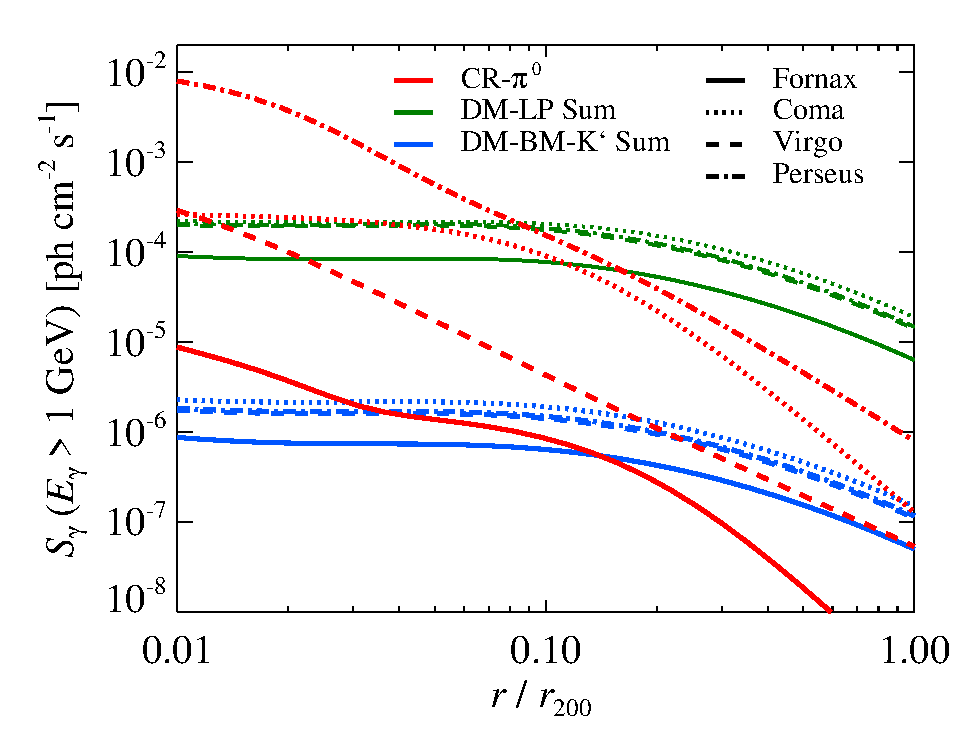
\includegraphics[width=0.99\columnwidth]{figures/SB.v13.1GeV.SF700.SubMass.elmu.eps}
 \caption{\it Comparing the intrinsic surface brightness from
   different clusters without taking PSF effects into account. We show
   the CR induced emission (red), leptophilic emission (green), and
   emission from the $\Kp$ benchmark model (blue). The different line
   styles each represent a cluster; Fornax (solid), Coma (dotted),
   Virgo (dashed), and Perseus (dash-dotted). We include the boost
   from both substructures and Sommerfeld effect. Notice the very
   similar shape and normalization of the DM models, while the CRs
   have a much larger scatter in the profiles due to the large
   variation of the gas fraction in these clusters.}
 \label{fig:SB_clu}
\end{figure}

To quantify the impact of substructures on the spatial profiles in
more detail we again turn to the Fornax cluster and show in
Fig.~\ref{fig:SB_sub} a comparison of surface brightness profiles with
and without substructures. It is quite remarkable how flat the
profiles become when substructures are present compared to the case
without. This implies that the relative flux within the PSF in the
center is comparable to the outer parts, which should increase the
signal-to-noise significantly. If we assume that -- for
some reason -- substructures are suppressed in the Fornax cluster, then the expected
signal from DM is swamped by astrophysical backgrounds over the entire
extent of the cluster, even though Fornax has one of the highest
ratios of DM to CR induced gamma-ray brightness.

\begin{figure}%[t]
 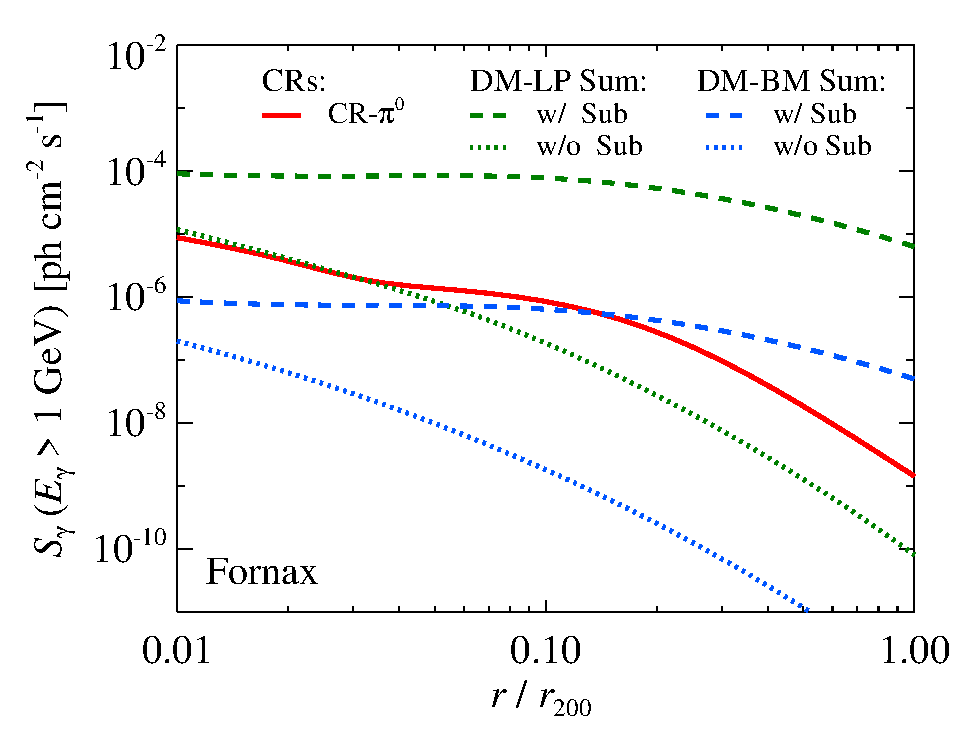
\includegraphics[width=0.99\columnwidth]{figures/SB.resolved.v13.1GeV.SF700.noSuB.vs.SubMass.elmu.eps}
 \caption{\it The impact of substructures on the intrinsic surface
   brightness profile o the Fornax cluster at 1~GeV. The emission
   induced by CRs is denoted by the red solid line, the leptophilic
   model by green lines, and the DM $\Kp$ benchmark model by blue
   lines. The dashed lines show the brightness profiles where the
   boost from substructures is included while the substructures are
   excluded for the dotted lines. The boost from Sommerfeld
   \C{enhancement with and without substructures is 130 and 530
     respectively, where in addition the boost due to substructures is
     about 730.} Notice the nearly flat profiles when substructures
   are included, and the relative large boost at $0.01\rvir$ that is
   due to projection of peripheral substructures onto the cluster
   center.}
 \label{fig:SB_sub}
\end{figure}

In order to learn about the spatial distribution of the DM flux in
various clusters for different DM models and the associated gamma-ray
components, we show in the left panel of Fig.~\ref{fig:SB_clu_nosub}
the brightness profiles for the smooth DM distribution for the same
four representative clusters that were shown previously in
Fig.~\ref{fig:SB_clu}.  We find that the surface brightness,
$S_\gamma$ of the DM emission above 1~GeV in the outer parts of all
clusters have the same shape. In addition, we show the spatial
dependence of the individual gamma-ray components for the Fornax
cluster in the right panel. We see that in the BM model, the emission
is dominated by the continuum emission. In the LP model, the emission
at intermediate and large radii is dominated by IC-upscattered CMB
photons while at small radii, IC-upscattered SD photons dominate the
emission. The fact that the sum of both IC components resembles the
profile of the BM model is not surprising: in this energy range, all
the energy of the annihilation is imparted on leptons which radiate
all their energy away through IC emission and the sum of the IC components represents a
calorimeter for these radiating leptons.  We note that the surface
brightness due to SD upscattered photons dominates over larger central
regions for energies $E_\gamma>1$~GeV (cf. Fig.~\ref{fig:IR_comp}).
Furthermore, since there is no enhancement from substructures, the
overall mass normalization of the LP DM model has a marginally
negative trend $\sim\mvir^{-0.17}$. Hence, we only see a very small
difference in outer parts of the different clusters from these type of
models. The DM BM models scale as $S_\gamma\sim\mvir^{0.16}$,
hence more massive clusters show a slightly higher surface
brightness. Finally, we note that the flux from DM without
substructures is dominated by the CR induced emission for all
clusters.

\begin{figure*}
\begin{minipage}{2.0\columnwidth}
  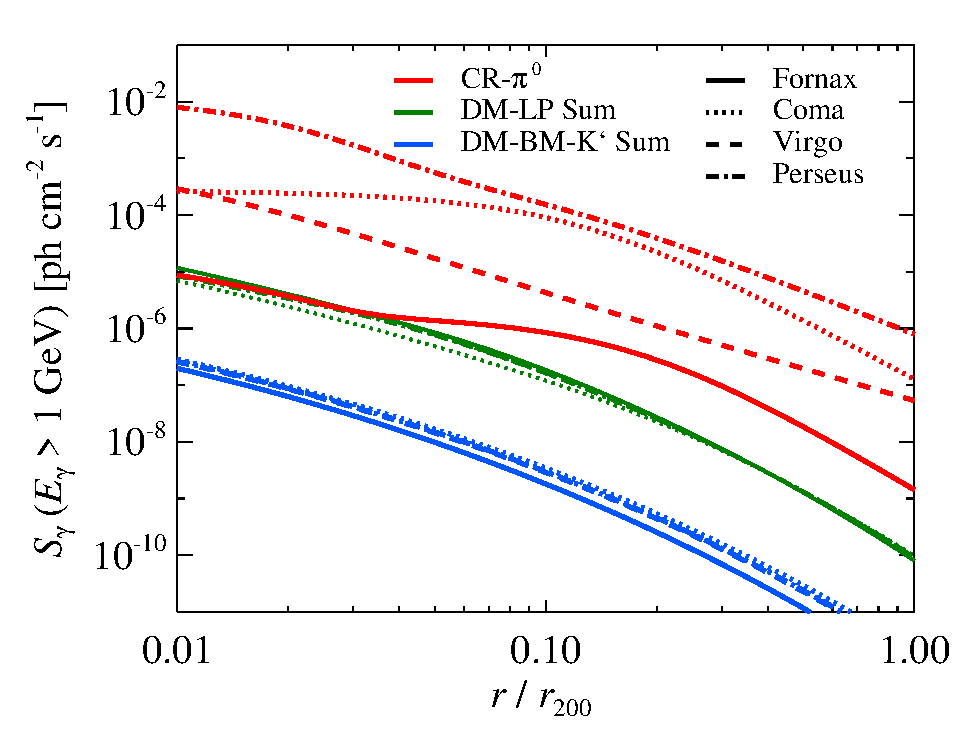
\includegraphics[width=0.49\columnwidth]{figures/SB.v13.1GeV.SF700.noSuB.elmu.eps}
  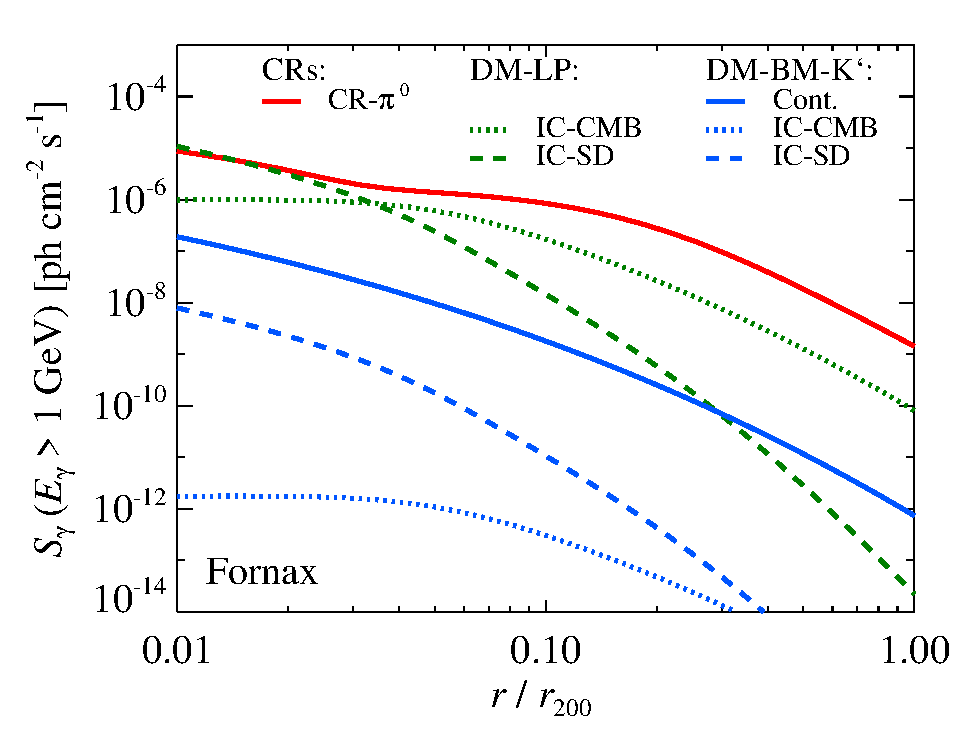
\includegraphics[width=0.49\columnwidth]{figures/SB.fornax.v13.1GeV.SF700.noSuB.elmu.eps}
  \caption{\it The intrinsic surface brightness profiles without
    substructures at energies $E>1\ GeV$. We show the CR induced
    emission (red), leptophilic emission (green), and emission from
    the $\Kp$ benchmark model (blue).  LEFT PANEL: comparison of the surface
    brightness of different clusters; Fornax (solid), Coma (dotted),
    Virgo (dashed), and Perseus (dash-dotted). RIGHT PANEL: comparison of
    different emission components in Fornax; dotted lines show the
    inverse Compton (IC) upscattered CMB photons, dashed lines show
    the IC upscattered photons from stars and dust, and blue solid
    lines show the continuum emission from the $\Kp$ benchmark model.}
 \label{fig:SB_clu_nosub}
\end{minipage}
\end{figure*}

In Sect.~\ref{sect:spectral} we saw that the spectral distribution of
gamma-ray flux from the LP model was dominated at high energies of
$E_\gamma\gtrsim 100\,$~GeV by final state radiation and IC upscattered
starlight and dust, while the BM models were mainly dominated by the
continuum emission. These high energies are observationally important
for both Fermi-LAT and Cherenkov telescopes. In
Fig.~\ref{fig:SB_IACTs}, we thus show the surface brightness above
$100\,$~GeV for a realistic PSF of $0.1\deg$ where we include the
boost from substructures. We investigate two clusters with an expected
high DM signal; the Fornax and Virgo cluster. Both clusters show a
very flat brightness profile $r<0.1\rvir$, due to both the effect from
substructures and the smoothing over the PSF. The CR induced emission
also show a smoothing in the central parts due to the PSF. In the
outer part of the Fornax cluster the CR flux is suppressed compared to
the DM flux boosted by substructures, where the LP model gives rise to
a gamma-ray flux that is more than three orders of magnitude
larger. However, it should be noted that there are large uncertainties
in the gas density profile which we use to estimate the CR induced
gamma-ray surface brightness (see Fig.~\ref{fig:dens_fornax} for more
details).

\begin{figure*}
\begin{minipage}{2.0\columnwidth}
  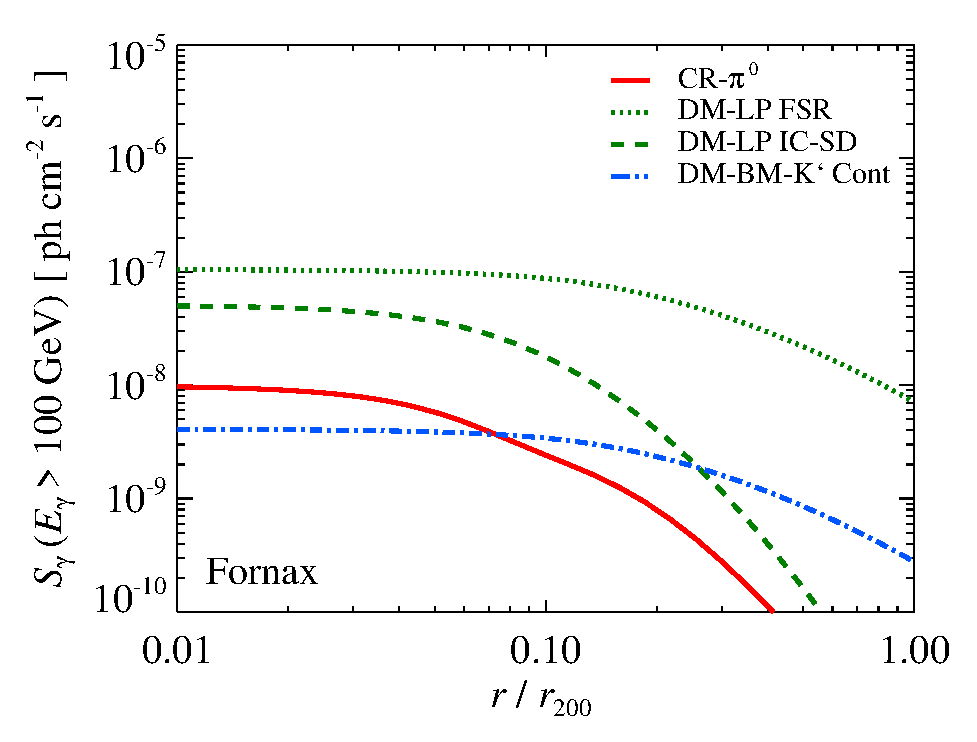
\includegraphics[width=0.49\columnwidth]{figures/SB.Fornax.v13.SF700.SubMass.elmu.eps}
  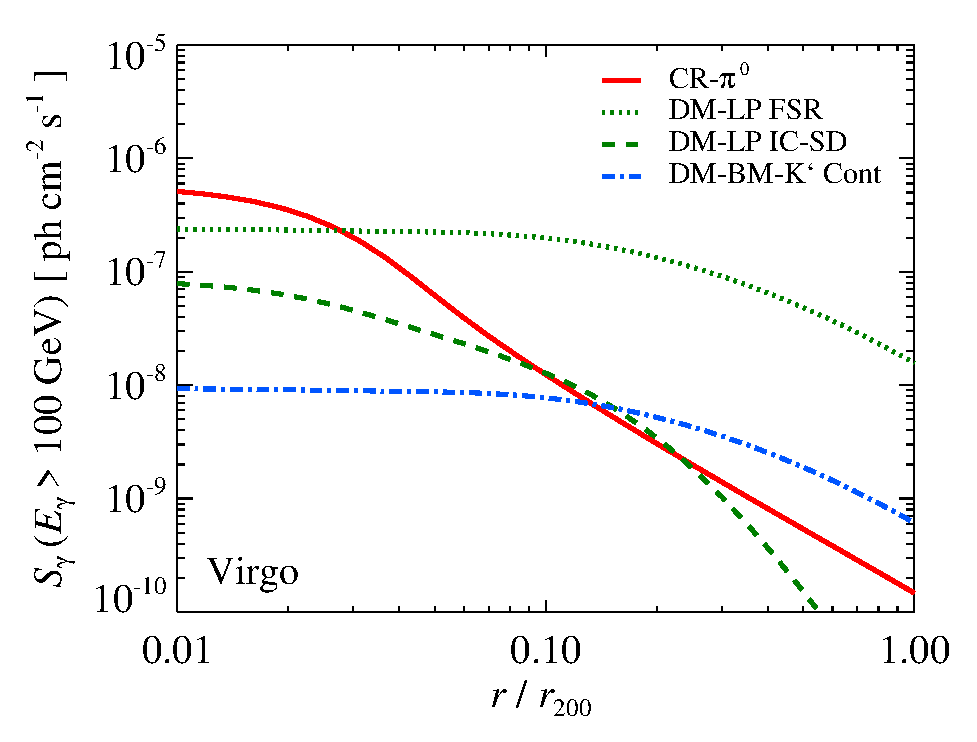
\includegraphics[width=0.49\columnwidth]{figures/SB.Virgo.v13.SF700.SubMass.elmu.eps}
\caption{\it Surface brightness predicted for Cherenkov telescopes at
  high energies. We show the emission above $100$~GeV and include the
  boost from substructures. We use a point spread function of
  $\psf=0.1\deg$ that is typical for Cherenkov
  telescopes as well as the Fermi-LAT at this energy. Left panel shows
  the Fornax cluster and right panel the Virgo cluster. The gamma-ray
  emission is derived for the following components; CRs (red solid),
  continuum emission from the DM $\Kp$ benchmark model (blue
  dash-dotted), as well as final state radiation (green dashed) and
  inverse Compton upscattered dust and starlight (green dotted) from
  leptophilic DM.}
 \label{fig:SB_IACTs}
\end{minipage}
\end{figure*}



\section{Population studies: flux predictions and observational limits}

In this section, we compute the expected gamma-ray fluxes from DM
annihilation and CR interactions of the brightest clusters of the
X-ray flux-complete sample in the local universe. We confront these
predictions to upper limits obtained by Fermi 1.5-year data and
conclude on the viability of the underlying models and perspectives
for the next years of Fermi observations.

\subsection{Scaling relations}
First we focus on gamma-ray flux-cluster mass scaling relations for DM
annihilation and CR induced emission in
Fig.~\ref{fig:lum_mass_scaling}.  
\begin{figure*}
  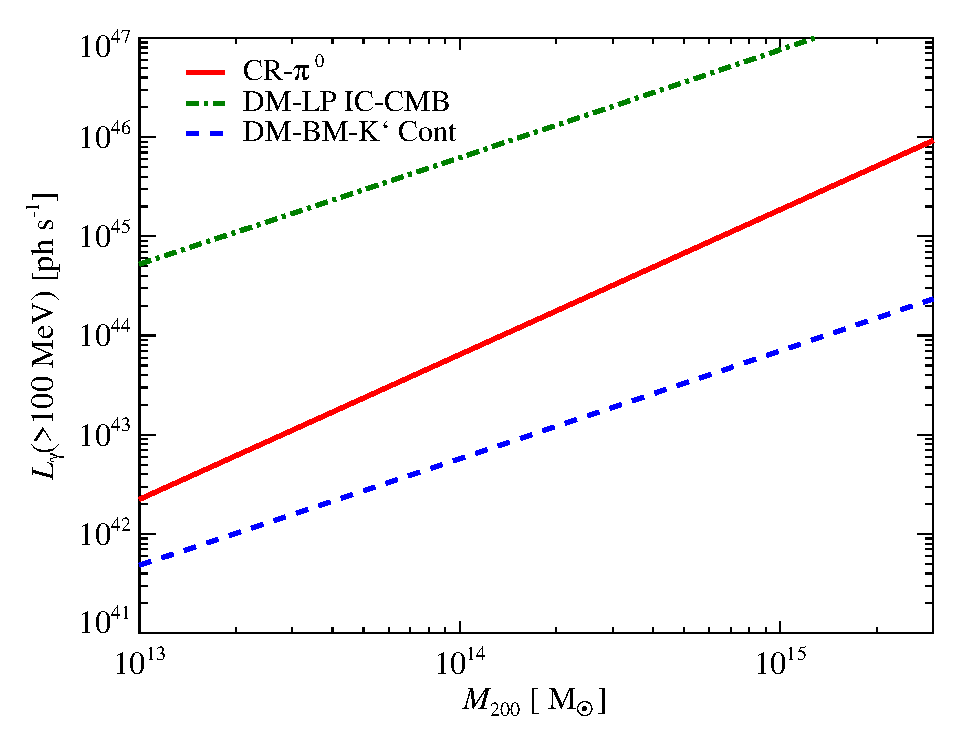
\includegraphics[width=0.99\columnwidth]{figures/MLscaling.100M.eps}
  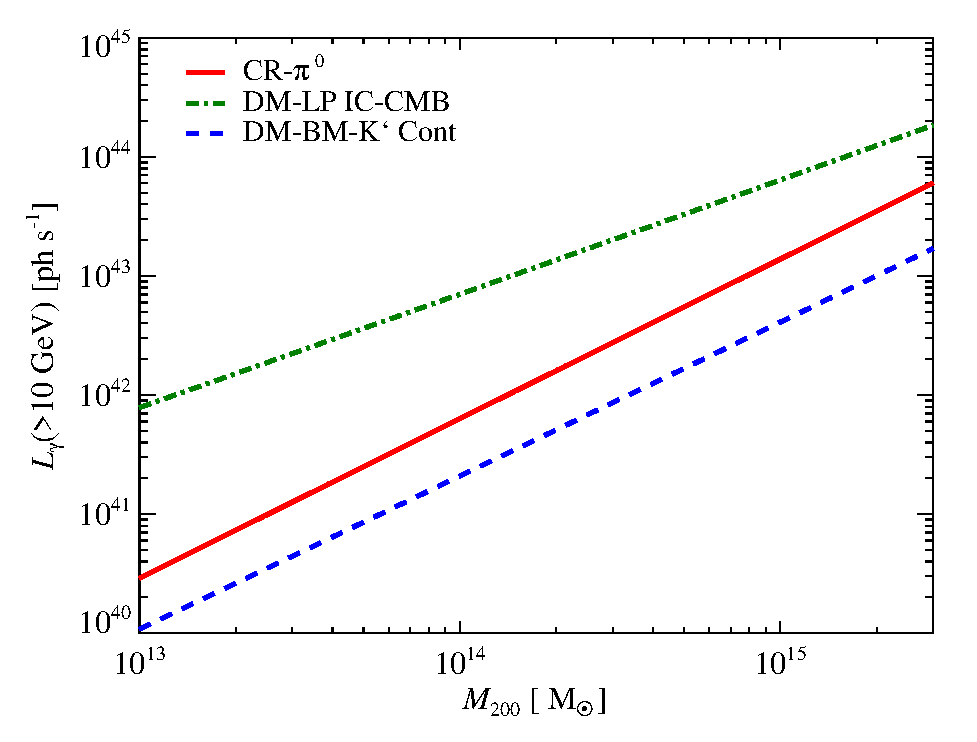
\includegraphics[width=0.99\columnwidth]{figures/MLscaling.10G.eps}
  \caption{\it Scaling relations of the cluster's virial mass $\mvir$
    and the gamma-ray luminosity for energies $E_\gamma>100$~MeV
    (left) and $E_\gamma>10$~GeV (right).  Shown are the relations for
    the CR-induced emission that is dominated by pion decay resulting
    from hadronic CR interactions (solid), the leptophilic model of DM
    annihilations \C{(dash-dotted) as well as the benchmark model $K'$
      of DM annihilation. Both DM models include the scaling of the
      substructure boost with cluster mass of
      Eq.~(\ref{eq:DM_scaling}) (dashed). Note that the scaling of the
      DM models are indicative for all (non-Sommerfeld enhanced)
      DM annihilation models while the normalization depends on the
      particular cross section and neutralino mass.}}
\label{fig:lum_mass_scaling}
\end{figure*}
\C{The mass scaling of the substructure boost steepens the
  intrinsically shallower DM annihilation relation in
  Eq.~(\ref{eq:DM_scaling}) to $L_\gamma\propto \mvir^{1.06}$.
  However, the CR scaling relation is still considerably steeper as
  shown by reference} \cite{2010MNRAS.409..449P}:
\begin{eqnarray}
L_{\gamma}(>100\,\mev) = 1.8\times10^{45}
\left(\frac{\mvir}{10^{15}\,\msun}\right)^{1.46}\mbox{erg~s}^{-1}\nonumber\\
L_{\gamma}(>10\,\gev)  = 1.4\times10^{43}
\left(\frac{\mvir}{10^{15}\,\msun}\right)^{1.34}\mbox{erg~s}^{-1}\,.\nonumber\\
\end{eqnarray}
Note that the CR luminosity scaling relations\footnote{The scaling
  relations show the flux inside $\rvir$ and do not include the
  contribution from galaxies. Also note that in this paper the scaling
  relations are normalized with $10^{15}/h_{70}\,\msun$. \C{In
    contrast, is the corresponding scaling relations in Table 5 in
    \cite{2010MNRAS.409..449P} normalized with $10^{15}/h\,\msun$
    instead of the mentioned $10^{15}/h_{70}\,\msun$. However, all
    figures/tables/equations including the scaling relation figures
    are derived for masses in units of $10^{15}/h_{70}\,\msun$.}}
include the IC gamma-ray contribution from shock-accelerated electrons
as well as secondary electrons created in CR-proton interactions. The
gamma-ray flux from the electrons is, however, dominated by the
decaying neutral pions and only show up as a small flattening of the
scaling relation at energies around $10-100\,\gev$. The steeper mass
scaling of CR emission compared to DM annihilation already implies a
general strategy to minimize the CR-induced foreground for DM
annihilation and argues for very nearby groups. We note that these
simulations do not include AGN feedback that is thought to furthermore
reduce the baryon fraction in groups relative to that in clusters
\cite{2008ApJ...687L..53P}. The resulting smaller target density for
hadronic CR interactions will furthermore steepen the $L_\gamma-M$
relation of CR induced emission, making the case for groups even
stronger.

\subsection{DM annihilation}

\begin{figure*}
\begin{minipage}{2.0\columnwidth}
  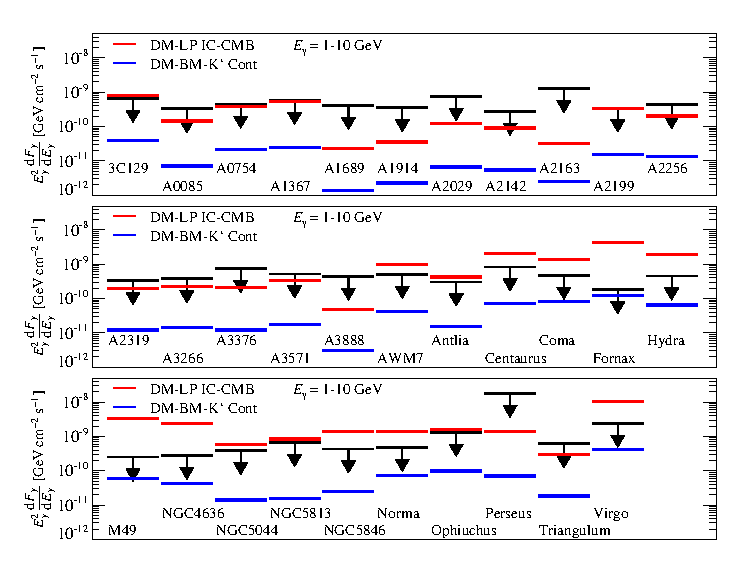
\includegraphics[width=0.99\columnwidth]{figures/Fermi.comp.DM.eps}
  \caption{\it Fermi gamma-ray flux upper limits are contrasted to the
    predicted DM gamma-ray flux. We show the mean differential flux in
    the energy range $E_\gamma=1-10$~GeV for 32 clusters. The
    \C{maximal extended Fermi-LAT upper limits are shown with black
      arrows, while the point source limits are shown in grey.} The
    predicted fluxes are derived from the dominant inverse
    Compton-scattering of CMB photons in a leptophilic DM model (red),
    and the continuum emission from the DM $\Kp$ benchmark model
    (blue). Assuming a boost factor due to substructures that has a
    mass spectrum extending down to an Earth mass, the expected
    leptophilic fluxes are ruled out by upper limits in 26 of the
    clusters, with the strongest constraints set by Fornax and
    Ophiuchus. We can not yet constrain the benchmark models,
    although improved modelling of extended sources as well as
    stacking of clusters will allow to test these in the upcoming
    years with better data.}
 \label{fig14}
\end{minipage}
\end{figure*}

\begin{figure*}%[t]
\begin{minipage}{2.0\columnwidth}
 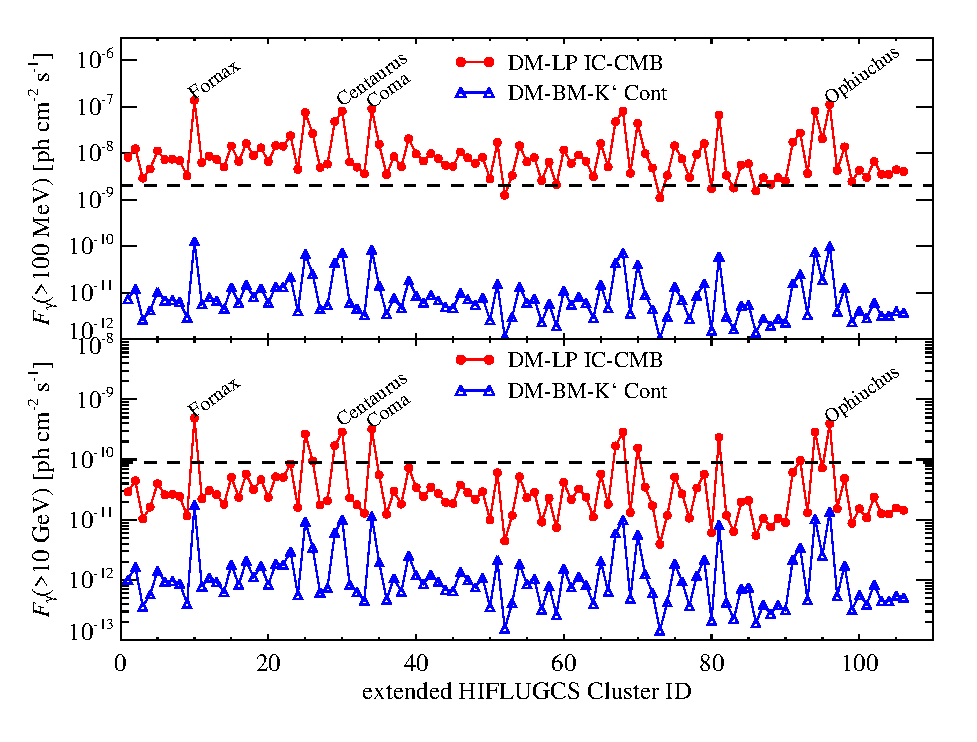
\includegraphics[width=0.99\columnwidth]{figures/Flux.comp.DM.eps}
 \caption{\it Comparing the DM annihilation flux from clusters in the
   extended HIFLUGCS catalogue. We show the energy integrated
   gamma-ray fluxes derived from both leptophilic DM that result in
   inverse Compton upscattered CMB photons (red), and the continuum
   emission from the DM $\Kp$ benchmark model (blue). The fluxes are
   calculated within $\rvir$ for each of the 106 clusters included in
   the extended HIFLUGCS catalogue. The CR emission is derived using a
   single beta profile for each cluster's gas density profile (see
   text for details). The upper panel shows the energy integrated flux
   above 100~MeV and the lower panel that above 10~GeV, both as a
   function of HIFLUGCS cluster ID. For comparison we show the
   estimated point source sensitivity of the Fermi-LAT after two years
   of data taking $F_\gamma(>100\,\rmn{MeV})\sim
   2\times10^{-9}\,\rmn{ph}\, \rmn{cm}^{-2}\,\rmn{s}^{-1}$ and
   $F_\gamma(>10\,\rmn{GeV})\sim 9\times10^{-11}\,\rmn{ph}\,
   \rmn{cm}^{-2}\,\rmn{s}^{-1}$ (dashed lines). The four brightest
   clusters are labelled yielding Fornax and Ophiuchus as the
   brightest targets.}
 \label{fig21}
\end{minipage}
\end{figure*}

Figure~\ref{fig14} compares Fermi upper limits on the gamma-ray flux
with predictions of DM annihilation fluxes in the LP and BM models.
To obtain the gamma-ray fluxes, we scale the virial mass of clusters
in the extended HIFLUGCS catalogue \cite{2002ApJ...567..716R} with our
scaling relation of Eq.~(\ref{eq:DM_scaling}). In those, we assume a
boost factor due to substructures that has a constant contribution per
decade in substructure mass and has a mass spectrum extending down to
Earth masses for our LP and BM DM annihilation models. In the LP
models we additionally assume a cluster-mass dependent boost due to
SFE. Fermi limits rule out the LP models in their present form with
the mentioned assumptions in 26 clusters, and limit the boost from SFE
to less than 14 in M49. Assuming universality, this limits the
Sommerfeld boost in the MW to less than 8 (see
Fig.~\ref{fig:boost_const}).  The flux level of the Fermi limits are
an indirect measure of the ambient background flux in the gamma-ray
sky and/or the presence of strong point sources such as AGN in the
immediate vicinity of the cluster position. Hence, the ratio of the
Fermi upper limits to the predicted annihilation fluxes,
$F_{\mathrm{UL}}/F_{\mathrm{DM}}$, is a good indication of the best
cluster candidates for indirect DM experiments. We identify Fornax,
M49, Norma, Coma, and Virgo to be prime candidates. Note however, that
Virgo extends of 12 degree over the sky which implies a lower surface
brightness and lower signal-to-noise.  Fermi limits on individual
clusters are expected to improve as $\sqrt{T/1.5 \mathrm{yr}}$, where
$T$ is the total elapsed time of the Fermi mission. We emphasize that
the very inhomogeneous distribution of $F_{\mathrm{UL}}/
F_{\mathrm{DM}}$ makes it unlikely to dramatically improve the limits
through a stacking analysis as the weak signal will dilute the average
constraints.

In Figure~\ref{fig21}, we show the DM annihilation flux predictions of
the entire sample.  Assuming the projected point source sensitivity
($5\sigma$, 50h) of the future Cherenkov telescope array (CTA) of
$F_\gamma(>E_\gamma) = \{4\times10^{-11}, 2\times10^{-12},
2\times10^{-14}\}\,\rmn{ph}\,\rmn{cm}^{-2}\,\rmn{s}^{-1}$ at energies
of $E_\gamma=\{10~\rmn{GeV}, 100~\rmn{GeV}, 1~\rmn{TeV}\}$
\cite{Doro:2009qs}, we note that it will be very challenging to detect
the DM annihilation signal from clusters without a Sommerfeld boost by
Cherenkov telescopes.  This is because the boost from substructures is
extended while the sensitivity of Cherenkov telescopes scales
\C{approximately linearly with source extension}. Hence the fluxes
quoted in Fig.~\ref{fig21} will have to be compared to a sensitivity
that is scaled down by the ratio of cluster radius to angular
resolution of 0.1 degree assuming current background subtraction
techniques of Cherenkov telescopes. This important finding should
encourage the development of new methods to overcome the degradation
of sensitivity for diffuse and very extended sources. Such a
break-through would be needed to probe and potentially detect the
presented class of BM models with a large investment of observational
time.


\subsection{CR-induced emission}
\label{sec:CRemission} 
\begin{figure*}
\begin{minipage}{2.0\columnwidth}
  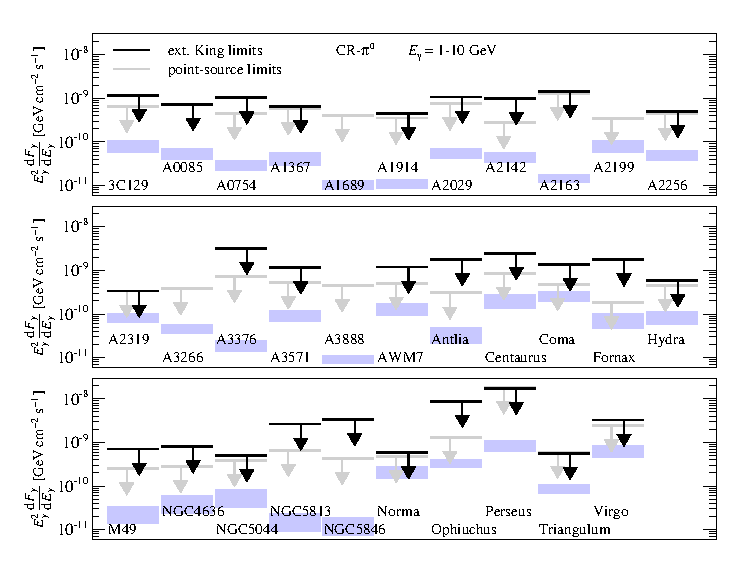
\includegraphics[width=0.99\columnwidth]{figures/Fermi.comp.CR.diff.eps}
  \caption{\it We contrast predictions of the CR induced gamma-ray
    emission using an analytical CR model \protect
    \cite{2010MNRAS.409..449P} to Fermi-LAT flux upper limits. We show
    the mean differential flux in the energy range $E_\gamma=1-10$~GeV
    for 32 clusters. \C{The extended Fermi upper limits assume King
      profiles and are shown with black arrows, while the point source
      limits are show with grey arrows.} The blue boxes show the
    gamma-ray emission from CR-induced $\pi^0$-decay, where the upper
    (lower) bounds show the estimates for an optimistic (conservative)
    model (see Sect.~\ref{sec:CRemission} and
    \cite{2010MNRAS.409..449P} for details). Note that our models are
    in perfect agreement with the derived upper limits from
    Fermi. Interestingly, the limits of Virgo, Norma, and Coma are
    closing in on our predictions and will enforce constraints on the
    parameters of hadronic models such as shock acceleration
    efficiencies or CR transport properties in the coming years.}
 \label{fig15}
\end{minipage}
\end{figure*}

\C{In Fig.~\ref{fig15}, we show the extended Fermi-LAT flux upper
  limits that assume King profiles that trace the X-ray emitting gas
  compared to the flux predictions by an analytical CR model
  \cite{2010MNRAS.409..449P} for CR induced gamma-rays.} For
consistency, we use beta-model fits to ROSAT data of X-ray bright
clusters for our gamma-ray flux estimates as an input
\cite{2002ApJ...567..716R}). We derive the central gas densities for
each cluster by following the approach outlined in
\cite{1999ApJ...517..627M} which assumes that the ICM is
isothermal. The central gas density is found by combining X-ray
temperature with X-ray luminosity, X-ray detection radius, density
core radius and density slope for each cluster. These predictions are
superior to those that use luminosity-mass scaling relation to infer
the expected gamma-ray flux---a method used by reference
\cite{2010ApJ...717L..71A} to compare to Fermi limits.  In this
analytic model, we employ the fact that CRs accelerated at structure
formation shocks and transported over cosmic time. This leads to a CR
distribution with a universal spectral form and an almost universal
spatial distribution. Depending on whether or not we account for the
bias of ``artificial galaxies'' in cosmological simulations, we derive
an optimistic or conservative limit of the expected gamma-ray emission
from decaying pions (bracketing our ignorance of the contribution of
cluster galaxies to the overall gamma-ray flux from a cluster). Note
that both models assume the maximally allowed acceleration efficiency
for strong shocks that transfers 50\% of the shock-dissipated energy
(kinetic energy corrected for adiabatic compressional heating at the
shock) to CRs. These efficiencies drop quickly for weaker shocks
\cite{2007A&A...473...41E} which dominate the gravitational energy
dissipation inside galaxy clusters \cite{2006MNRAS.367..113P}. These
efficiencies will have to be corrected down if this value is not
realized at structure formation shocks. Secondly, these simulations
neglect active CR transport such as streaming and diffusion relative
to the gas, i.e. we assume that advective transport is the dominant
one and CRs are tightly coupled to the gas via flux-frozen magnetic
fields tangled on sufficiently small scales. Evidence from the
statistics of radio halos suggests that this might not be the case for
relaxed clusters, arguing that CR streaming in those objects could be
responsible for a decrease in the central CR number density. This
effect would also reduce the expected gamma-ray flux by up to a factor
of five \cite{2011A&A...527A..99E}. We note that the tightest Fermi
limits are obtained in the 1-10 GeV regime due to the highest
sensitivity of Fermi-LAT there. While the effective area of LAT
increases up to these energies, the typical photon spectra decrease as
a function of energy: combining those effects selects this energy
range to be most sensitive.  In this energy band, the Fermi limits
come close to the flux predictions of Virgo, Coma and Norma. Using
integrated flux limits from Fermi, we arrive at very similar results.
We emphasize that by using our analytic modeling, the slight
discrepancy of the scaling relation-based prediction with the Fermi
limit on Norma \cite{2010ApJ...717L..71A} is resolved: Norma simply
seems to be less bright than an average cluster of the same mass as
Norma. The insensitive limit on Perseus \C{is due to the bright
  central source NGC1275 with an AGN in the center
  \cite{2010ATel.2916....1M} making it hard to determine a comparable
  limit as obtained for the other clusters. In addition, there are
  recent gamma-ray observations of the head-tail radio galaxy IC310 in
  the cluster outskirts
  \cite{2010ApJ...723L.207A,2010A&A...519L...6N}.}

\C{A quantity that is of great scientific interest is the CR pressure
  ($P_\CR$) relative to the thermal pressure ($P_\rmn{th}$) as it
  directly bias galaxy cluster observables and the resulting
  cosmological constraints, such as the hydrostatic mass bias or the
  Sunyaev-Zel’dovich signal measured by Planck, South Pole Telescope,
  or Atacama Cosmology Telescope. In the following we estimate the
  mass scaling of the relative CR pressure, $X_\CR =
  P_\CR/P_\rmn{th}$, using the CR formalism outlined in
  \cite{2007A&A...473...41E,2010MNRAS.409..449P}. We derive the CR
  pressure from the CR distribution function $f = C\,p^{-\alpha}$,
  where $C$ is the normalization of each power-law, $p=P/m_\rmn{p} c$
  is the normalized CR proton momentum, and $\alpha$ is the CR
  spectral index. The pressure is given by $P_\CR \propto
  C=\tilde{C} \,\rho_\rmn{gas}$, where $\tilde{C}\propto M^{0.44}$ for
  clusters with a mass $\mvir\gtrsim 10^{14}\,\msun$
  \cite{2010MNRAS.409..449P}. We determine the mass scaling of the gas
  density through its relation to the enclosed gas fraction
  $f_\rmn{gas}$, and find that $\rho_\rmn{gas}\propto f_\rmn{gas}
  \propto M^{0.135}$ \cite{2009ApJ...693.1142S}. The thermal pressure
  is derived from the temperature in virial equilibrium, and scales as
  $P_\rmn{th}\propto k_\B T \propto G M/R \propto M^{0.67}$. Finally
  we can derive the mass scaling of the volume weighted relative CR
  pressure from
\begin{equation}
 <X_\CR> = \frac{<P_\CR>}{<P_\rmn{th}>} \propto \frac{<\rho_\rmn{gas}\,
   \tilde{C}>}{<k_\B T>} \propto M^{-0.1}\,,
\end{equation}
which is roughly a constant, i.e. almost independent on halo
mass. This suggests that CRs are acclerated at the strongest shocks,
in the early universe or between voids and pre-collapsed IGM, and then
experience a similar transport history in the form of adiabatic
compression or similarily weaker shocks. Since the CRs that build up
the bulk of the CR pressure also give rise to gamma-ray emission
through the production of decaying pions, we use gamma-ray upper
limits from Fermi-LAT to constrain $X_\CR$. In Fig.~\ref{fig:XCR} we
show the volume weighted relative CR pressure for 32 clusters, for
which LAT upper limits that assume King profiles are derived. We adopt
a constant $<X_\CR>\approx 0.02$ derived from a representative
simulated cluster \cite{2008MNRAS.385.1211P} and find that for most of
the clusters in the sample we can constrain $X_\CR < (0.1-0.2)$ using
the extended gamma-ray upper limits, where the most constraining
clusters are Norma and Coma with $X_\CR < 0.07$. Most of the 32
clusters have $X_\CR$ upper limits within a factor few from the best
constraining clusters, which suggests that stacking of clusters will
be able to improve these limits. This might even be improved further
using a scaled stacking with our model as a prior. In a recent work
\cite{2010ApJ...717L..71A}, where the 1.5 year Fermi data was used to
derive limits on $X_\CR$, they found that the most massive clusters
are on average more constraining, while we find better limits on the
low mass clusters. This difference is explained by the different
priors on $P_\CR$; they assumed a mass independent CR pressure derived
from a single CR power-law distribution function, while we adopt a
prior inferred from cosmological simulations that dynamically trace the
CRs during cluster assembly and allow for a varying spectral index
where $P_\CR\sim M^{0.44}$. Furthermore, the gamma-ray flux
predictions that we use in this work to constrain $X_\CR$ assumes the
true gas density distribution for each cluster \footnote{Derived from
  the parameters in the extended HIFLUGCS catalogue.} that accounts
for cluster-to-cluster scatter, in contrast to the mass-to-luminosity
scaling relations that was used in previous work.}

\begin{figure*}
\begin{minipage}{2.0\columnwidth}
  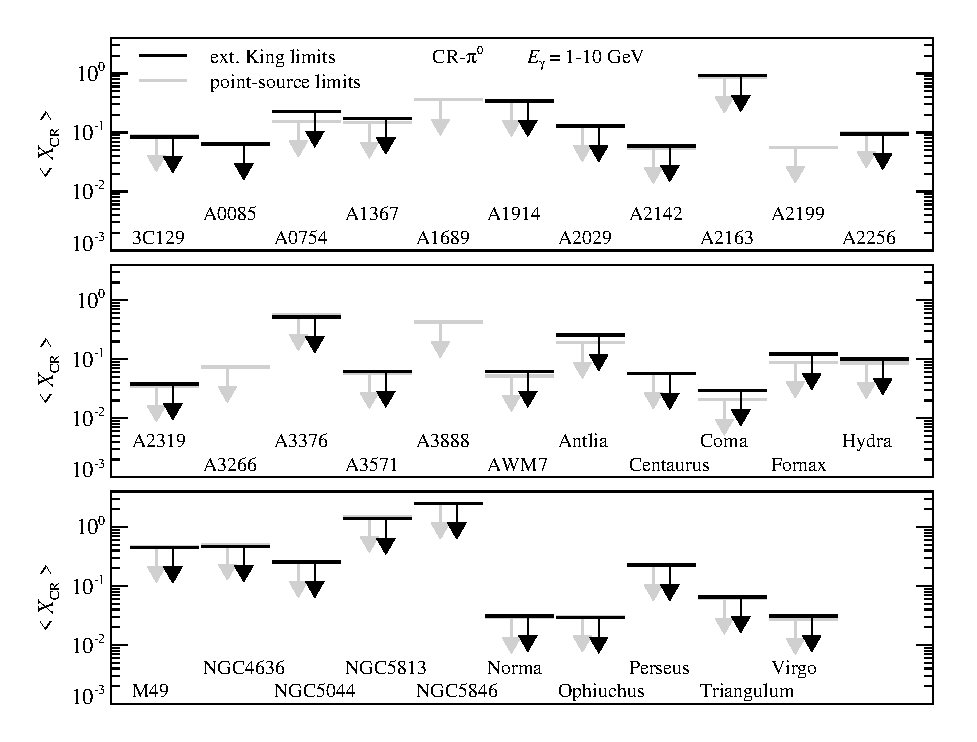
\includegraphics[width=0.99\columnwidth]{figures/XCR.Fermi.eps}
  \caption{\it Limits on the relative CR pressure, $< X_\rmn{CR}> = <
    P_\rmn{CR} > / < P_\rmn{th}>$ averaged across the cluster. Our
    constraints are obtained with the extended Fermi-LAT limits in the energy
    range $E_\gamma=1-10$~GeV that assume a King profile which matches the
    extension of the thermal X-ray emission (black) and for comparison with
    Fermi-LAT point-source limits (grey) \cite{2010ApJ...717L..71A}. In
    computing those limits, we adopted our (conservative) analytic model
    \cite{2010MNRAS.409..449P} and an averaged relative CR flux as obtained from
    our simulations.}
 \label{fig:XCR}
\end{minipage}
\end{figure*}

To complete this section, we present our analytical model predictions
for the CR-induced gamma-ray flux for all clusters in the extended
HIFLUGCS sample in Fig.~\ref{fig19}. In the lower panel of this
figure, we show the relative difference between the gamma-ray flux
computed using the analytical CR model to the flux predicted by the
mass-luminosity scaling relation. Statistically, one can view the
analytical modeling as explicitly accounting for the scatter of the expected
gamma-ray flux at a given mass. Cool core clusters have a denser core
which increases the target density of gas protons for the hadronic
reaction which in turn leads to a systematic increase of the expected
gamma-ray fluxes. We confirm this effect since all clusters with
increased flux ratio of our analytical CR model relative to the scaling relation
expectation are in fact cool core clusters. This suggests that the X-ray
emission should be a good proxy for the expected gamma-ray
emission. Note however that there could be the counter-acting effect
of CR streaming in relaxed clusters which would tend to decrease the
gamma-ray luminosity \cite{2011A&A...527A..99E}. Future careful
modelling is needed to quantify this effect.

\begin{figure*}%[t]
\begin{minipage}{2.0\columnwidth}
 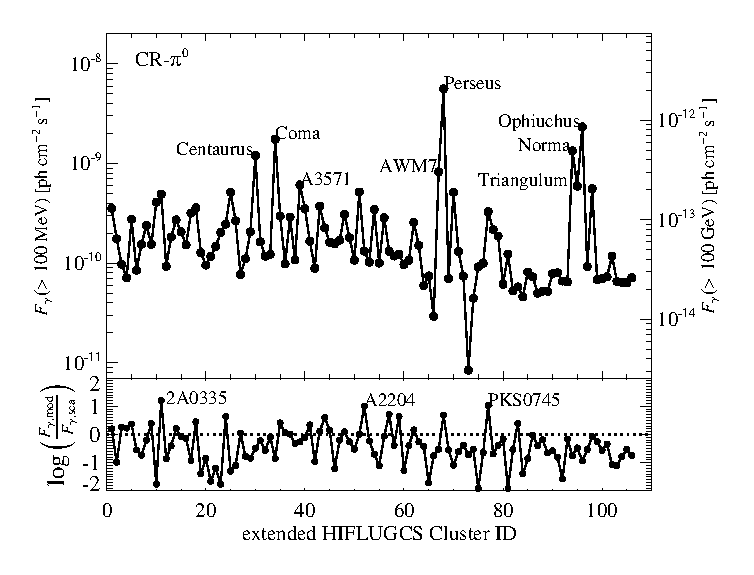
\includegraphics[width=0.99\columnwidth]{figures/Flux.comp.CR.eps}
 \caption{\it Comparison of the gamma-ray flux induced by CRs for the
   106 clusters included in the extended HIFLUGCS catalogue.  The CR
   distribution follows the analytical model derived through
   hydrodynamical cosmological cluster simulations \protect
   \cite{2010MNRAS.409..449P} (see text for details).  Gamma-ray
   fluxes are calculated within $\rvir$ and are derived using a single
   beta profile for each cluster's gas density profile as obtained by
   ROSAT X-ray observations. The upper panel shows the energy
   integrated flux above 100~MeV (left side) and above 100~GeV (right
   side), both as a function of HIFLUGCS cluster ID. The eight
   brightest clusters are labelled. The lower panel shows the relative
   difference between the the flux computed using the analytical model
   and the gamma-ray flux predicted by the mass-luminosity scaling
   relation \cite{2010MNRAS.409..449P}. The clusters with the largest
   positive offset are labelled. As expected, they all are cool core
   clusters.}
 \label{fig19}
\end{minipage}
\end{figure*}


\section{Conclusions}

In this paper, we study the possibility for detecting gamma-ray
emission in galaxy clusters. We consider benchmark (BM) and
leptophilic (LP) models of supersymmetric dark matter (DM) as well as
cosmic ray (CR) induced pion decay which is thought to dominate the
astrophysical signal from clusters. Once supersymmetric cold dark
matter decouples from the expanding universe it streams and erases any
potentially present smaller scales. When gravitational instabilities
causes halos to collapse, this free-streaming scale imprints as a
characteristic minimum halo mass $M_\mathrm{min}$ into the hierarchy
of structure formation and should still survive until the present time
as substructure within larger halos. It turns out that the boost due
to substructures dominates over the smooth component for halo masses
$\mvir>10^3 \msun$ and contributes a constant luminosity for each
decade in halo mass. The ratio of halo-to-minimum subhalo mass
$\mvir/M_\mathrm{min}$ is maximized for the largest systems that had
time to collapse and virialise since the Big Bang -- galaxy
clusters. The corresponding substructure boost can reach values
exceeding $10^3$ which should make nearby clusters the brightest DM
annihilation sources after the MW center and hypothetical very
close-by DM substructures.  Since the mass density of substructures
peaks at radii close to $\rvir$, the contribution to the annihilation
emission from substructures is also dominated from these outer cluster
regions.  This implies an almost flat surface brightness profile of
the annihilation emission which makes it necessary to have the entire
cluster in the field-of-view to take advantage of the total
substructure boost. This property makes it difficult to detect DM
annihilation emission without an enhancement of the particle physics
cross section over its standard value of $\sigma v\sim 3\times
10^{-26} ~\mathrm{cm}^3~\mathrm{s}^{-1}$ with imaging air Cherenkov
telescopes due to the spatially extended boost from substructures of
angular extent $\sim 0.5-1\deg$ (as independently found by reference
\cite{2011arXiv1104.3530S}). In contrast, the sensitivity of Cherenkov
telescopes drops linearly with radius outside the point spread
function $\sim 0.1\deg$, unless new background subtraction schemes can
be found, e.g., for the survey mode of CTA.

We identify Fornax to be the best cluster/group candidate for indirect
DM studies as it is expected to emit the brightest annihilation flux
and more importantly, has a comparably low CR induced gamma-ray flux.
\del{This in principle should allow to detect or constrain some BM
  models that have been chosen for the large gamma-ray flux yield with
  three-year Fermi data (or constrain the substructure boost factor).}
Other nearby bright sources of the extended HIFLUGCS sample of nearby
bright X-ray cluster/groups are M49, Centaurus, and NGC~4636.  The
non-detection of gamma-ray emission by Fermi in a total of 26
clusters/groups (the mentioned clusters as well as Virgo, Coma, Hydra,
and Norma among others) considerably constrains LP models for DM
annihilation which were introduced to explain the increasing
positron-to-lepton ratio beyond 10 GeV. \C{Assuming that the minimum
  DM substructure mass extends down to an Earth mass, we limit the
  saturated Sommerfeld enhancement factor in M49 and Fornax to about
  14 and 22, respectively. This corresponds to a value in the Milky
  Way (MW) of less than 8 and 13 due to the larger Sommerfeld boost
  factor in smaller mass halos which have a lower velocity dispersion
  that enhances the particle cross section (while assuming
  universality of the DM model).} This would rule out LP models in
  their current form based on the non-observation of gamma-rays in any
  of the fore-mentioned clusters/groups. Alternatively, assuming the
  LP models to be correct, we limit the minimum substructure mass to
  $>10~\msun$ in M49.

In this work, we thoroughly study the spectral emission
characteristics of the DM emission. In general there are different
radiation mechanism that emit in the gamma-ray regime, namely (i)
continuum emission following the hadronization of the annihilating
neutralinos in BM models which leads to the production of charged and
neutral mesons which decay finally into electrons, neutrinos, and
gammas, (ii) inverse Compton (IC) emission by the leptons in the final
state which up-scatter radiation fields from the cosmic microwave
background (CMB), dust, and starlight, and (iii) final state radiation
or internal bremsstrahlung which dominates the highest energy emission
close to the rest mass of the self-annihilating neutralinos (if
present in the model under consideration). While this final state
radiation is sometimes not distinguished from the continuum emission
contribution, we keep it separate as it dominates the very high-energy
tail of the gamma-ray spectrum in LP models while there the continuum
emission is negligibly low.

For the first time, we compute the IC emission component not only from
the upscattered CMB photons but also from a realistically modeled
photon field due to dust and starlight extending from infra-red to
optical wavelengths. To this end, we construct a rather simple
analytic model for the spatial and spectral distribution of dust and
starlight in clusters which can be used for the annihilation emission
in galaxies with a different spatial profile.  We find that in BM
models, the continuum emission dominates over the IC emission of any
available radiation field. In the LP models, where the continuum
emission is low, the IC up-scattering of the CMB dominates below 60
GeV. \C{The final state radiation then takes over for energies up to
  the cutoff at $m_\chi c^2 \sim 1$~TeV. The IC up-scattering of the
  dust and starlight is always subdominant compared to the upscattered
  CMB (below 60~GeV) and the final state radiation (above 60~GeV).}
\del{For large clusters, the final state radiation then takes over for
  energies up to the cutoff at $m_\chi c^2 \sim 1$~TeV. In small
  clusters, there is a window around $E_\gamma \sim 100~\mathrm{GeV}$
  where the IC up-scattering of the dust emission dominates over the
  CMB IC emission and the final state radiation. The IC emission of
  starlight remains always subdominant.}  We stress, that the
inclusion of the dust and starlight radiation fields are negligible in
the cooling function for the leptons.  The main reason why the IC
emission from starlight and dust remains subdominant is the small
overlap of this component with the peripherally peaked substructure
mass density profiles. If for some reason, DM has less substructure,
the relative importance of this IC component increases considerably.

We substantially improve the modelling of the expected gamma-ray
signal from pion-decay resulting from hadronic CR interactions with
gas protons over previous work \citep{2010ApJ...717L..71A}. We employ
the analytic model of the CR spectrum and spatial distribution,
recently developed by \citet{2010MNRAS.409..449P} that is based on
cosmological hydrodynamical simulations of galaxy clusters that
self-consistently follow the evolution of CRs in cosmic structure
formation. Adopting the model for all clusters in the HIFLUGCS sample
of flux-limited X-ray clusters, we compare the expected gamma-ray
emission to that inferred from using $L_\gamma$-cluster mass scaling
relation. We note that the predictions of our ``optimistic'' model are
perfectly in agreement with Fermi upper limits for all clusters.  The
hint of a tension that the scaling relation modeling showed for Norma
\citep{2010ApJ...717L..71A} could not be confirmed due to the lower
gas density of this cluster relative to the average.  As expected, the
analytical CR model accounts for the ``scatter'' to the scaling
relation and biases the gamma-ray flux high for prominent cool core
clusters by up to a factor of 6 relative to the expectation from the
scaling relation. This is due to the high target gas densities and
associated CR densities in those cool cores that shape the spatial
emission characteristic to be very similar to that observed in thermal
X-rays. We caution that these predictions only apply for the case of
negligible active CR transport such as CR streaming and diffusion
relative to the gas. Gamma-ray fluxes might be considerably smaller in
those cluster that do not show an extended diffuse radio(-mini) halo
that might point to a centrally concentrated CR distribution
\citep{2011A&A...527A..99E}. The CR spectrum $E^2 dN/dE$ shows the
characteristic pion bump at energies around 1~GeV. It is expected to
dominate the DM annihilation signal of BM models for all
clusters/groups but Fornax. \C{We conclude that due to the large
  spatial extension of the brightest clusters it is not possible for
  Fermi to rule out the LP model or to constrain the BM DM models
  without improved modelling. However, we can put tight constraints on
  the boost from substructures and Sommerfeld enhancement using the LP
  model. Hence, clusters are a nice complement to direct and
  accelerator searches for the nature of DM.}\del{We conclude that it
  will be possible to rule out the LP model with six years of Fermi
  data and start to constrain some BM DM models. Hence this should
  nicely complement direct and accelerator searches for the nature of
  DM.}




%------------------------------------------------------------------


\smallskip We would like to thank Volker Springel, Megan Donahue,
Stefano Profumo, Tesla Jeltema and Fabio Zandanel for helpful
discussions.  In addition we thank Neal Weiner and Tracy Slatyer for
many comments and suggestions for improvements of a previous version
of this paper. A.P. acknowledges NSF grant AST 0908480 for support. We
would furthermore like to thank KITP for their hospitality during the
galaxy cluster workshop.  This research was supported in part by the
National Science Foundation under Grant No. NSF PHY05-51164.
C.P. gratefully acknowledges financial support of the Klaus Tschira
Foundation. The work of L.B. was supported by the Swedish Research
Council (VR), under contracts no. 621-2009-3915 and 349-2007-8709 (the
Oskar Klein Centre).


%-) Consider having one figure where we compare the Einasto profile, to
%NFW, NFW w/ beta 0.6, and also the effect of a different concentration
%mass-scaling relation
%
%-) also, plot BM flux vs. psf, for models w/ and w/o substructures


%%%%%%%%%%%%%%%%%%%%%%%%%%%%%%%%%%%%%%%%%%%%%%%%%%%%%%%%%%%%%%%
\vspace{-0.7cm}
\bibliography{bibtex/paper}
%\bibliography{apssamp}
%\bibliographystyle{apsrev4-1}

\appendix

\section{Detailed modelling of starlight and dust in clusters}
\label{sect:SD}
In this section, we present the details of our model of stars and dust
(SD) in clusters of galaxies. In the first part, we use the measured
spectral distribution of light from SD in a typical galaxy to derive a
simple spectral model for SD in galaxy clusters. This is done by
renormalizing the galactic SD distribution to match the observed luminosity
from a cluster in the far infra-red (IR) and ultra-violet (UV) bands
separately. In the second part, we derive the spatial distribution of
the SD light from a stacked sample of clusters.

\subsection{Energy spectrum}
The cluster emission from far-IR to optical/UV is due to dust emission
and stellar light, respectively. We distinguish three components: the
brightest cluster galaxy (BCG), the intra-cluster light (ICL) and
individual galaxies. While the latter distribution is highly clumped,
the first two components are smoothly distributed.  We use the far-IR
to UV spectrum derived in reference \cite{2006ApJ...648L..29P} for a
Milky Way (MW)-type galaxy to characterize the spectral distribution
of SD in a cluster. Note that we only keep the spectral shape, and
renormalize the amplitude of the spectral distribution using the
luminosity from SD in clusters.

In Fig.~\ref{fig:SD_spectra}, we show the cosmic microwave background
(CMB) black-body distribution together with the spectral distribution
of SD light of a $6.0\times10^{14}\,\msun$ galaxy cluster. We fit the
spectral shape of SD individually; the dust that peaks at about
$10^{-2}\,\ev$ is fitted using a double power-law, while the broader
spectral distribution of the stars that peaks at about $1\,\ev$ is
fitted using a triple power-law. The best fit to the galactic spectrum
is given by:
\begin{eqnarray}
  u_\stars^\gal(\eph) &=& \frac{23\,\rmn{eV}}{\rmn{cm}^3} 
  \left(\frac{1.23\,\rmn{eV}}{\eph}\right)^{1.9} \nonumber \\
  &\times&\left[1+\left(\frac{2.04\,\rmn{eV}}{\eph}\right)^{20}\right]
  ^{-\frac{1.9}{20}}\nonumber \\
  &\times& \left[1+\left(\frac{0.78\,\rmn{eV}}{\eph}\right)^{20}\right]^{-\frac{2.6}{20}}\,, \\
  u_\dust^\gal(\eph) &=& 
  \frac{40\,\rmn{eV}}{\rmn{cm}^3} 
  \left(\frac{0.0144\,\rmn{eV}}{\eph}\right)^{4.9}\nonumber \\
  &\times& \left[1+\left(\frac{0.0144\,\rmn{eV}}{\eph}\right)^{1.9}\right]^{-4.9}\,.
\end{eqnarray}
The specific energy density of the light from SD in a cluster can now
be derived from
\begin{eqnarray} 
u_\sd(\eph, r) &=& j(r)\,u_\sd(\eph)\,,
\label{eq:u_SD_er}
\end{eqnarray}
where the spectral distribution of SD is given by
\begin{eqnarray}
  u_\sd(\eph) &\equiv& \eph^2\frac{\dd^2 N_\ph}{\dd \eph \dd V}
  =  \sum_i N_i(\mvir) u_i^\gal(\eph)\,,\nonumber \\ 
\rmn{for}\quad i&=&\{\rmn{stars,dust}\}\,.
\end{eqnarray}
Here $\eph$ denotes the energy of the SD photons, $j(r)$ describes the
unitless spatial distribution of SD (derived in
Sect.~\ref{sect:SD_radial}), and $N_i(\mvir)$ denotes the mass
dependent normalization for the SD. This function is determined using
the total energy of the light from SD within $\rvir$ which is
represented by $E_{i,\vir}$. We relate this energy to the luminosity
$L_i$ in each respective wavelength band (far-IR light for the
dust, and optical/UV light for the stars) using
\begin{eqnarray} 
  E_{i,\vir} &=& L_i \frac{\rvir}{c} \nonumber \\
  &=&N_i(\mvir)\int_{\rvir} \int_i \,j(r) 
  \frac{u_i^\gal(\eph)}{\eph}\,\dd V\dd \eph\,,\nonumber \\
 \rmn{for}\quad i&=&\{\rmn{stars,dust}\}\,.
\label{eq:E_SD}
\end{eqnarray}
Here we approximate the total energy of the photons within $\rvir$
with the SD luminosity multiplied with the typical timescale that it
takes for a photon to propagate through the cluster (we assume that
the cluster is optically thin).

The {\em luminosity from star light} is given by
\begin{eqnarray}
L_\stars(M_{200\rmn{av}})&=&10^{\frac{m_\odot-m_\rmn{cl}-2.5\log\left(1+z\right)}{2.5}}
\left(\frac{D_\clu}{D_\odot}\right)^2 L_\odot\nonumber\\
&\approx& 5.3\times10^{44}\,\rmn{erg}\,\rmn{s}^{-1}\,,
\label{eq:L_stars}
\end{eqnarray}
where the average apparent magnitude of a cluster at $z\approx 0.25$
in the $(r+i)$-band is given by $m_\rmn{cl}\approx 15.5$
\cite{2005MNRAS.358..949Z}. This magnitude is derived from stacked
clusters observed by the SDSS with the average mass
$M_{200\rmn{av}}=4.0\times10^{13}\msun$. We also use an apparent
magnitude of the sun $m_\odot\approx -27.7$, distance to the sun
$D_\odot=4.85\times10^{-6}\,\rmn{pc}$, luminosity of the sun
$L_\odot=1.17\times10^{33}\,\rmn{erg\,s}^{-1}$, and distance to the
cluster average of $D_\clu=1.26\times10^9\,\rmn{pc}$. Furthermore, to account for
different cluster masses, we employ a simple mass scaling for the
luminosity from  stars in Eq.~(\ref{eq:L_stars}). Here we assume
that the total starlight has the same halo mass scaling as the
brightest cluster galaxy (BCG) \cite{2010ApJ...713.1037H}, which is a
reasonable assumption since a large contribution of the smoothly distributed
starlight in a cluster comes from the BCG. The starlight luminosity as
a function of mass is given by
\begin{equation}
L_\stars(\mvir)=L_\stars(M_{200\rmn{av}})\,
\left(\frac{\mvir}{M_{200\rmn{av}}}\right)^{0.18}\,.
\label{eq:L_stars_m}
\end{equation} 
We can now fix the unitless normalization constant for the stars in
Eq.~(\ref{eq:E_SD}) by integrating over the cluster volume and
spectral distribution of the stars:
\begin{equation}
 N_\stars(\mvir) = 
\left(\frac{\mvir}{M_{200\rmn{av}}}\right)^{0.18}\,
\frac{\rvir\, 6.0\times10^{-9}\,\kpc^2}{\int_{\rvir} j(r) \,\dd V}\,.
\label{eq:N_stars}
\end{equation}

The {\em luminosity from  dust} is derived from the
luminosity-richness scaling relation found in
\cite{2008A&A...490..547G}
$L_\dust=10^{44.8}\left(\frac{N_{200}}{10}\right)^{0.8}$. We pick a
high richness cluster with $N_{200}=82$ to normalize the luminosity
since these clusters are less likely biased by chance
coincidences. This richness  corresponds to a virial mass of approximately
$M_\rmn{200dust}=6.0\times10^{14}\,\msun$
\cite{2010ApJ...713.1037H}. We assume that the dust scales with halo
mass in the same way as the stars, and determine the normalization
constant for the dust in Eq.~(\ref{eq:E_SD}) to
\begin{equation}
 N_\dust(\mvir) = 
\left(\frac{\mvir}{M_\rmn{200dust}}\right)^{0.18}\,
\frac{\rvir\,4.0\times10^{-7}\,\kpc^2}{\int_{\rvir} j(r) \,\dd V}\,.
\label{eq:N_dust}
\end{equation}


\subsection{Radial profiles}
\label{sect:SD_radial}
Our goal in this section is to derive a simple spatial model for the
distribution of the light from SD in galaxy clusters. For this reason
we use stacked cluster observations from the Sloan Digital Sky Survey
(SDSS) in the $r$ and $i$-band that trace the starlight. For
simplicity we assume that the dust traces the stars in the
clusters. This is justified for sufficiently young stellar populations
(blue BCG and spiral galaxies) or, in the case of the ICL, if the dust
got stripped alongside the stars without having been destroyed by
spallation processes thereafter. The stacked surface brightness
profiles in \cite{2005MNRAS.358..949Z} are measured at redshift $z
\approx 0.25$ with an average mass of the clusters of
$4.0\times10^{13}\,\msun$. As already mentioned, three components
contribute to the SD: diffuse ICL, galaxies, and the BCG in the center
of clusters.  However, the overlapping volume of the galactic light
with the DM distribution of a cluster is very small compared to the
overlapping volume of ICL- and BCG-light with the DM distribution;
thus, the relative contribution of the galaxies to the IC emission is
suppressed (c.f. Eq.~\ref{eq:SD_overlap}). In our benchmark model for
SD, we remove the contribution from galaxies which corresponds to
roughly $70$ percent of the total SD light. In
Fig.~\ref{fig:SD_spatial} we show the SDSS stacked brightness profiles
as well as the fitted profiles\footnote{The measured brightness is
  converted into units of $\rmn{erg}\,\rmn{s}^{-1}$ using
  \cite{2010...book} $S(\rmn{mag}\,''^{-2}) =
  \mathcal{M}_\odot+21.6-2.5\log_{10}[S(L_\odot\,\rmn{pc}^{-2})]$,
  where the sun's absolute magnitude in the $r$-band is given by
  $\mathcal{M}_\odot=27.1$ \cite{1998gaas.book.....B} and the
  luminosity of the sun by $L_\odot=3.85\times10^{33}\,
  \rmn{erg}\,\rmn{s}^{-1}$.}, where both the data and fits are
normalized with the central surface brightness of the total SD
component, $S_\sd^\rmn{tot}(0)$. Our spatial benchmark model is shown
with the solid black line.

\begin{figure}%[t]
 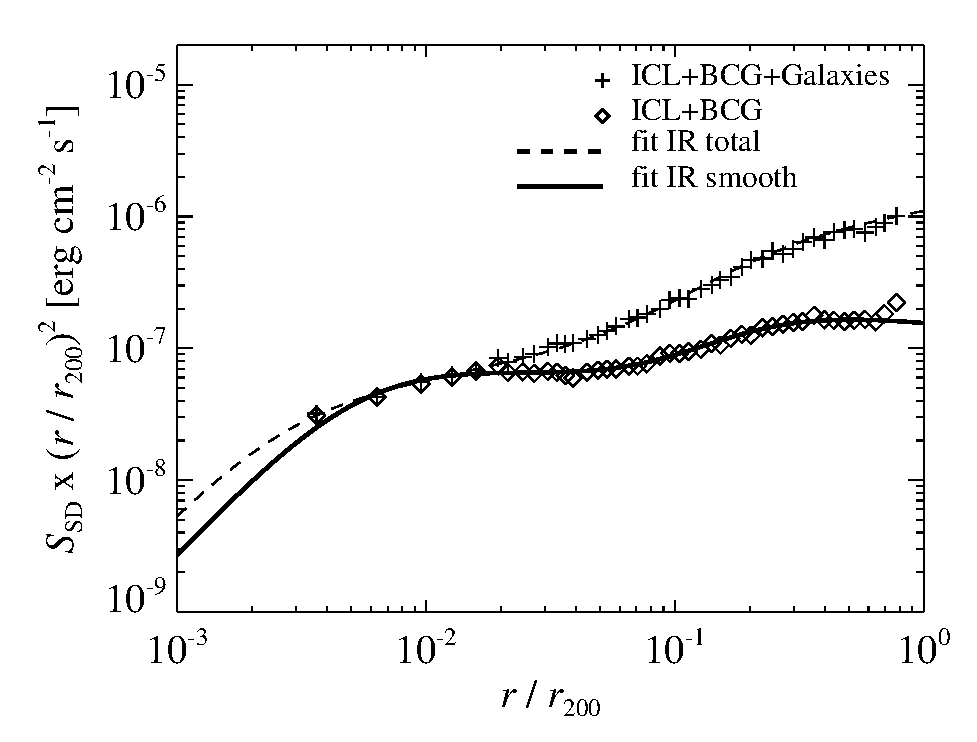
\includegraphics[width=0.99\columnwidth]{figures/SB.photon.eps}
 \caption{\it Surface brightness profiles of the $r$-band $(h\nu\sim
   1\,\ev)$ obtained from stacked clusters in the Sloan Digital Sky
   Survey (SDSS) at the redshift $z \sim 0.25$ \protect
   \cite{2005MNRAS.358..949Z}. The crosses show the total observed
   starlight including the diffuse intracluster light (ICL), galaxies,
   and the brightest cluster galaxy (BCG) in the center of the
   cluster. The diamonds denote the smooth part of the observed
   starlight of the ICL and the BCG. The solid line shows the fit to
   the data of the total light, while the smooth component is
   represented by the dashed line. Note that we use total SD
   brightness in the cluster center, $S_\sd^\rmn{tot}(0)$, to
   normalize the SD surface brightness profiles.}
 \label{fig:SD_spatial}
\end{figure}

Instead of modelling the surface brightness with a de Vaucouleur
profile and a power-law, we use a double beta profile model to
simplify deprojection. It is given by
\begin{equation}
\tilde{S}_\sd (r_\bot) = \frac{S_\sd (r_\bot)}{S_\rmn{SD}^\rmn{tot}(0)} = 
\sum_{i=1}^2 \,\tilde{S}_i\, 
\left[1 + \left( \frac{r_\bot}{r_{\mathrm{c}_i}}\right)^2\right]
^{-3\beta_i + 1/2}.
\label{double_beta}
\end{equation}
Our fit parameters for the normalized central brightness,
$\tilde{S}_i$, the core radius, $r_{\mathrm{c}_i}$, and slope
$\beta_i$ are given for the total model by
\begin{align}
&\tilde{S}_1^\rmn{tot} = 1.0\,,
&&r_{\mathrm{c}_1}^\rmn{tot} = 1.8\,\rmn{kpc}\,,
&&&\beta_1^\rmn{tot} = 0.45\, \nonumber\\
&\tilde{S}_2^\rmn{tot} = 2.3\times10^{-3}\,,
&&r_{\mathrm{c}_2}^\rmn{tot} = 0.19\,\rvir\,,
&&&\beta_2^\rmn{tot} = 0.44\,.\nonumber\\
& && &&&
\label{fit_spatial_IR}
\end{align}
For the smooth model (our benchmark SD model), we find:
\begin{align}
&\tilde{S}_1^\rmn{sm}=0.47,\,
&&r_{\mathrm{c}_1}^\rmn{sm}=3.9\,\rmn{kpc}\,,
&&&\beta_1^\rmn{sm}=0.53 \,\nonumber\\
&\tilde{S}_2^\rmn{sm}=8.3\times10^{-4}\,,
&&r_{\mathrm{c}_2}^\rmn{sm}=0.19\,\rvir\,,
&&&\beta_2^\rmn{sm}=0.54\,.\nonumber\\
& && &&&
\label{fit_spatial_IR_sm}
\end{align}
The three dimensional spatial profile is derived by deprojecting the
surface brightness in Eq.~(\ref{double_beta}) (see
e.g. \cite{2004A&A...413...17P} for details about the deprojection):
\begin{eqnarray}
  j(r)  = \sum_{i=1}^2 \frac{\tilde{S}_i}{2\pi\,r_{\mathrm{c}_i}}\,
  \frac{6 \beta_i - 1}{\left(1 + r^2/r^2_{\mathrm{c}_i}\right)^{3\beta_i}}\,
  \mathcal{B}\left(\frac{1}{2},3\beta_i\right)\,,\nonumber\\
\end{eqnarray}
where $\mathcal{B}(a,b)$ denotes the beta-function
\cite{1965hmfw.book.....A}.

The radial distribution of the energy density of SD governs the seed
photon distribution for IC emission (together with the CMB).  The
energy density from starlight and dust in a galaxy cluster is given by
\begin{eqnarray}
\label{eq:u_SD_r}
u_\sd(r) &=& \int \dd \eph \frac{\dd^2 N_\ph}{\dd \eph \dd V}\,\eph
=\int \dd \eph \frac{u_\sd(\eph, r)}{\eph}
\nonumber \\
&=&  j(r)  \int \dd \eph \sum_i 
N_i(\mvir) \frac{u_i^\gal(\eph)}{\eph}\,, \nonumber \\
\end{eqnarray}
where we have used the specific energy density of the light from SD
given by Eq.~(\ref{eq:u_SD_er}). We compare the energy
density $u_\sd(r)$ to other radiation background fields in
Fig.~\ref{fig:SD_Edens} for a galaxy cluster with the mass
$\mvir=6.0\times10^{14}\msun$. We find that inside a few percent of of
$\rvir$, the total energy density is dominated by the light from SD
while the CMB is dominating elsewhere. This implies that if the boost
from dark matter (DM) substructures is significant, then the overlap of
light from SD with the electron and positron distribution that trace
the substructures is small. Hence the resulting flux from inverse
Compton (IC) upscattered SD photons is suppressed compared to the IC
upscattered CMB photons.

%***********************************************

\section{Source functions of different DM models}
We use {\sc DarkSUSY} to derive the spectral distribution of the
continuum emission from our four DM benchmark (BM) models. These
spectra are shown in the left panel of Fig.~\ref{fig:q_DM}. We choose
to fit the source function in the energy regime $30\,\rmn{MeV}<\eg<
m_\chi c^2$ using the following functional form
\begin{eqnarray}
q_\rmn{BM} (\eg,r)&=&\left[\frac{\rho(r)}{10^{-29}\rmn{g}\,\cm^{-3}}\right]^2
\times\frac{a_1}{\egt}\times\nonumber\\
&\times&\left[\frac{\exp\left(-\egt^{-a_2}\right)}{1+\exp\left(\egt^{a_3}\right)}
+\left(\frac{\egt}{a_4}\right)^{4.5}\right]\,, \nonumber\\
\rmn{where}&\quad& \egt = \frac{\eg}{\gev}\,,
 \label{eq:bm_cont}
\end{eqnarray}
where the model specific parameters are given in
Table~\ref{tab:bm_cont}.

\begin{table}[h]
\begin{tabular}{c c c c c }
\hline
\hline
 BM model & $a_1$ & $a_2$  & $a_3$ & $a_4$ \\
          & $[\gev^{-1}\,\cm^{-2}\,\rmn{s}^{-1}]$ & & & \\
 \hline
$\Ip$ & $2.0\times10^{-4}$ & $0.36$ & $0.51$ & $701$  \\
$\Jp$ & $4.1\times10^{-6}$ & $0.40$ & $0.43$ & $1178$ \\
$\Kp$ & $1.7\times10^{-4}$ & $0.42$ & $0.37$ & $-$    \\
$\Js$ & $2.1\times10^{-6}$ & $0.34$ & $0.51$ & $490$  \\
\hline
\hline
\end{tabular}
\caption{Fit parameters to the continuum emission from our
  supersymmetric benchmark models.
 \label{tab:bm_cont}}
\end{table} 

We also use {\sc DarkSUSY} to derive the number of electrons and
positrons resulting from each annihilation. These spectra are shown in
the right panel of Fig.~\ref{fig:q_DM}. The electron and positron
yield resulting from our supersymmetric BM model is fitted in the
regime $30\,\rmn{MeV}<\ee< m_\chi c^2$ using
\begin{eqnarray}
N_{\e,\rmn{BM}}(>\ee) &=& \frac{b_1}{\eet^{b_2}}\times
\frac{\left[1+\left(\frac{\eet}{b_6}\right)^{b_7}\right]^{b_8}}
{\left[1+\left(\frac{\eet}{b_3}\right)^{b_4}\right]^{b_5}}\,,\nonumber\\
\rmn{where}&\quad&\eet=\frac{\ee}{\gev}\,.
\label{eq:bm_elec}
\end{eqnarray}
Fit parameters are given in Table~\ref{tab:bm_elec}.
\begin{table}[h]
\begin{tabular}{c c c c c c c c c}
\hline
\hline
 BM model & $b_1$ & $b_2$ & $b_3$ & $b_4$ & $b_5$ & $b_6$ & $b_7$ & $b_8$ \\
 \hline
$\Ip$ & $28$ & $0.06$ & $1.8$ & $0.9$  & $2.0$ & $60$  & $5$ & $-1$     \\
$\Jp$ & $34$ & $0.08$ & $5.5$ & $0.8$  & $2.6$ & $250$ & $5$ & $-1$     \\
$\Kp$ & $44$ & $0.05$ & $1.7$ & $0.85$ & $2.1$ & $10$  & $2$ & $0.62$   \\
$\Js$ & $30$ & $0.14$ & $5.0$ & $1.0$  & $1.5$ & $300$ & $5$ & $-1$     \\
\hline
\hline
\end{tabular}
\caption{Fit parameters to the electron and positron yield
  above the electron energy $\ee$ from the supersymmetric benchmark
  models.
 \label{tab:bm_elec}}
\end{table} 

\C{Finally, we use the data from
  \cite{2011JCAP...03..019C,2011JCAP...03..051C} to derive the
  electron and positron yield resulting from leptophilic (LP) DM
  annihilating indirectly into decaying muons or electrons and
  positrons. In the energy regime $30\,\rmn{MeV}<\ee< m_\chi c^2$ we
  find the following best fit for the annihilation into muons:}
\begin{eqnarray}
N_{\e,\rmn{LP}\mu}(>\ee) &=& \exp\left[c_1+c_2\,x+c_3\,(2-x)^{c_4}\right]
\,,\nonumber\\
\rmn{where}\quad x&=&\frac{\ee}{m_\chi\,c^2}\,\quad\rmn{and}\nonumber\\
c_1=1.49,\,c_2&=&-5.00,\,c_3=-2.46,\,c_4=-4.40\,.\nonumber\\
\label{eq:lp_mu}
\end{eqnarray}
Similarly, for the annihilation into electrons and positrons we find the following best fit:
\begin{eqnarray}
N_{\e,\rmn{LP}\e}(>\ee) &=& \exp\left(c_1+c_2\,y+c_3\,y^2\right)
\,,\nonumber\\
\rmn{where}\quad y&=&\,\log\left(1-x\right)\,,\quad 
x=\frac{\ee}{m_\chi\,c^2}\,\quad\rmn{and}\nonumber\\
c_1&=&1.40,\,c_2=1.11,\,c_3=0.058\,.
\label{eq:lp_ep}
\end{eqnarray}

The LP model, that we are using in this work has a branching factor
branching ratio of ($1/4:1/4:1/2$) into
($\mu^+\mu^-:\e^+\e^-:\pi^+\pi^-$). The contribution from the
electrons from the decaying pions is relative small, hence the
resulting electron and positron yield for the LP model is
approximately given by
\begin{equation}
N_{\e,\rmn{LP}}(>\ee) =
N_{\e,\rmn{LP}\e}(>\ee)/4+N_{\e,\rmn{LP}\mu}(>\ee)/4\,.
\end{equation}

\section{Gas density profile of Fornax}
The X-ray emitting gas in Fornax does not follow a simple
$\beta$-profile. Instead, based on deep Rosat data and supported by
Chandra data, it is best modeled by a multicomponent bidimensional
model \cite{2002ApJ...565..883P}, consisting of: (1) a central
component ($r<5\,\kpc$); (2) a ``galactic'' component
($5\,\kpc<r<40\,\kpc$); and (3) an elliptical ICM component
($r>40\,\kpc$). 

In Fig.~\ref{fig:dens_fornax} we show the data points for the electron
number density ($n_\e$) in Fornax, derived from the deep Rosat data
presented in reference \cite{2002ApJ...565..883P}, and the best fit
density profile together with the individual components. The total
$n_\e$ profile is derived from their fitted central and galactic
surface brightness components while we re-fit the ICM component. The
reason for the re-fitted outer component is the large uncertainty in
the data points outside $(0.2-0.3)\rvir$ which we exclude in our
fit. Instead we assume that the outer slop of $n_\e$ follows the outer
slope of Fornax in the HIFLUGCS catalogue that is very similar to that
of the Coma cluster. Deprojecting the fitted surface brightness
components yields the following electron number density profile:
\begin{equation}
n_\e(r) = \left[\sum_i n_i^2\left[1+\left(\frac{r}{r_{c,i}}\right)^2\right]^{-3\beta_i}\right]^{1/2}
\end{equation}
where
\begin{align}
&n_1 = 0.35\, \rmn{el}\,\rmn{cm}^{-3}\,,
&&r_{c,1} = 0.36\,\kpc\,,\,\,\,
\beta_1 = 0.54\,, \nonumber\\
&n_2 = 2.2\times10^{-3}\,\rmn{el}\,\rmn{cm}^{-3}\,,
&&r_{c,2} = 190\,\kpc\,,\,\,\,\,
\beta_2 = 41\,, \nonumber\\
&n_3 = 5.4\times10^{-4}\,\rmn{el}\,\rmn{cm}^{-3}\,,
&&r_{c,3} = 183\,\kpc\,,\,\,\,\,
\beta_3 = 0.8\,. \nonumber\\
& &&
\label{fit_fornax}
\end{align}
Note that we remove the contribution of the flat central component of
the fit ($i=1$) in the outer parts of the cluster, thus we neglect the
central contribution for $r>40\,\kpc$.

\begin{figure}%[t]
 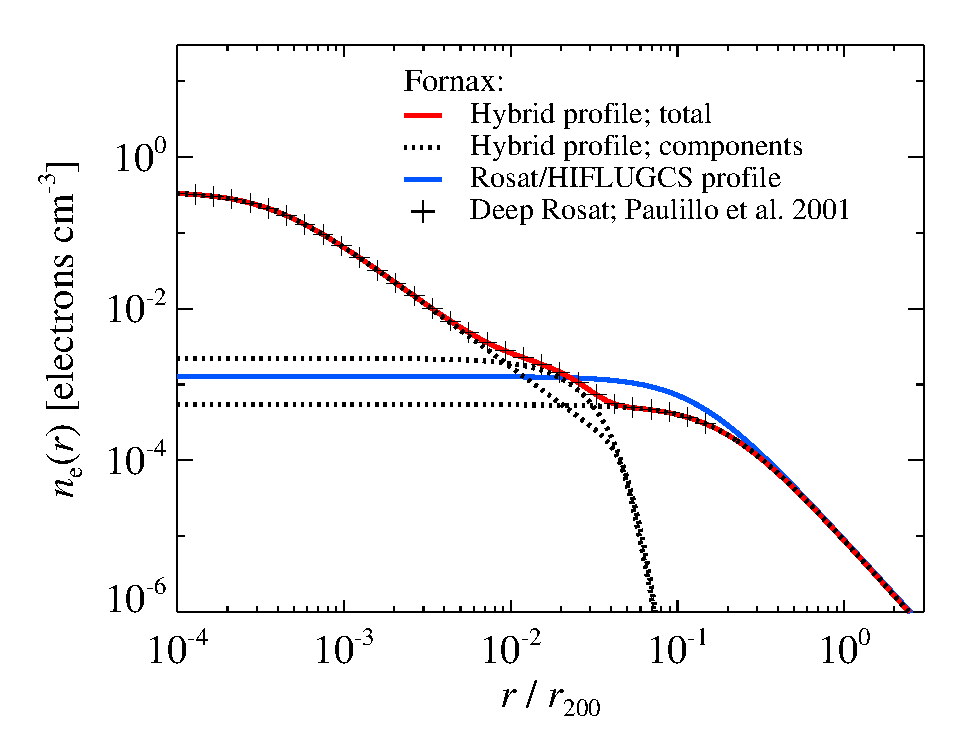
\includegraphics[width=0.99\columnwidth]{figures/dens.fornax.eps}
 \caption{\it Comparing different electron number density profiles for
   the Fornax cluster. Black crosses show the density profile inferred
   from deprojected deep Rosat X-ray surface brightness observations
   \protect \cite{2002ApJ...565..883P}. The total hybrid profile shown
   by the red solid line represent the best fit to the data, where the
   fitted individual density components are shown by the black dotted
   lines. The blue solid line shows the single beta density profile
   inferred from the HIFLUGCS catalogue. Due to insufficient
   sensitivity of the data to the outer cluster part, we use the outer
   slope from the HIFLUGCS catalogue that is very similar to that of
   the Coma cluster.}
 \label{fig:dens_fornax}
\end{figure}


\section{Flux tables for the HIFLUGCS catalogue}

\C{In this section we present the gamma-ray flux predictions using the
  clusters in the extended HIFLUGCS catalogue. We show the brightest
  50 clusters in descending order; CR proton induced $\pi^0$ that
  decays into gamma-rays in Table~\ref{tab:flux_tab_CRs}, the
  supersymmetric DM BM-$\Kp$ model where the Neutralino emit a
  continuum as well as final state radiation in
  Table~\ref{tab:flux_tab_BM}, and LP DM that emit final state
  radiation and annihilate either indirectly to $\rmn{e}^+/\rmn{e}^-$
  or through $\mu^+/\mu^-$ to $\rmn{e}^+/\rmn{e}^-$ that IC upscatter
  CMB photons in Table~\ref{tab:flux_tab_LP}. The flux from DM has
  been boosted by the substructures, where we in addition include the
  Sommerfeld enhancement for the LP model. For completeness, we show
  in Table~\ref{tab:flux_tab_CLp} the parameters that we use to derive
  the fluxes for the clusters in the HIFLUGCS sample.}

\begin{table*}
\begin{minipage}{2.0\columnwidth}
  \caption{Gamma-ray CR-$\pi^0$ flux within $\rvir$ from brightest 50 clusters in HIFLUGCS catalogue.}
\begin{tabular}{l  c c c c c c c}
\hline
\hline
 Cluster & ID$^{(1)}$ & $F_{\gamma}$$^{(2)}$ & $F_{\gamma}$$^{(3)}$& 
 $F_{\gamma}$$^{(4)}$ & $\eg^2\,\dd F_{\gamma}/\dd \eg$$^{(5)}$ &
 $\eg^2\,\dd F_{\gamma,0.1}/\dd \eg$$^{(5,6)}$ & 
 $\eg^2\,\dd F_{\gamma,1.0}/\dd \eg$$^{(5,7)}$\\
  & & $(>100\,\rmn{MeV})$ & $(>1\,\rmn{GeV})$ & $(>100\,\rmn{GeV})$ & 
 $(5\,\rmn{GeV})$ & $(5\,\rmn{GeV})$ &  $(5\,\rmn{GeV})$\\
 \hline
PERSEUS  &  68 &  56.14 &  75.31 &  20.64 &  63.95 &  13.92 &  24.52 \\
OPHIUCHUS &  96 &  23.31 &  31.27 &   8.57 &  26.55 &   5.88 &  10.28 \\
COMA     &  34 &  17.50 &  23.48 &   6.43 &  19.94 &   2.62 &   7.56 \\
NORMA    &  94 &  13.39 &  17.97 &   4.92 &  15.26 &   1.16 &   5.57 \\
CENTAURUS &  30 &  12.06 &  16.17 &   4.43 &  13.73 &   2.45 &   5.04 \\
AWM7     &  67 &   8.24 &  11.05 &   3.03 &   9.38 &   1.85 &   3.63 \\
A3571    &  39 &   6.10 &   8.19 &   2.24 &   6.95 &   1.80 &   2.83 \\
TRIANGULUM &  95 &   5.92 &   7.95 &   2.18 &   6.75 &   1.61 &   2.81 \\
A2319    &  98 &   5.58 &   7.48 &   2.05 &   6.35 &   1.54 &   2.74 \\
A2199    &  51 &   5.18 &   6.94 &   1.90 &   5.90 &   1.68 &   2.35 \\
3C129    &  70 &   5.15 &   6.91 &   1.89 &   5.87 &   0.71 &   2.30 \\
HYDRA    &  25 &   5.15 &   6.91 &   1.89 &   5.86 &   1.11 &   2.22 \\
2A0335   &  11 &   4.91 &   6.59 &   1.81 &   5.59 &   1.94 &   2.33 \\
FORNAX   &  10 &   4.09 &   5.48 &   1.50 &   4.66 &   0.33 &   1.65 \\
A2029    &  43 &   3.73 &   5.00 &   1.37 &   4.25 &   1.45 &   1.80 \\
A0496    &  18 &   3.59 &   4.81 &   1.32 &   4.09 &   1.13 &   1.84 \\
A0085    &   1 &   3.54 &   4.75 &   1.30 &   4.04 &   1.20 &   1.79 \\
A1795    &  40 &   3.52 &   4.73 &   1.29 &   4.01 &   1.37 &   1.66 \\
A2256    &  54 &   3.45 &   4.63 &   1.27 &   3.93 &   1.11 &   1.55 \\
PKS0745  &  77 &   3.28 &   4.40 &   1.20 &   3.73 &   1.39 &   1.57 \\
A3266    &  17 &   3.18 &   4.27 &   1.17 &   3.63 &   0.92 &   1.45 \\
A2142    &  48 &   3.09 &   4.14 &   1.13 &   3.52 &   1.16 &   1.50 \\
NGC5044  &  35 &   2.97 &   3.98 &   1.09 &   3.38 &   1.01 &   1.34 \\
A3558    &  37 &   2.89 &   3.88 &   1.06 &   3.29 &   0.82 &   1.44 \\
A3667    &  56 &   2.85 &   3.82 &   1.05 &   3.25 &   0.73 &   1.55 \\
A0262    &   5 &   2.76 &   3.70 &   1.01 &   3.14 &   0.57 &   1.41 \\
A0478    &  14 &   2.72 &   3.64 &   1.00 &   3.09 &   1.11 &   1.30 \\
A1367    &  26 &   2.65 &   3.55 &   0.97 &   3.02 &   0.40 &   1.19 \\
A4038    &  62 &   2.56 &   3.43 &   0.94 &   2.91 &   0.83 &   1.22 \\
HYDRA-A  &  24 &   2.46 &   3.30 &   0.90 &   2.80 &   0.98 &   1.19 \\
A0401    &   8 &   2.39 &   3.21 &   0.88 &   2.72 &   0.82 &   1.16 \\
A2052    &  44 &   2.25 &   3.02 &   0.83 &   2.57 &   0.81 &   1.11 \\
A0644    &  78 &   2.17 &   2.91 &   0.80 &   2.47 &   0.84 &   0.98 \\
NGC1550  &  15 &   2.06 &   2.76 &   0.76 &   2.35 &   0.59 &   0.93 \\
NGC4636  &  29 &   2.06 &   2.76 &   0.76 &   2.34 &   0.55 &   0.86 \\
A0754    &  23 &   2.03 &   2.73 &   0.75 &   2.32 &   0.69 &   0.92 \\
ANTLIA   &  79 &   1.87 &   2.50 &   0.69 &   2.13 &   0.19 &   0.82 \\
A3158    &  13 &   1.83 &   2.45 &   0.67 &   2.08 &   0.61 &   0.86 \\
A2147    &  49 &   1.80 &   2.41 &   0.66 &   2.05 &   0.29 &   1.19 \\
A0119    &   2 &   1.75 &   2.35 &   0.65 &   2.00 &   0.38 &   0.84 \\
A2063    &  47 &   1.70 &   2.28 &   0.63 &   1.94 &   0.53 &   0.82 \\
A3581    &  41 &   1.66 &   2.22 &   0.61 &   1.89 &   0.58 &   0.78 \\
A1644    &  31 &   1.63 &   2.19 &   0.60 &   1.86 &   0.42 &   0.85 \\
MKW3S    &  45 &   1.62 &   2.18 &   0.60 &   1.85 &   0.62 &   0.77 \\
A2065    &  46 &   1.56 &   2.09 &   0.57 &   1.78 &   0.58 &   0.70 \\
A0399    &   7 &   1.55 &   2.07 &   0.57 &   1.76 &   0.50 &   0.73 \\
A3112    &   9 &   1.54 &   2.07 &   0.57 &   1.76 &   0.63 &   0.76 \\
EXO0422  &  16 &   1.53 &   2.05 &   0.56 &   1.74 &   0.58 &   0.69 \\
A4059    &  63 &   1.51 &   2.02 &   0.55 &   1.72 &   0.54 &   0.72 \\
A0576    &  22 &   1.47 &   1.97 &   0.54 &   1.68 &   0.42 &   0.66 \\
\hline
\hline
\end{tabular}
\begin{quote}
  Notes: 
   (1) The HIFLUGCS cluster ID.
   (2) In units of  $10^{-10} \rmn{ph}\,\rmn{cm}^{-2}\,\rmn{s}^{-1}$.
   (3) In units of  $10^{-11} \rmn{ph}\,\rmn{cm}^{-2}\,\rmn{s}^{-1}$.
   (4) In units of  $10^{-13} \rmn{ph}\,\rmn{cm}^{-2}\,\rmn{s}^{-1}$.
   (5) In units of  $10^{-11} \rmn{erg}\,\rmn{cm}^{-2}\,\rmn{s}^{-1}$.
   (6) The flux within $0.1$ degree. In addition, we smooth the flux with a point spread function of $0.1$ degree. 
   (7) The flux within $1.0$ degree. In addition, we smooth the flux with a point spread function of $1.0$ degree. 
 \label{tab:flux_tab_CRs}
  \end{quote}
\end{minipage}
\end{table*} 

\begin{table*}
\begin{minipage}{2.0\columnwidth}
  \caption{Gamma-ray BM-$\Kp$ Continuum flux within $\rvir$ from brightest 50 clusters in HIFLUGCS catalogue.}
\begin{tabular}{l  c c c c c c c}
\hline
\hline
 Cluster & ID$^{(1)}$ & $F_{\gamma}$$^{(2)}$ & $F_{\gamma}$$^{(3)}$& 
 $F_{\gamma}$$^{(4)}$ & $\eg^2\,\dd F_{\gamma}/\dd \eg$$^{(5)}$ &
 $\eg^2\,\dd F_{\gamma,0.1}/\dd \eg$$^{(5,6)}$ & 
 $\eg^2\,\dd F_{\gamma,1.0}/\dd \eg$$^{(5,7)}$\\
  & & $(>100\,\rmn{MeV})$ & $(>1\,\rmn{GeV})$ & $(>100\,\rmn{GeV})$ & 
 $(5\,\rmn{GeV})$ & $(5\,\rmn{GeV})$ &  $(5\,\rmn{GeV})$\\
 \hline
FORNAX   &  10 &  12.71 &  80.57 &  44.45 &  12.76 &   0.09 &   2.61 \\
OPHIUCHUS &  96 &   9.95 &  63.10 &  34.81 &   9.99 &   0.27 &   3.90 \\
COMA     &  34 &   8.26 &  52.38 &  28.89 &   8.29 &   0.22 &   3.20 \\
NORMA    &  94 &   7.48 &  47.43 &  26.16 &   7.51 &   0.17 &   2.68 \\
CENTAURUS &  30 &   7.24 &  45.87 &  25.31 &   7.26 &   0.12 &   2.28 \\
PERSEUS  &  68 &   7.15 &  45.30 &  24.99 &   7.17 &   0.18 &   2.67 \\
HYDRA    &  25 &   6.75 &  42.81 &  23.61 &   6.78 &   0.12 &   2.23 \\
M49      &  81 &   5.98 &  37.93 &  20.92 &   6.00 &   0.06 &   1.51 \\
NGC4636  &  29 &   4.42 &  28.01 &  15.45 &   4.44 &   0.05 &   1.14 \\
AWM7     &  67 &   4.30 &  27.24 &  15.03 &   4.31 &   0.13 &   1.76 \\
3C129    &  70 &   4.06 &  25.74 &  14.20 &   4.08 &   0.15 &   1.79 \\
A1367    &  26 &   2.51 &  15.92 &   8.78 &   2.52 &   0.11 &   1.20 \\
NGC5846  &  92 &   2.48 &  15.73 &   8.68 &   2.49 &   0.05 &   0.86 \\
A0754    &  23 &   2.14 &  13.57 &   7.49 &   2.15 &   0.17 &   1.26 \\
TRIANGULUM &  95 &   1.85 &  11.72 &   6.47 &   1.86 &   0.16 &   1.10 \\
A3571    &  39 &   1.84 &  11.68 &   6.45 &   1.85 &   0.14 &   1.05 \\
NGC5813  &  91 &   1.59 &  10.06 &   5.55 &   1.59 &   0.04 &   0.62 \\
ANTLIA   &  79 &   1.58 &  10.03 &   5.53 &   1.59 &   0.06 &   0.71 \\
A2199    &  51 &   1.54 &   9.73 &   5.37 &   1.54 &   0.11 &   0.85 \\
A3266    &  17 &   1.50 &   9.49 &   5.24 &   1.50 &   0.15 &   0.94 \\
A2877    &  65 &   1.48 &   9.40 &   5.18 &   1.49 &   0.09 &   0.79 \\
NGC5044  &  35 &   1.42 &   9.00 &   4.97 &   1.43 &   0.05 &   0.61 \\
A3395n   &  75 &   1.35 &   8.57 &   4.73 &   1.36 &   0.13 &   0.83 \\
A3395s   &  21 &   1.35 &   8.56 &   4.72 &   1.36 &   0.13 &   0.83 \\
A2256    &  54 &   1.34 &   8.49 &   4.68 &   1.34 &   0.14 &   0.85 \\
A0576    &  22 &   1.31 &   8.28 &   4.57 &   1.31 &   0.11 &   0.77 \\
NGC1550  &  15 &   1.30 &   8.25 &   4.55 &   1.31 &   0.06 &   0.62 \\
A2319    &  98 &   1.25 &   7.92 &   4.37 &   1.25 &   0.13 &   0.80 \\
A3376    &  19 &   1.24 &   7.85 &   4.33 &   1.24 &   0.12 &   0.76 \\
A0119    &   2 &   1.19 &   7.54 &   4.16 &   1.19 &   0.11 &   0.73 \\
A2634    &  60 &   1.11 &   7.07 &   3.90 &   1.12 &   0.09 &   0.65 \\
A0262    &   5 &   1.02 &   6.46 &   3.57 &   1.02 &   0.06 &   0.53 \\
A2065    &  46 &   0.98 &   6.21 &   3.42 &   0.98 &   0.13 &   0.67 \\
A0539    &  71 &   0.90 &   5.70 &   3.14 &   0.90 &   0.08 &   0.53 \\
MKW8     &  42 &   0.89 &   5.65 &   3.12 &   0.89 &   0.07 &   0.52 \\
A1795    &  40 &   0.87 &   5.50 &   3.03 &   0.87 &   0.11 &   0.58 \\
A0644    &  78 &   0.85 &   5.42 &   2.99 &   0.86 &   0.11 &   0.59 \\
A4038    &  62 &   0.82 &   5.23 &   2.88 &   0.83 &   0.07 &   0.49 \\
A0496    &  18 &   0.80 &   5.09 &   2.81 &   0.81 &   0.08 &   0.49 \\
IIIZw54  &  12 &   0.80 &   5.05 &   2.79 &   0.80 &   0.07 &   0.49 \\
A2147    &  49 &   0.78 &   4.97 &   2.74 &   0.79 &   0.08 &   0.49 \\
A3558    &  37 &   0.77 &   4.88 &   2.69 &   0.77 &   0.09 &   0.51 \\
A3667    &  56 &   0.75 &   4.74 &   2.62 &   0.75 &   0.09 &   0.51 \\
A0085    &   1 &   0.73 &   4.64 &   2.56 &   0.73 &   0.09 &   0.50 \\
A2063    &  47 &   0.72 &   4.58 &   2.52 &   0.72 &   0.07 &   0.46 \\
A0399    &   7 &   0.69 &   4.39 &   2.42 &   0.69 &   0.10 &   0.49 \\
UGC03957 &  76 &   0.69 &   4.35 &   2.40 &   0.69 &   0.07 &   0.43 \\
A2029    &  43 &   0.68 &   4.34 &   2.39 &   0.69 &   0.10 &   0.49 \\
A0400    &   6 &   0.68 &   4.31 &   2.38 &   0.68 &   0.06 &   0.41 \\
A3158    &  13 &   0.67 &   4.26 &   2.35 &   0.67 &   0.09 &   0.46 \\
\hline
\hline
\end{tabular}
\begin{quote}
  Notes: 
   (1) The HIFLUGCS cluster ID.
   (2) In units of  $10^{-11} \rmn{ph}\,\rmn{cm}^{-2}\,\rmn{s}^{-1}$.
   (3) In units of  $10^{-12} \rmn{ph}\,\rmn{cm}^{-2}\,\rmn{s}^{-1}$.
   (4) In units of  $10^{-14} \rmn{ph}\,\rmn{cm}^{-2}\,\rmn{s}^{-1}$.
   (5) In units of  $10^{-11} \rmn{erg}\,\rmn{cm}^{-2}\,\rmn{s}^{-1}$.
   (6) The flux within $0.1$ degree. In addition, we smooth the flux with a point spread function of $0.1$ degree. 
   (7) The flux within $1.0$ degree. In addition, we smooth the flux with a point spread function of $1.0$ degree. 
  \label{tab:flux_tab_BM}
  \end{quote}
\end{minipage}
\end{table*} 


\begin{table*}
\begin{minipage}{2.0\columnwidth}
  \caption{Gamma-ray LP-IC-CMB and LP-BS flux within $\rvir$ from brightest 50 clusters in HIFLUGCS catalogue.}
\begin{tabular}{l  c c c c c c c}
\hline
\hline
 Cluster & ID$^{(1)}$ & $F_{\gamma}$$^{(2)}$ & $F_{\gamma}$$^{(3)}$& 
 $F_{\gamma}$$^{(4)}$ & $\eg^2\,\dd F_{\gamma}/\dd \eg$$^{(5)}$ &
 $\eg^2\,\dd F_{\gamma,0.1}/\dd \eg$$^{(5,6)}$ & 
 $\eg^2\,\dd F_{\gamma,1.0}/\dd \eg$$^{(5,7)}$\\
  & & $(>100\,\rmn{MeV})$ & $(>1\,\rmn{GeV})$ & $(>100\,\rmn{GeV})$ & 
 $(5\,\rmn{GeV})$ & $(5\,\rmn{GeV})$ &  $(5\,\rmn{GeV})$\\
 \hline
FORNAX   &  10 &  13.70 &  17.37 &  20.12 &  16.99 &   0.05 &   1.91 \\
OPHIUCHU &  96 &  11.00 &  13.95 &  15.76 &  13.64 &   0.20 &   3.01 \\
COMA     &  34 &   8.97 &  11.38 &  13.08 &  11.13 &   0.15 &   2.42 \\
CENTAURU &  30 &   8.00 &  10.14 &  11.46 &   9.92 &   0.08 &   1.75 \\
NORMA    &  94 &   7.98 &  10.11 &  11.85 &   9.89 &   0.10 &   1.99 \\
PERSEUS  &  68 &   7.93 &  10.06 &  11.31 &   9.83 &   0.13 &   2.07 \\
HYDRA    &  25 &   7.44 &   9.43 &  10.69 &   9.22 &   0.09 &   1.71 \\
M49      &  81 &   6.53 &   8.28 &   9.47 &   8.10 &   0.04 &   1.13 \\
NGC4636  &  29 &   4.78 &   6.06 &   7.00 &   5.93 &   0.03 &   0.85 \\
AWM7     &  67 &   4.71 &   5.97 &   6.80 &   5.84 &   0.09 &   1.34 \\
3C129    &  70 &   4.34 &   5.51 &   6.43 &   5.38 &   0.10 &   1.34 \\
NGC5846  &  92 &   2.70 &   3.42 &   3.93 &   3.35 &   0.03 &   0.65 \\
A1367    &  26 &   2.64 &   3.35 &   3.98 &   3.28 &   0.07 &   0.89 \\
A0754    &  23 &   2.37 &   3.00 &   3.39 &   2.93 &   0.13 &   0.97 \\
A3571    &  39 &   2.03 &   2.57 &   2.92 &   2.52 &   0.10 &   0.81 \\
TRIANGUL &  95 &   2.02 &   2.56 &   2.93 &   2.51 &   0.11 &   0.85 \\
NGC5813  &  91 &   1.72 &   2.18 &   2.51 &   2.13 &   0.03 &   0.47 \\
A2199    &  51 &   1.69 &   2.14 &   2.43 &   2.10 &   0.08 &   0.66 \\
A3266    &  17 &   1.61 &   2.04 &   2.37 &   1.99 &   0.10 &   0.72 \\
A2877    &  65 &   1.60 &   2.03 &   2.35 &   1.98 &   0.06 &   0.60 \\
ANTLIA   &  79 &   1.60 &   2.02 &   2.51 &   1.98 &   0.03 &   0.51 \\
NGC5044  &  35 &   1.55 &   1.96 &   2.25 &   1.92 &   0.03 &   0.47 \\
A3395s   &  21 &   1.45 &   1.83 &   2.14 &   1.79 &   0.09 &   0.63 \\
A2256    &  54 &   1.44 &   1.83 &   2.12 &   1.79 &   0.10 &   0.65 \\
A3395n   &  75 &   1.44 &   1.82 &   2.14 &   1.78 &   0.09 &   0.63 \\
NGC1550  &  15 &   1.42 &   1.80 &   2.06 &   1.76 &   0.04 &   0.47 \\
A0576    &  22 &   1.41 &   1.78 &   2.07 &   1.74 &   0.08 &   0.59 \\
A2319    &  98 &   1.36 &   1.72 &   1.98 &   1.69 &   0.09 &   0.61 \\
A3376    &  19 &   1.30 &   1.65 &   1.96 &   1.61 &   0.08 &   0.57 \\
A0119    &   2 &   1.24 &   1.58 &   1.88 &   1.54 &   0.07 &   0.55 \\
A2634    &  60 &   1.17 &   1.48 &   1.77 &   1.45 &   0.06 &   0.49 \\
A0262    &   5 &   1.11 &   1.41 &   1.61 &   1.38 &   0.04 &   0.41 \\
A2065    &  46 &   1.06 &   1.34 &   1.55 &   1.31 &   0.09 &   0.51 \\
A0539    &  71 &   0.98 &   1.24 &   1.42 &   1.21 &   0.05 &   0.41 \\
MKW8     &  42 &   0.97 &   1.23 &   1.41 &   1.20 &   0.05 &   0.40 \\
A1795    &  40 &   0.96 &   1.22 &   1.37 &   1.20 &   0.08 &   0.45 \\
A0644    &  78 &   0.94 &   1.20 &   1.35 &   1.17 &   0.09 &   0.46 \\
A4038    &  62 &   0.91 &   1.15 &   1.31 &   1.13 &   0.05 &   0.38 \\
A0496    &  18 &   0.89 &   1.13 &   1.27 &   1.10 &   0.06 &   0.38 \\
IIIZw54  &  12 &   0.86 &   1.09 &   1.26 &   1.07 &   0.05 &   0.37 \\
A3558    &  37 &   0.84 &   1.06 &   1.22 &   1.04 &   0.06 &   0.39 \\
A2147    &  49 &   0.82 &   1.04 &   1.24 &   1.01 &   0.05 &   0.37 \\
A0085    &   1 &   0.81 &   1.03 &   1.16 &   1.01 &   0.07 &   0.38 \\
A3667    &  56 &   0.80 &   1.02 &   1.19 &   1.00 &   0.07 &   0.38 \\
A2063    &  47 &   0.79 &   1.00 &   1.14 &   0.98 &   0.05 &   0.35 \\
A2029    &  43 &   0.76 &   0.96 &   1.08 &   0.94 &   0.08 &   0.38 \\
UGC03957 &  76 &   0.75 &   0.96 &   1.09 &   0.93 &   0.05 &   0.33 \\
A0399    &   7 &   0.74 &   0.94 &   1.10 &   0.92 &   0.07 &   0.37 \\
A3158    &  13 &   0.73 &   0.93 &   1.06 &   0.91 &   0.07 &   0.36 \\
A0400    &   6 &   0.73 &   0.92 &   1.08 &   0.90 &   0.04 &   0.31 \\
\hline
\hline
\end{tabular}
\begin{quote}
  Notes: 
   (1) The HIFLUGCS cluster ID.
   (2) In units of  $10^{-8} \rmn{ph}\,\rmn{cm}^{-2}\,\rmn{s}^{-1}$.
   (3) In units of  $10^{-9} \rmn{ph}\,\rmn{cm}^{-2}\,\rmn{s}^{-1}$.
   (4) In units of  $10^{-12} \rmn{ph}\,\rmn{cm}^{-2}\,\rmn{s}^{-1}$.
   (5) In units of  $10^{-9} \rmn{erg}\,\rmn{cm}^{-2}\,\rmn{s}^{-1}$.
   (6) The flux within $0.1$ degree that have in addition been smoothed over with a point spread function of $0.1$ degree. 
   (7) The flux within $1.0$ degree that have in addition been smoothed over with a point spread function of $1.0$ degree. 
 \label{tab:flux_tab_LP}
  \end{quote}
\end{minipage}
\end{table*} 

\begin{table*}
\begin{minipage}{2.0\columnwidth}
  \caption{Galaxy cluster parameters for to all clusters in the HIFLUGCS catalogue.}
\begin{tabular}{l  c c c c c c c c c c c}
\hline
\hline
Cluster & ID$^{(1)}$ & $D_\clu$$^{(1)}$ & $\rvir$$^{(1)}$ & $\rvir$ & 
$\mvir$$^{(1)}$ & $\rho_\rmn{gas}(0)$$^{(2)}$ & $r_\rmn{core}$$^{(2)}$ & 
$\beta$$^{(2)}$ & $r_\rmn{hlr,CR}$$^{(3)}$ & $r_\rmn{hlr,DM}$  $^{(4)}$ \\
& & [Mpc] & [Mpc] & [deg] & [$10^{14}\,\msun$] & 
[$10^{-27}\,\rmn{g}\,\rmn{cm}^{-3}$] & [kpc] &  & [deg] & [deg] \\
 \hline
A0085    &   1 & 248.29 &   1.90 &   0.44 &   7.71 &  24.54 &  59.29 &   0.53 &   0.04 &   0.20 \\
A0119    &   2 & 194.82 &   1.90 &   0.56 &   7.69 &   1.93 & 357.86 &   0.68 &   0.13 &   0.26 \\
A0133    &   3 & 254.34 &   1.41 &   0.32 &   3.15 &  35.76 &  32.14 &   0.53 &   0.02 &   0.15 \\
NGC507   &   4 &  71.57 &   0.74 &   0.59 &   0.46 &  23.05 &  13.57 &   0.44 &   0.07 &   0.28 \\
A0262    &   5 &  69.81 &   0.96 &   0.79 &   1.01 &  14.38 &  30.00 &   0.44 &   0.14 &   0.37 \\
A0400    &   6 & 104.69 &   1.09 &   0.60 &   1.48 &   3.40 & 110.00 &   0.53 &   0.12 &   0.28 \\
A0399    &   7 & 323.00 &   2.19 &   0.39 &  11.89 &   3.40 & 321.43 &   0.71 &   0.07 &   0.18 \\
A0401    &   8 & 338.70 &   2.19 &   0.37 &  11.85 &   7.84 & 175.71 &   0.61 &   0.05 &   0.17 \\
A3112    &   9 & 339.66 &   1.74 &   0.29 &   5.87 &  43.07 &  43.57 &   0.58 &   0.02 &   0.14 \\
FORNAX   &  10 &  19.77 &   0.96 &   2.79 &   1.01 &   2.48 & 124.29 &   0.80 &   0.31 &   1.30 \\
2A0335   &  11 & 153.49 &   1.31 &   0.49 &   2.51 &  93.06 &  23.57 &   0.57 &   0.02 &   0.23 \\
IIIZw54  &  12 & 136.39 &   1.35 &   0.57 &   2.81 &   3.86 & 206.43 &   0.89 &   0.07 &   0.26 \\
A3158    &  13 & 264.13 &   1.92 &   0.42 &   8.06 &   5.96 & 192.14 &   0.66 &   0.06 &   0.19 \\
A0478    &  14 & 411.96 &   2.24 &   0.31 &  12.78 &  35.47 &  70.00 &   0.61 &   0.02 &   0.14 \\
NGC1550  &  15 &  53.18 &   0.88 &   0.95 &   0.78 &  15.86 &  32.14 &   0.55 &   0.07 &   0.44 \\
EXO0422  &  16 & 172.04 &   1.43 &   0.48 &   3.31 &  11.91 & 101.43 &   0.72 &   0.04 &   0.22 \\
A3266    &  17 & 266.00 &   2.46 &   0.53 &  16.97 &   3.17 & 402.86 &   0.80 &   0.08 &   0.25 \\
A0496    &  18 & 144.03 &   1.40 &   0.56 &   3.11 &  51.30 &  21.43 &   0.48 &   0.05 &   0.26 \\
A3376    &  19 & 201.69 &   1.96 &   0.56 &   8.54 &   1.70 & 539.29 &   1.05 &   0.10 &   0.26 \\
A3391    &  20 & 236.69 &   1.74 &   0.42 &   6.01 &   3.93 & 167.14 &   0.58 &   0.07 &   0.20 \\
A3395s   &  21 & 221.45 &   2.14 &   0.55 &  10.96 &   2.07 & 431.43 &   0.96 &   0.08 &   0.26 \\
A0576    &  22 & 167.96 &   1.79 &   0.61 &   6.40 &   2.97 & 281.43 &   0.82 &   0.08 &   0.28 \\
A0754    &  23 & 235.31 &   2.55 &   0.62 &  18.71 &   5.98 & 170.71 &   0.70 &   0.05 &   0.29 \\
HYDRA-A  &  24 & 239.94 &   1.55 &   0.37 &   4.24 &  53.04 &  35.71 &   0.57 &   0.02 &   0.17 \\
HYDRA    &  25 &  49.25 &   1.39 &   1.62 &   3.03 &   8.20 &  67.14 &   0.61 &   0.13 &   0.75 \\
A1367    &  26 &  94.05 &   1.53 &   0.93 &   4.06 &   2.02 & 273.57 &   0.69 &   0.19 &   0.43 \\
MKW4     &  27 &  86.98 &   0.86 &   0.56 &   0.71 &  50.43 &   7.86 &   0.44 &   0.06 &   0.26 \\
ZwCl1215 &  28 & 339.66 &   2.09 &   0.35 &  10.37 &   4.07 & 307.86 &   0.82 &   0.05 &   0.16 \\
NGC4636  &  29 &  15.89 &   0.61 &   2.19 &   0.25 &  55.18 &   4.29 &   0.49 &   0.07 &   1.02 \\
CENTAURU &  30 &  44.46 &   1.34 &   1.72 &   2.70 &  24.45 &  26.43 &   0.49 &   0.14 &   0.80 \\
A1644    &  31 & 210.40 &   1.62 &   0.44 &   4.81 &   3.49 & 214.29 &   0.58 &   0.10 &   0.21 \\
A1650    &  32 & 385.28 &   2.15 &   0.32 &  11.14 &   6.77 & 200.71 &   0.70 &   0.04 &   0.15 \\
A1651    &  33 & 392.54 &   1.96 &   0.29 &   8.51 &  11.72 & 129.29 &   0.64 &   0.03 &   0.13 \\
COMA     &  34 & 101.14 &   2.30 &   1.30 &  13.84 &   4.34 & 245.71 &   0.65 &   0.20 &   0.60 \\
NGC5044  &  35 &  38.81 &   0.74 &   1.10 &   0.46 &  81.77 &   7.86 &   0.52 &   0.03 &   0.51 \\
A1736    &  36 & 204.44 &   1.34 &   0.37 &   2.70 &   2.10 & 267.14 &   0.54 &   0.12 &   0.17 \\
A3558    &  37 & 213.16 &   1.76 &   0.47 &   6.17 &   6.51 & 160.00 &   0.58 &   0.08 &   0.22 \\
A3562    &  38 & 221.91 &   1.54 &   0.40 &   4.16 &   8.30 &  70.71 &   0.47 &   0.08 &   0.18 \\
A3571    &  39 & 175.22 &   2.04 &   0.67 &   9.51 &  10.39 & 129.29 &   0.61 &   0.07 &   0.31 \\
A1795    &  40 & 276.29 &   2.14 &   0.44 &  10.99 &  35.96 &  55.71 &   0.60 &   0.02 &   0.21 \\
A3581    &  41 &  93.17 &   0.99 &   0.61 &   1.09 &  31.10 &  25.00 &   0.54 &   0.03 &   0.28 \\
MKW8     &  42 & 118.04 &   1.28 &   0.62 &   2.38 &   5.06 &  76.43 &   0.51 &   0.10 &   0.29 \\
A2029    &  43 & 347.78 &   2.29 &   0.38 &  13.42 &  38.80 &  59.29 &   0.58 &   0.02 &   0.17 \\
A2052    &  44 & 153.04 &   1.25 &   0.47 &   2.21 &  44.71 &  26.43 &   0.53 &   0.03 &   0.22 \\
MKW3S    &  45 & 199.40 &   1.45 &   0.42 &   3.46 &  26.57 &  47.14 &   0.58 &   0.02 &   0.19 \\
A2065    &  46 & 325.85 &   2.45 &   0.43 &  16.69 &   3.31 & 492.86 &   1.16 &   0.05 &   0.20 \\
A2063    &  47 & 155.75 &   1.42 &   0.52 &   3.24 &  10.17 &  78.57 &   0.56 &   0.06 &   0.24 \\
A2142    &  48 & 411.47 &   2.36 &   0.33 &  15.03 &  18.05 & 110.00 &   0.59 &   0.03 &   0.15 \\
A2147    &  49 & 154.39 &   1.45 &   0.54 &   3.46 &   2.41 & 170.00 &   0.44 &   0.18 &   0.25 \\
A2163    &  50 & 990.91 &   3.21 &   0.19 &  37.14 &   6.43 & 370.71 &   0.80 &   0.02 &   0.09 \\
A2199    &  51 & 132.35 &   1.62 &   0.70 &   4.81 &  13.66 &  99.29 &   0.66 &   0.06 &   0.33 \\
A2204    &  52 & 727.47 &   2.06 &   0.16 &   9.85 &  73.26 &  47.86 &   0.60 &   0.01 &   0.08 \\
A2244    &  53 & 446.19 &   2.06 &   0.27 &   9.84 &  17.26 &  90.00 &   0.61 &   0.02 &   0.12 \\
A2256    &  54 & 269.27 &   2.40 &   0.51 &  15.58 &   3.90 & 419.29 &   0.91 &   0.07 &   0.24 \\
A2255    &  55 & 363.60 &   2.27 &   0.36 &  13.32 &   2.40 & 423.57 &   0.80 &   0.06 &   0.17 \\
\end{tabular}
 \label{tab:flux_tab_CLp}
\end{minipage}
\end{table*} 
\newpage
\begin{table}
\begin{minipage}{2.0\columnwidth}
\begin{tabular}{l  c c c c c c c c c c c}
\hline
\hline
Cluster & ID$^{(1)}$ & $D_\clu$$^{(1)}$ & $\rvir$$^{(1)}$ & $\rvir$ & 
$\mvir$$^{(1)}$ & $\rho_\rmn{gas}(0)$$^{(2)}$ & $r_\rmn{core}$$^{(2)}$ & 
$\beta$$^{(2)}$ & $r_\rmn{hlr,CR}$$^{(3)}$ & $r_\rmn{hlr,DM}$  $^{(4)}$ \\
& & [Mpc] & [Mpc] & [deg] & [$10^{14}\,\msun$] & 
[$10^{-27}\,\rmn{g}\,\rmn{cm}^{-3}$] & [kpc] &  & [deg] & [deg] \\
 \hline
A3667    &  56 & 250.15 &   1.92 &   0.44 &   7.99 &   4.64 & 199.29 &   0.54 &   0.10 &   0.20 \\
S1101    &  57 & 259.46 &   1.37 &   0.30 &   2.91 &  48.52 &  40.00 &   0.64 &   0.01 &   0.14 \\
A2589    &  58 & 183.87 &   1.47 &   0.46 &   3.58 &  10.07 &  84.29 &   0.60 &   0.04 &   0.21 \\
A2597    &  59 & 388.66 &   1.65 &   0.24 &   5.10 &  59.06 &  41.43 &   0.63 &   0.01 &   0.11 \\
A2634    &  60 & 136.84 &   1.50 &   0.63 &   3.82 &   1.70 & 260.00 &   0.64 &   0.14 &   0.29 \\
A2657    &  61 & 178.41 &   1.42 &   0.46 &   3.23 &   8.16 &  85.00 &   0.56 &   0.06 &   0.21 \\
A4038    &  62 & 123.85 &   1.29 &   0.59 &   2.44 &  22.03 &  42.14 &   0.54 &   0.05 &   0.28 \\
A4059    &  63 & 203.98 &   1.59 &   0.45 &   4.50 &  16.44 &  64.29 &   0.58 &   0.03 &   0.21 \\
A2734    &  64 & 278.16 &   1.53 &   0.31 &   4.05 &   5.24 & 151.43 &   0.62 &   0.05 &   0.15 \\
A2877    &  65 & 105.13 &   1.39 &   0.76 &   3.03 &   2.30 & 135.71 &   0.57 &   0.13 &   0.35 \\
NGC499   &  66 &  63.67 &   0.71 &   0.64 &   0.41 &  28.76 &  17.14 &   0.72 &   0.02 &   0.30 \\
AWM7     &  67 &  74.64 &   1.56 &   1.20 &   4.34 &   7.70 & 123.57 &   0.67 &   0.12 &   0.56 \\
PERSEUS  &  68 &  79.48 &   1.90 &   1.37 &   7.71 &  45.94 &  45.71 &   0.54 &   0.10 &   0.64 \\
S405     &  69 & 274.88 &   1.62 &   0.34 &   4.82 &   2.13 & 327.86 &   0.66 &   0.08 &   0.16 \\
3C129    &  70 &  97.15 &   1.81 &   1.07 &   6.64 &   2.61 & 227.14 &   0.60 &   0.21 &   0.49 \\
A0539    &  71 & 126.08 &   1.34 &   0.61 &   2.67 &   5.11 & 105.71 &   0.56 &   0.09 &   0.28 \\
S540     &  72 & 157.55 &   1.23 &   0.45 &   2.09 &   7.70 &  92.86 &   0.64 &   0.04 &   0.21 \\
A0548w   &  73 & 187.52 &   0.88 &   0.27 &   0.76 &   2.30 & 141.43 &   0.67 &   0.05 &   0.12 \\
A0548e   &  74 & 181.14 &   1.20 &   0.38 &   1.98 &   4.44 &  84.29 &   0.48 &   0.08 &   0.18 \\
A3395n   &  75 & 221.45 &   2.14 &   0.55 &  11.05 &   1.61 & 480.00 &   0.98 &   0.09 &   0.26 \\
UGC03957 &  76 & 149.43 &   1.36 &   0.52 &   2.87 &   8.93 & 101.43 &   0.74 &   0.04 &   0.24 \\
PKS0745  &  77 & 474.79 &   2.08 &   0.25 &  10.09 &  72.11 &  50.71 &   0.61 &   0.01 &   0.12 \\
A0644    &  78 & 317.77 &   2.31 &   0.42 &  14.16 &  11.21 & 145.00 &   0.70 &   0.03 &   0.19 \\
ANTLIA   &  79 &  50.13 &   0.90 &   1.03 &   0.83 &   1.64 & 245.71 &   0.75 &   0.26 &   0.48 \\
A1413    &  80 & 677.27 &   2.18 &   0.18 &  11.64 &  14.19 & 127.86 &   0.66 &   0.02 &   0.09 \\
M49      &  81 &  18.91 &   0.74 &   2.25 &   0.46 &  34.18 &   7.86 &   0.59 &   0.04 &   1.04 \\
A3528n   &  82 & 240.86 &   1.43 &   0.34 &   3.32 &   5.61 & 127.14 &   0.62 &   0.04 &   0.16 \\
A3528s   &  83 & 245.97 &   1.19 &   0.28 &   1.93 &   7.70 &  72.14 &   0.46 &   0.06 &   0.13 \\
A3530    &  84 & 242.72 &   1.69 &   0.40 &   5.46 &   2.07 & 300.71 &   0.77 &   0.07 &   0.18 \\
A3532    &  85 & 240.40 &   1.70 &   0.41 &   5.56 &   3.63 & 201.43 &   0.65 &   0.06 &   0.19 \\
A1689    &  86 & 897.29 &   2.50 &   0.16 &  17.63 &  23.21 & 116.43 &   0.69 &   0.01 &   0.07 \\
A3560    &  87 & 220.07 &   1.31 &   0.34 &   2.56 &   2.80 & 182.86 &   0.57 &   0.08 &   0.16 \\
A1775    &  88 & 343.00 &   1.55 &   0.26 &   4.22 &   5.19 & 185.71 &   0.67 &   0.04 &   0.12 \\
A1800    &  89 & 338.70 &   1.71 &   0.29 &   5.69 &   3.32 & 280.00 &   0.77 &   0.05 &   0.13 \\
A1914    &  90 & 827.98 &   2.77 &   0.19 &  24.28 &  14.68 & 165.00 &   0.75 &   0.01 &   0.09 \\
NGC5813  &  91 &  27.55 &   0.62 &   1.29 &   0.27 &  22.37 &  17.86 &   0.77 &   0.03 &   0.60 \\
NGC5846  &  92 &  26.25 &   0.69 &   1.51 &   0.38 &  66.64 &   5.00 &   0.60 &   0.02 &   0.70 \\
A2151w   &  93 & 162.53 &   1.15 &   0.41 &   1.73 &  14.20 &  48.57 &   0.56 &   0.03 &   0.19 \\
NORMA    &  94 &  70.69 &   1.79 &   1.45 &   6.57 &   2.88 & 213.57 &   0.56 &   0.33 &   0.67 \\
TRIANGUL &  95 & 226.98 &   2.39 &   0.60 &  15.39 &   6.47 & 199.29 &   0.61 &   0.09 &   0.28 \\
OPHIUCHU &  96 & 122.51 &   2.74 &   1.28 &  23.16 &   9.08 & 199.29 &   0.75 &   0.10 &   0.59 \\
ZwCl1742 &  97 & 343.00 &   1.91 &   0.32 &   7.89 &   7.76 & 165.71 &   0.72 &   0.03 &   0.15 \\
A2319    &  98 & 252.01 &   2.26 &   0.51 &  12.91 &   6.66 & 203.57 &   0.59 &   0.09 &   0.24 \\
A3695    &  99 & 407.09 &   1.81 &   0.25 &   6.66 &   3.28 & 285.00 &   0.64 &   0.05 &   0.12 \\
IIZw108  & 100 & 219.60 &   1.47 &   0.38 &   3.60 &   2.47 & 260.71 &   0.66 &   0.08 &   0.18 \\
A3822    & 101 & 344.43 &   1.74 &   0.29 &   5.90 &   3.48 & 250.71 &   0.64 &   0.06 &   0.13 \\
A3827    & 102 & 451.10 &   2.59 &   0.33 &  19.60 &   3.95 & 423.57 &   0.99 &   0.04 &   0.15 \\
A3888    & 103 & 720.64 &   2.83 &   0.22 &  25.53 &   7.16 & 286.43 &   0.93 &   0.02 &   0.10 \\
A3921    & 104 & 429.52 &   2.06 &   0.28 &   9.86 &   5.23 & 234.29 &   0.76 &   0.03 &   0.13 \\
HCG94    & 105 & 184.32 &   1.31 &   0.41 &   2.59 &   8.77 &  61.43 &   0.51 &   0.06 &   0.19 \\
RXJ2344  & 106 & 356.88 &   1.92 &   0.31 &   8.05 &   5.89 & 215.00 &   0.81 &   0.03 &   0.14 \\
\hline
\hline
\end{tabular}
\begin{quote}
  Notes: 
  (1) The HIFLUGCS cluster ID, luminosity distance
  ($D_\rmn{lum}$), virial radius ($\rvir$), and virial mass ($\mvir$),
  are taken from \cite{2002ApJ...567..716R}.
  (2) We parametrize the
  gas density profile of each cluster with a single beta profile;
  $\rho_\rmn{gas}=\rho_\rmn{gas}(0)(1+r^2/r_\rmn{c}^2)^{3\beta/2}$
  where the core radius $r_\rmn{c}$ and the slop of the surface
  brightness profile $\beta$ are taken from
  \cite{2002ApJ...567..716R}. The central gas density
  $\rho_\rmn{gas}(0)$ is determined through he procedure outlined in
  \cite{1999ApJ...517..627M}.
  (3) Half light radius ($r_\rmn{hlr,CR}$) of the flux from CR-$\pi^0$.
  (4) Half light radius ($r_\rmn{hlr,DM}$) of the flux from the BM-$\Kp$ 
  continuum and LP-IC-CMB emission. The flux has been
  boosted by substructures and in addition include the
  Sommerfeld enhancement for the LP model. 
  \end{quote}
\end{minipage}
\end{table} 



\end{document}
